% Auto-generated by Python/Plot/plot_report_figures.py
% Paste this file with: % Auto-generated by Python/Plot/plot_report_figures.py
% Paste this file with: % Auto-generated by Python/Plot/plot_report_figures.py
% Paste this file with: % Auto-generated by Python/Plot/plot_report_figures.py
% Paste this file with: \input{Chapters/generated_plot_figures}

\subsection*{نمودارهای فعالیت ایستادن}

\subsubsection*{داده‌های اصلی}

\begin{figure}[H]
    \centering
    
\includegraphics[width=0.85\linewidth]{Images/Generated/TaskResults/Stand/Normal/signal_sample.png}
    \caption{نمونه سیگنال‌های ثبت‌شده در فعالیت ایستادن (داده‌های اصلی).}
    \label{fig:stand_normal_signal_sample}
\end{figure}

\noindent\textbf{توضیح شکل:} این شکل نمایی از ماهیت زمانی سیگنال‌های حسگرها را برای فعالیت مورد نظر نشان می‌دهد.
\vspace{0.8em}

\begin{figure}[H]
    \centering
    
\includegraphics[width=0.85\linewidth]{Images/Generated/TaskResults/Stand/Normal/class_distribution.png}
    \caption{توزیع تعداد نمونه‌ها در سطوح عملکردی فعالیت ایستادن.}
    \label{fig:stand_normal_class_distribution}
\end{figure}

\noindent\textbf{توضیح شکل:} این نمودار برای بررسی تعادل داده‌ها بین کلاس‌های صفر، یک و دو استفاده می‌شود.
\vspace{0.8em}

\begin{figure}[H]
    \centering
    
\includegraphics[width=0.85\linewidth]{Images/Generated/TaskResults/Stand/Normal/feature_correlation_heatmap.png}
    \caption{نقشه همبستگی 20 ویژگی با بیشترین واریانس در فعالیت ایستادن.}
    \label{fig:stand_normal_feature_correlation}
\end{figure}

\noindent\textbf{توضیح شکل:} این نمودار وجود اطلاعات تکراری در فضای ویژگی را نشان می‌دهد و استفاده از کاهش بعد را توجیه می‌کند.
\vspace{0.8em}

\begin{figure}[H]
    \centering
    
\includegraphics[width=0.85\linewidth]{Images/Generated/TaskResults/Stand/Normal/pca_variance_curve.png}
    \caption{درصد واریانس توضیح‌داده‌شده و واریانس تجمعی مؤلفه‌های اصلی در فعالیت ایستادن.}
    \label{fig:stand_normal_pca_variance}
\end{figure}

\noindent\textbf{توضیح شکل:} این شکل مبنای انتخاب آستانه ۹۵ درصد و تعیین تعداد مؤلفه‌های نگه‌داشته‌شده را نشان می‌دهد.
\vspace{0.8em}

\begin{figure}[H]
    \centering
    
\includegraphics[width=0.85\linewidth]{Images/Generated/TaskResults/Stand/Normal/pca_scatter_pc1_pc2.png}
    \caption{پراکندگی نمونه‌های فعالیت ایستادن در فضای دو مؤلفه اصلی اول.}
    \label{fig:stand_normal_pca_scatter}
\end{figure}

\noindent\textbf{توضیح شکل:} این شکل یک تصویر اولیه از جدایی یا هم‌پوشانی کلاس‌ها در فضای کاهش‌یافته ارائه می‌دهد.
\vspace{0.8em}

\begin{figure}[H]
    \centering
    
\includegraphics[width=0.85\linewidth]{Images/Generated/TaskResults/Stand/Normal/model_comparison_f1.png}
    \caption{مقایسه عملکرد مدل‌ها بر اساس معیار \lr{F1} در فعالیت ایستادن.}
    \label{fig:stand_normal_model_comparison_f1}
\end{figure}

\noindent\textbf{توضیح شکل:} این نمودار اثر استفاده یا عدم استفاده از کاهش بعد را برای هر مدل نشان می‌دهد.
\vspace{0.8em}

\begin{figure}[H]
    \centering
    
\includegraphics[width=0.85\linewidth]{Images/Generated/TaskResults/Stand/Normal/model_ranking_f1.png}
    \caption{رتبه‌بندی مدل‌ها بر اساس معیار \lr{F1} در فعالیت ایستادن.}
    \label{fig:stand_normal_model_ranking_f1}
\end{figure}

\noindent\textbf{توضیح شکل:} این شکل جمع‌بندی سریعی از برتری نسبی مدل‌ها ارائه می‌دهد.
\vspace{0.8em}

\begin{figure}[H]
    \centering
    
\includegraphics[width=0.85\linewidth]{Images/Generated/TaskResults/Stand/Normal/f1_gain_pca_vs_no_pca.png}
    \caption{تغییر معیار \lr{F1} پس از اعمال \lr{PCA95} در فعالیت ایستادن.}
    \label{fig:stand_normal_f1_gain_pca}
\end{figure}

\noindent\textbf{توضیح شکل:} این شکل نشان می‌دهد کاهش بعد برای هر مدل سودمند بوده یا موجب افت عملکرد شده است.
\vspace{0.8em}

\begin{figure}[H]
    \centering
    
\includegraphics[width=0.85\linewidth]{Images/Generated/TaskResults/Stand/Normal/metric_boxplots.png}
    \caption{پراکندگی معیارهای ارزیابی در تکرارهای اعتبارسنجی برای فعالیت ایستادن.}
    \label{fig:stand_normal_metric_boxplots}
\end{figure}

\noindent\textbf{توضیح شکل:} این شکل پایداری مدل‌ها را در foldهای مختلف نشان می‌دهد.
\vspace{0.8em}

\begin{figure}[H]
    \centering
    
\includegraphics[width=0.85\linewidth]{Images/Generated/TaskResults/Stand/Normal/confusion_matrices_no_pca.png}
    \caption{ماتریس درهم‌ریختگی نرمال‌شده مدل‌ها در فعالیت ایستادن (no_pca).}
    \label{fig:stand_normal_confusion_no_pca}
\end{figure}

\noindent\textbf{توضیح شکل:} این شکل مشخص می‌کند خطاهای اصلی بین کدام کلاس‌های عملکردی رخ داده است.
\vspace{0.8em}

\begin{figure}[H]
    \centering
    
\includegraphics[width=0.85\linewidth]{Images/Generated/TaskResults/Stand/Normal/per_class_recall_no_pca.png}
    \caption{مقایسه \lr{Recall} هر کلاس در فعالیت ایستادن (no_pca).}
    \label{fig:stand_normal_per_class_recall_no_pca}
\end{figure}

\noindent\textbf{توضیح شکل:} این نمودار حساسیت مدل‌ها نسبت به هر سطح عملکردی را نشان می‌دهد.
\vspace{0.8em}

\begin{figure}[H]
    \centering
    
\includegraphics[width=0.85\linewidth]{Images/Generated/TaskResults/Stand/Normal/confusion_matrices_pca95.png}
    \caption{ماتریس درهم‌ریختگی نرمال‌شده مدل‌ها در فعالیت ایستادن (pca95).}
    \label{fig:stand_normal_confusion_pca95}
\end{figure}

\noindent\textbf{توضیح شکل:} این شکل مشخص می‌کند خطاهای اصلی بین کدام کلاس‌های عملکردی رخ داده است.
\vspace{0.8em}

\begin{figure}[H]
    \centering
    
\includegraphics[width=0.85\linewidth]{Images/Generated/TaskResults/Stand/Normal/per_class_recall_pca95.png}
    \caption{مقایسه \lr{Recall} هر کلاس در فعالیت ایستادن (pca95).}
    \label{fig:stand_normal_per_class_recall_pca95}
\end{figure}

\noindent\textbf{توضیح شکل:} این نمودار حساسیت مدل‌ها نسبت به هر سطح عملکردی را نشان می‌دهد.
\vspace{0.8em}

\begin{figure}[H]
    \centering
    
\includegraphics[width=0.85\linewidth]{Images/Generated/TaskResults/Stand/Normal/rf_top_feature_importance.png}
    \caption{20 ویژگی برتر بر اساس اهمیت در مدل \lr{Random Forest} برای فعالیت ایستادن.}
    \label{fig:stand_normal_rf_importance}
\end{figure}

\noindent\textbf{توضیح شکل:} این شکل نشان می‌دهد کدام حسگرها، محورها و شاخص‌های آماری نقش بیشتری در تصمیم‌گیری مدل داشته‌اند.
\vspace{0.8em}

\begin{figure}[H]
    \centering
    
\includegraphics[width=0.85\linewidth]{Images/Generated/TaskResults/Stand/Normal/class_centroid_feature_heatmap.png}
    \caption{میانگین نرمال‌شده ویژگی‌های برتر در کلاس‌های مختلف فعالیت ایستادن.}
    \label{fig:stand_normal_class_centroid_heatmap}
\end{figure}

\noindent\textbf{توضیح شکل:} این نقشه حرارتی الگوی میانگین ویژگی‌ها را در هر سطح عملکردی نمایش می‌دهد.
\vspace{0.8em}

\begin{figure}[H]
    \centering
    
\includegraphics[width=0.85\linewidth]{Images/Generated/TaskResults/Stand/Normal/svm_metrics_vs_pca_components.png}
    \caption{تغییر عملکرد مدل \lr{SVM} نسبت به تعداد مؤلفه‌های اصلی در فعالیت ایستادن.}
    \label{fig:stand_normal_svm_metrics_vs_pca_components}
\end{figure}

\noindent\textbf{توضیح شکل:} این نمودار برای انتخاب بازه مناسب تعداد مؤلفه‌های اصلی استفاده می‌شود.
\vspace{0.8em}

\begin{figure}[H]
    \centering
    
\includegraphics[width=0.85\linewidth]{Images/Generated/TaskResults/Stand/Normal/models_f1_vs_pca_components.png}
    \caption{مقایسه مدل‌ها نسبت به تعداد مؤلفه‌های اصلی در فعالیت ایستادن.}
    \label{fig:stand_normal_models_f1_vs_pca_components}
\end{figure}

\noindent\textbf{توضیح شکل:} این نمودار نشان می‌دهد انتخاب تعداد مؤلفه‌ها و انتخاب مدل باید هم‌زمان انجام شود.
\vspace{0.8em}

\subsection*{نمودارهای فعالیت بلند شدن از صندلی}

\subsubsection*{داده‌های اصلی}

\begin{figure}[H]
    \centering
    
\includegraphics[width=0.85\linewidth]{Images/Generated/TaskResults/Sit_To_Stand/Normal/signal_sample.png}
    \caption{نمونه سیگنال‌های ثبت‌شده در فعالیت بلند شدن از صندلی (داده‌های اصلی).}
    \label{fig:sit_to_stand_normal_signal_sample}
\end{figure}

\noindent\textbf{توضیح شکل:} این شکل نمایی از ماهیت زمانی سیگنال‌های حسگرها را برای فعالیت مورد نظر نشان می‌دهد.
\vspace{0.8em}

\begin{figure}[H]
    \centering
    
\includegraphics[width=0.85\linewidth]{Images/Generated/TaskResults/Sit_To_Stand/Normal/class_distribution.png}
    \caption{توزیع تعداد نمونه‌ها در سطوح عملکردی فعالیت بلند شدن از صندلی.}
    \label{fig:sit_to_stand_normal_class_distribution}
\end{figure}

\noindent\textbf{توضیح شکل:} این نمودار برای بررسی تعادل داده‌ها بین کلاس‌های صفر، یک و دو استفاده می‌شود.
\vspace{0.8em}

\begin{figure}[H]
    \centering
    
\includegraphics[width=0.85\linewidth]{Images/Generated/TaskResults/Sit_To_Stand/Normal/feature_correlation_heatmap.png}
    \caption{نقشه همبستگی 20 ویژگی با بیشترین واریانس در فعالیت بلند شدن از صندلی.}
    \label{fig:sit_to_stand_normal_feature_correlation}
\end{figure}

\noindent\textbf{توضیح شکل:} این نمودار وجود اطلاعات تکراری در فضای ویژگی را نشان می‌دهد و استفاده از کاهش بعد را توجیه می‌کند.
\vspace{0.8em}

\begin{figure}[H]
    \centering
    
\includegraphics[width=0.85\linewidth]{Images/Generated/TaskResults/Sit_To_Stand/Normal/pca_variance_curve.png}
    \caption{درصد واریانس توضیح‌داده‌شده و واریانس تجمعی مؤلفه‌های اصلی در فعالیت بلند شدن از صندلی.}
    \label{fig:sit_to_stand_normal_pca_variance}
\end{figure}

\noindent\textbf{توضیح شکل:} این شکل مبنای انتخاب آستانه ۹۵ درصد و تعیین تعداد مؤلفه‌های نگه‌داشته‌شده را نشان می‌دهد.
\vspace{0.8em}

\begin{figure}[H]
    \centering
    
\includegraphics[width=0.85\linewidth]{Images/Generated/TaskResults/Sit_To_Stand/Normal/pca_scatter_pc1_pc2.png}
    \caption{پراکندگی نمونه‌های فعالیت بلند شدن از صندلی در فضای دو مؤلفه اصلی اول.}
    \label{fig:sit_to_stand_normal_pca_scatter}
\end{figure}

\noindent\textbf{توضیح شکل:} این شکل یک تصویر اولیه از جدایی یا هم‌پوشانی کلاس‌ها در فضای کاهش‌یافته ارائه می‌دهد.
\vspace{0.8em}

\begin{figure}[H]
    \centering
    
\includegraphics[width=0.85\linewidth]{Images/Generated/TaskResults/Sit_To_Stand/Normal/model_comparison_f1.png}
    \caption{مقایسه عملکرد مدل‌ها بر اساس معیار \lr{F1} در فعالیت بلند شدن از صندلی.}
    \label{fig:sit_to_stand_normal_model_comparison_f1}
\end{figure}

\noindent\textbf{توضیح شکل:} این نمودار اثر استفاده یا عدم استفاده از کاهش بعد را برای هر مدل نشان می‌دهد.
\vspace{0.8em}

\begin{figure}[H]
    \centering
    
\includegraphics[width=0.85\linewidth]{Images/Generated/TaskResults/Sit_To_Stand/Normal/model_ranking_f1.png}
    \caption{رتبه‌بندی مدل‌ها بر اساس معیار \lr{F1} در فعالیت بلند شدن از صندلی.}
    \label{fig:sit_to_stand_normal_model_ranking_f1}
\end{figure}

\noindent\textbf{توضیح شکل:} این شکل جمع‌بندی سریعی از برتری نسبی مدل‌ها ارائه می‌دهد.
\vspace{0.8em}

\begin{figure}[H]
    \centering
    
\includegraphics[width=0.85\linewidth]{Images/Generated/TaskResults/Sit_To_Stand/Normal/f1_gain_pca_vs_no_pca.png}
    \caption{تغییر معیار \lr{F1} پس از اعمال \lr{PCA95} در فعالیت بلند شدن از صندلی.}
    \label{fig:sit_to_stand_normal_f1_gain_pca}
\end{figure}

\noindent\textbf{توضیح شکل:} این شکل نشان می‌دهد کاهش بعد برای هر مدل سودمند بوده یا موجب افت عملکرد شده است.
\vspace{0.8em}

\begin{figure}[H]
    \centering
    
\includegraphics[width=0.85\linewidth]{Images/Generated/TaskResults/Sit_To_Stand/Normal/metric_boxplots.png}
    \caption{پراکندگی معیارهای ارزیابی در تکرارهای اعتبارسنجی برای فعالیت بلند شدن از صندلی.}
    \label{fig:sit_to_stand_normal_metric_boxplots}
\end{figure}

\noindent\textbf{توضیح شکل:} این شکل پایداری مدل‌ها را در foldهای مختلف نشان می‌دهد.
\vspace{0.8em}

\begin{figure}[H]
    \centering
    
\includegraphics[width=0.85\linewidth]{Images/Generated/TaskResults/Sit_To_Stand/Normal/confusion_matrices_no_pca.png}
    \caption{ماتریس درهم‌ریختگی نرمال‌شده مدل‌ها در فعالیت بلند شدن از صندلی (no_pca).}
    \label{fig:sit_to_stand_normal_confusion_no_pca}
\end{figure}

\noindent\textbf{توضیح شکل:} این شکل مشخص می‌کند خطاهای اصلی بین کدام کلاس‌های عملکردی رخ داده است.
\vspace{0.8em}

\begin{figure}[H]
    \centering
    
\includegraphics[width=0.85\linewidth]{Images/Generated/TaskResults/Sit_To_Stand/Normal/per_class_recall_no_pca.png}
    \caption{مقایسه \lr{Recall} هر کلاس در فعالیت بلند شدن از صندلی (no_pca).}
    \label{fig:sit_to_stand_normal_per_class_recall_no_pca}
\end{figure}

\noindent\textbf{توضیح شکل:} این نمودار حساسیت مدل‌ها نسبت به هر سطح عملکردی را نشان می‌دهد.
\vspace{0.8em}

\begin{figure}[H]
    \centering
    
\includegraphics[width=0.85\linewidth]{Images/Generated/TaskResults/Sit_To_Stand/Normal/confusion_matrices_pca95.png}
    \caption{ماتریس درهم‌ریختگی نرمال‌شده مدل‌ها در فعالیت بلند شدن از صندلی (pca95).}
    \label{fig:sit_to_stand_normal_confusion_pca95}
\end{figure}

\noindent\textbf{توضیح شکل:} این شکل مشخص می‌کند خطاهای اصلی بین کدام کلاس‌های عملکردی رخ داده است.
\vspace{0.8em}

\begin{figure}[H]
    \centering
    
\includegraphics[width=0.85\linewidth]{Images/Generated/TaskResults/Sit_To_Stand/Normal/per_class_recall_pca95.png}
    \caption{مقایسه \lr{Recall} هر کلاس در فعالیت بلند شدن از صندلی (pca95).}
    \label{fig:sit_to_stand_normal_per_class_recall_pca95}
\end{figure}

\noindent\textbf{توضیح شکل:} این نمودار حساسیت مدل‌ها نسبت به هر سطح عملکردی را نشان می‌دهد.
\vspace{0.8em}

\begin{figure}[H]
    \centering
    
\includegraphics[width=0.85\linewidth]{Images/Generated/TaskResults/Sit_To_Stand/Normal/rf_top_feature_importance.png}
    \caption{20 ویژگی برتر بر اساس اهمیت در مدل \lr{Random Forest} برای فعالیت بلند شدن از صندلی.}
    \label{fig:sit_to_stand_normal_rf_importance}
\end{figure}

\noindent\textbf{توضیح شکل:} این شکل نشان می‌دهد کدام حسگرها، محورها و شاخص‌های آماری نقش بیشتری در تصمیم‌گیری مدل داشته‌اند.
\vspace{0.8em}

\begin{figure}[H]
    \centering
    
\includegraphics[width=0.85\linewidth]{Images/Generated/TaskResults/Sit_To_Stand/Normal/class_centroid_feature_heatmap.png}
    \caption{میانگین نرمال‌شده ویژگی‌های برتر در کلاس‌های مختلف فعالیت بلند شدن از صندلی.}
    \label{fig:sit_to_stand_normal_class_centroid_heatmap}
\end{figure}

\noindent\textbf{توضیح شکل:} این نقشه حرارتی الگوی میانگین ویژگی‌ها را در هر سطح عملکردی نمایش می‌دهد.
\vspace{0.8em}

\begin{figure}[H]
    \centering
    
\includegraphics[width=0.85\linewidth]{Images/Generated/TaskResults/Sit_To_Stand/Normal/svm_metrics_vs_pca_components.png}
    \caption{تغییر عملکرد مدل \lr{SVM} نسبت به تعداد مؤلفه‌های اصلی در فعالیت بلند شدن از صندلی.}
    \label{fig:sit_to_stand_normal_svm_metrics_vs_pca_components}
\end{figure}

\noindent\textbf{توضیح شکل:} این نمودار برای انتخاب بازه مناسب تعداد مؤلفه‌های اصلی استفاده می‌شود.
\vspace{0.8em}

\begin{figure}[H]
    \centering
    
\includegraphics[width=0.85\linewidth]{Images/Generated/TaskResults/Sit_To_Stand/Normal/models_f1_vs_pca_components.png}
    \caption{مقایسه مدل‌ها نسبت به تعداد مؤلفه‌های اصلی در فعالیت بلند شدن از صندلی.}
    \label{fig:sit_to_stand_normal_models_f1_vs_pca_components}
\end{figure}

\noindent\textbf{توضیح شکل:} این نمودار نشان می‌دهد انتخاب تعداد مؤلفه‌ها و انتخاب مدل باید هم‌زمان انجام شود.
\vspace{0.8em}

\subsubsection*{داده‌های جداسازی‌شده با تشخیص فعالیت}

\begin{figure}[H]
    \centering
    
\includegraphics[width=0.85\linewidth]{Images/Generated/TaskResults/Sit_To_Stand/DetectedAction/signal_sample.png}
    \caption{نمونه سیگنال‌های ثبت‌شده در فعالیت بلند شدن از صندلی (داده‌های جداسازی‌شده با تشخیص فعالیت).}
    \label{fig:sit_to_stand_detectedaction_signal_sample}
\end{figure}

\noindent\textbf{توضیح شکل:} این شکل نمایی از ماهیت زمانی سیگنال‌های حسگرها را برای فعالیت مورد نظر نشان می‌دهد.
\vspace{0.8em}

\begin{figure}[H]
    \centering
    
\includegraphics[width=0.85\linewidth]{Images/Generated/TaskResults/Sit_To_Stand/DetectedAction/class_distribution.png}
    \caption{توزیع تعداد نمونه‌ها در سطوح عملکردی فعالیت بلند شدن از صندلی.}
    \label{fig:sit_to_stand_detectedaction_class_distribution}
\end{figure}

\noindent\textbf{توضیح شکل:} این نمودار برای بررسی تعادل داده‌ها بین کلاس‌های صفر، یک و دو استفاده می‌شود.
\vspace{0.8em}

\begin{figure}[H]
    \centering
    
\includegraphics[width=0.85\linewidth]{Images/Generated/TaskResults/Sit_To_Stand/DetectedAction/feature_correlation_heatmap.png}
    \caption{نقشه همبستگی 20 ویژگی با بیشترین واریانس در فعالیت بلند شدن از صندلی.}
    \label{fig:sit_to_stand_detectedaction_feature_correlation}
\end{figure}

\noindent\textbf{توضیح شکل:} این نمودار وجود اطلاعات تکراری در فضای ویژگی را نشان می‌دهد و استفاده از کاهش بعد را توجیه می‌کند.
\vspace{0.8em}

\begin{figure}[H]
    \centering
    
\includegraphics[width=0.85\linewidth]{Images/Generated/TaskResults/Sit_To_Stand/DetectedAction/pca_variance_curve.png}
    \caption{درصد واریانس توضیح‌داده‌شده و واریانس تجمعی مؤلفه‌های اصلی در فعالیت بلند شدن از صندلی.}
    \label{fig:sit_to_stand_detectedaction_pca_variance}
\end{figure}

\noindent\textbf{توضیح شکل:} این شکل مبنای انتخاب آستانه ۹۵ درصد و تعیین تعداد مؤلفه‌های نگه‌داشته‌شده را نشان می‌دهد.
\vspace{0.8em}

\begin{figure}[H]
    \centering
    
\includegraphics[width=0.85\linewidth]{Images/Generated/TaskResults/Sit_To_Stand/DetectedAction/pca_scatter_pc1_pc2.png}
    \caption{پراکندگی نمونه‌های فعالیت بلند شدن از صندلی در فضای دو مؤلفه اصلی اول.}
    \label{fig:sit_to_stand_detectedaction_pca_scatter}
\end{figure}

\noindent\textbf{توضیح شکل:} این شکل یک تصویر اولیه از جدایی یا هم‌پوشانی کلاس‌ها در فضای کاهش‌یافته ارائه می‌دهد.
\vspace{0.8em}

\begin{figure}[H]
    \centering
    
\includegraphics[width=0.85\linewidth]{Images/Generated/TaskResults/Sit_To_Stand/DetectedAction/model_comparison_f1.png}
    \caption{مقایسه عملکرد مدل‌ها بر اساس معیار \lr{F1} در فعالیت بلند شدن از صندلی.}
    \label{fig:sit_to_stand_detectedaction_model_comparison_f1}
\end{figure}

\noindent\textbf{توضیح شکل:} این نمودار اثر استفاده یا عدم استفاده از کاهش بعد را برای هر مدل نشان می‌دهد.
\vspace{0.8em}

\begin{figure}[H]
    \centering
    
\includegraphics[width=0.85\linewidth]{Images/Generated/TaskResults/Sit_To_Stand/DetectedAction/model_ranking_f1.png}
    \caption{رتبه‌بندی مدل‌ها بر اساس معیار \lr{F1} در فعالیت بلند شدن از صندلی.}
    \label{fig:sit_to_stand_detectedaction_model_ranking_f1}
\end{figure}

\noindent\textbf{توضیح شکل:} این شکل جمع‌بندی سریعی از برتری نسبی مدل‌ها ارائه می‌دهد.
\vspace{0.8em}

\begin{figure}[H]
    \centering
    
\includegraphics[width=0.85\linewidth]{Images/Generated/TaskResults/Sit_To_Stand/DetectedAction/f1_gain_pca_vs_no_pca.png}
    \caption{تغییر معیار \lr{F1} پس از اعمال \lr{PCA95} در فعالیت بلند شدن از صندلی.}
    \label{fig:sit_to_stand_detectedaction_f1_gain_pca}
\end{figure}

\noindent\textbf{توضیح شکل:} این شکل نشان می‌دهد کاهش بعد برای هر مدل سودمند بوده یا موجب افت عملکرد شده است.
\vspace{0.8em}

\begin{figure}[H]
    \centering
    
\includegraphics[width=0.85\linewidth]{Images/Generated/TaskResults/Sit_To_Stand/DetectedAction/metric_boxplots.png}
    \caption{پراکندگی معیارهای ارزیابی در تکرارهای اعتبارسنجی برای فعالیت بلند شدن از صندلی.}
    \label{fig:sit_to_stand_detectedaction_metric_boxplots}
\end{figure}

\noindent\textbf{توضیح شکل:} این شکل پایداری مدل‌ها را در foldهای مختلف نشان می‌دهد.
\vspace{0.8em}

\begin{figure}[H]
    \centering
    
\includegraphics[width=0.85\linewidth]{Images/Generated/TaskResults/Sit_To_Stand/DetectedAction/confusion_matrices_no_pca.png}
    \caption{ماتریس درهم‌ریختگی نرمال‌شده مدل‌ها در فعالیت بلند شدن از صندلی (no_pca).}
    \label{fig:sit_to_stand_detectedaction_confusion_no_pca}
\end{figure}

\noindent\textbf{توضیح شکل:} این شکل مشخص می‌کند خطاهای اصلی بین کدام کلاس‌های عملکردی رخ داده است.
\vspace{0.8em}

\begin{figure}[H]
    \centering
    
\includegraphics[width=0.85\linewidth]{Images/Generated/TaskResults/Sit_To_Stand/DetectedAction/per_class_recall_no_pca.png}
    \caption{مقایسه \lr{Recall} هر کلاس در فعالیت بلند شدن از صندلی (no_pca).}
    \label{fig:sit_to_stand_detectedaction_per_class_recall_no_pca}
\end{figure}

\noindent\textbf{توضیح شکل:} این نمودار حساسیت مدل‌ها نسبت به هر سطح عملکردی را نشان می‌دهد.
\vspace{0.8em}

\begin{figure}[H]
    \centering
    
\includegraphics[width=0.85\linewidth]{Images/Generated/TaskResults/Sit_To_Stand/DetectedAction/confusion_matrices_pca95.png}
    \caption{ماتریس درهم‌ریختگی نرمال‌شده مدل‌ها در فعالیت بلند شدن از صندلی (pca95).}
    \label{fig:sit_to_stand_detectedaction_confusion_pca95}
\end{figure}

\noindent\textbf{توضیح شکل:} این شکل مشخص می‌کند خطاهای اصلی بین کدام کلاس‌های عملکردی رخ داده است.
\vspace{0.8em}

\begin{figure}[H]
    \centering
    
\includegraphics[width=0.85\linewidth]{Images/Generated/TaskResults/Sit_To_Stand/DetectedAction/per_class_recall_pca95.png}
    \caption{مقایسه \lr{Recall} هر کلاس در فعالیت بلند شدن از صندلی (pca95).}
    \label{fig:sit_to_stand_detectedaction_per_class_recall_pca95}
\end{figure}

\noindent\textbf{توضیح شکل:} این نمودار حساسیت مدل‌ها نسبت به هر سطح عملکردی را نشان می‌دهد.
\vspace{0.8em}

\begin{figure}[H]
    \centering
    
\includegraphics[width=0.85\linewidth]{Images/Generated/TaskResults/Sit_To_Stand/DetectedAction/rf_top_feature_importance.png}
    \caption{20 ویژگی برتر بر اساس اهمیت در مدل \lr{Random Forest} برای فعالیت بلند شدن از صندلی.}
    \label{fig:sit_to_stand_detectedaction_rf_importance}
\end{figure}

\noindent\textbf{توضیح شکل:} این شکل نشان می‌دهد کدام حسگرها، محورها و شاخص‌های آماری نقش بیشتری در تصمیم‌گیری مدل داشته‌اند.
\vspace{0.8em}

\begin{figure}[H]
    \centering
    
\includegraphics[width=0.85\linewidth]{Images/Generated/TaskResults/Sit_To_Stand/DetectedAction/class_centroid_feature_heatmap.png}
    \caption{میانگین نرمال‌شده ویژگی‌های برتر در کلاس‌های مختلف فعالیت بلند شدن از صندلی.}
    \label{fig:sit_to_stand_detectedaction_class_centroid_heatmap}
\end{figure}

\noindent\textbf{توضیح شکل:} این نقشه حرارتی الگوی میانگین ویژگی‌ها را در هر سطح عملکردی نمایش می‌دهد.
\vspace{0.8em}

\begin{figure}[H]
    \centering
    
\includegraphics[width=0.85\linewidth]{Images/Generated/TaskResults/Sit_To_Stand/DetectedAction/svm_metrics_vs_pca_components.png}
    \caption{تغییر عملکرد مدل \lr{SVM} نسبت به تعداد مؤلفه‌های اصلی در فعالیت بلند شدن از صندلی.}
    \label{fig:sit_to_stand_detectedaction_svm_metrics_vs_pca_components}
\end{figure}

\noindent\textbf{توضیح شکل:} این نمودار برای انتخاب بازه مناسب تعداد مؤلفه‌های اصلی استفاده می‌شود.
\vspace{0.8em}

\begin{figure}[H]
    \centering
    
\includegraphics[width=0.85\linewidth]{Images/Generated/TaskResults/Sit_To_Stand/DetectedAction/models_f1_vs_pca_components.png}
    \caption{مقایسه مدل‌ها نسبت به تعداد مؤلفه‌های اصلی در فعالیت بلند شدن از صندلی.}
    \label{fig:sit_to_stand_detectedaction_models_f1_vs_pca_components}
\end{figure}

\noindent\textbf{توضیح شکل:} این نمودار نشان می‌دهد انتخاب تعداد مؤلفه‌ها و انتخاب مدل باید هم‌زمان انجام شود.
\vspace{0.8em}

\subsection*{نمودارهای فعالیت پریدن}

\subsubsection*{داده‌های اصلی}

\begin{figure}[H]
    \centering
    
\includegraphics[width=0.85\linewidth]{Images/Generated/TaskResults/Jump/Normal/signal_sample.png}
    \caption{نمونه سیگنال‌های ثبت‌شده در فعالیت پریدن (داده‌های اصلی).}
    \label{fig:jump_normal_signal_sample}
\end{figure}

\noindent\textbf{توضیح شکل:} این شکل نمایی از ماهیت زمانی سیگنال‌های حسگرها را برای فعالیت مورد نظر نشان می‌دهد.
\vspace{0.8em}

\begin{figure}[H]
    \centering
    
\includegraphics[width=0.85\linewidth]{Images/Generated/TaskResults/Jump/Normal/class_distribution.png}
    \caption{توزیع تعداد نمونه‌ها در سطوح عملکردی فعالیت پریدن.}
    \label{fig:jump_normal_class_distribution}
\end{figure}

\noindent\textbf{توضیح شکل:} این نمودار برای بررسی تعادل داده‌ها بین کلاس‌های صفر، یک و دو استفاده می‌شود.
\vspace{0.8em}

\begin{figure}[H]
    \centering
    
\includegraphics[width=0.85\linewidth]{Images/Generated/TaskResults/Jump/Normal/feature_correlation_heatmap.png}
    \caption{نقشه همبستگی 20 ویژگی با بیشترین واریانس در فعالیت پریدن.}
    \label{fig:jump_normal_feature_correlation}
\end{figure}

\noindent\textbf{توضیح شکل:} این نمودار وجود اطلاعات تکراری در فضای ویژگی را نشان می‌دهد و استفاده از کاهش بعد را توجیه می‌کند.
\vspace{0.8em}

\begin{figure}[H]
    \centering
    
\includegraphics[width=0.85\linewidth]{Images/Generated/TaskResults/Jump/Normal/pca_variance_curve.png}
    \caption{درصد واریانس توضیح‌داده‌شده و واریانس تجمعی مؤلفه‌های اصلی در فعالیت پریدن.}
    \label{fig:jump_normal_pca_variance}
\end{figure}

\noindent\textbf{توضیح شکل:} این شکل مبنای انتخاب آستانه ۹۵ درصد و تعیین تعداد مؤلفه‌های نگه‌داشته‌شده را نشان می‌دهد.
\vspace{0.8em}

\begin{figure}[H]
    \centering
    
\includegraphics[width=0.85\linewidth]{Images/Generated/TaskResults/Jump/Normal/pca_scatter_pc1_pc2.png}
    \caption{پراکندگی نمونه‌های فعالیت پریدن در فضای دو مؤلفه اصلی اول.}
    \label{fig:jump_normal_pca_scatter}
\end{figure}

\noindent\textbf{توضیح شکل:} این شکل یک تصویر اولیه از جدایی یا هم‌پوشانی کلاس‌ها در فضای کاهش‌یافته ارائه می‌دهد.
\vspace{0.8em}

\begin{figure}[H]
    \centering
    
\includegraphics[width=0.85\linewidth]{Images/Generated/TaskResults/Jump/Normal/model_comparison_f1.png}
    \caption{مقایسه عملکرد مدل‌ها بر اساس معیار \lr{F1} در فعالیت پریدن.}
    \label{fig:jump_normal_model_comparison_f1}
\end{figure}

\noindent\textbf{توضیح شکل:} این نمودار اثر استفاده یا عدم استفاده از کاهش بعد را برای هر مدل نشان می‌دهد.
\vspace{0.8em}

\begin{figure}[H]
    \centering
    
\includegraphics[width=0.85\linewidth]{Images/Generated/TaskResults/Jump/Normal/model_ranking_f1.png}
    \caption{رتبه‌بندی مدل‌ها بر اساس معیار \lr{F1} در فعالیت پریدن.}
    \label{fig:jump_normal_model_ranking_f1}
\end{figure}

\noindent\textbf{توضیح شکل:} این شکل جمع‌بندی سریعی از برتری نسبی مدل‌ها ارائه می‌دهد.
\vspace{0.8em}

\begin{figure}[H]
    \centering
    
\includegraphics[width=0.85\linewidth]{Images/Generated/TaskResults/Jump/Normal/f1_gain_pca_vs_no_pca.png}
    \caption{تغییر معیار \lr{F1} پس از اعمال \lr{PCA95} در فعالیت پریدن.}
    \label{fig:jump_normal_f1_gain_pca}
\end{figure}

\noindent\textbf{توضیح شکل:} این شکل نشان می‌دهد کاهش بعد برای هر مدل سودمند بوده یا موجب افت عملکرد شده است.
\vspace{0.8em}

\begin{figure}[H]
    \centering
    
\includegraphics[width=0.85\linewidth]{Images/Generated/TaskResults/Jump/Normal/metric_boxplots.png}
    \caption{پراکندگی معیارهای ارزیابی در تکرارهای اعتبارسنجی برای فعالیت پریدن.}
    \label{fig:jump_normal_metric_boxplots}
\end{figure}

\noindent\textbf{توضیح شکل:} این شکل پایداری مدل‌ها را در foldهای مختلف نشان می‌دهد.
\vspace{0.8em}

\begin{figure}[H]
    \centering
    
\includegraphics[width=0.85\linewidth]{Images/Generated/TaskResults/Jump/Normal/confusion_matrices_no_pca.png}
    \caption{ماتریس درهم‌ریختگی نرمال‌شده مدل‌ها در فعالیت پریدن (no_pca).}
    \label{fig:jump_normal_confusion_no_pca}
\end{figure}

\noindent\textbf{توضیح شکل:} این شکل مشخص می‌کند خطاهای اصلی بین کدام کلاس‌های عملکردی رخ داده است.
\vspace{0.8em}

\begin{figure}[H]
    \centering
    
\includegraphics[width=0.85\linewidth]{Images/Generated/TaskResults/Jump/Normal/per_class_recall_no_pca.png}
    \caption{مقایسه \lr{Recall} هر کلاس در فعالیت پریدن (no_pca).}
    \label{fig:jump_normal_per_class_recall_no_pca}
\end{figure}

\noindent\textbf{توضیح شکل:} این نمودار حساسیت مدل‌ها نسبت به هر سطح عملکردی را نشان می‌دهد.
\vspace{0.8em}

\begin{figure}[H]
    \centering
    
\includegraphics[width=0.85\linewidth]{Images/Generated/TaskResults/Jump/Normal/confusion_matrices_pca95.png}
    \caption{ماتریس درهم‌ریختگی نرمال‌شده مدل‌ها در فعالیت پریدن (pca95).}
    \label{fig:jump_normal_confusion_pca95}
\end{figure}

\noindent\textbf{توضیح شکل:} این شکل مشخص می‌کند خطاهای اصلی بین کدام کلاس‌های عملکردی رخ داده است.
\vspace{0.8em}

\begin{figure}[H]
    \centering
    
\includegraphics[width=0.85\linewidth]{Images/Generated/TaskResults/Jump/Normal/per_class_recall_pca95.png}
    \caption{مقایسه \lr{Recall} هر کلاس در فعالیت پریدن (pca95).}
    \label{fig:jump_normal_per_class_recall_pca95}
\end{figure}

\noindent\textbf{توضیح شکل:} این نمودار حساسیت مدل‌ها نسبت به هر سطح عملکردی را نشان می‌دهد.
\vspace{0.8em}

\begin{figure}[H]
    \centering
    
\includegraphics[width=0.85\linewidth]{Images/Generated/TaskResults/Jump/Normal/rf_top_feature_importance.png}
    \caption{20 ویژگی برتر بر اساس اهمیت در مدل \lr{Random Forest} برای فعالیت پریدن.}
    \label{fig:jump_normal_rf_importance}
\end{figure}

\noindent\textbf{توضیح شکل:} این شکل نشان می‌دهد کدام حسگرها، محورها و شاخص‌های آماری نقش بیشتری در تصمیم‌گیری مدل داشته‌اند.
\vspace{0.8em}

\begin{figure}[H]
    \centering
    
\includegraphics[width=0.85\linewidth]{Images/Generated/TaskResults/Jump/Normal/class_centroid_feature_heatmap.png}
    \caption{میانگین نرمال‌شده ویژگی‌های برتر در کلاس‌های مختلف فعالیت پریدن.}
    \label{fig:jump_normal_class_centroid_heatmap}
\end{figure}

\noindent\textbf{توضیح شکل:} این نقشه حرارتی الگوی میانگین ویژگی‌ها را در هر سطح عملکردی نمایش می‌دهد.
\vspace{0.8em}

\begin{figure}[H]
    \centering
    
\includegraphics[width=0.85\linewidth]{Images/Generated/TaskResults/Jump/Normal/svm_metrics_vs_pca_components.png}
    \caption{تغییر عملکرد مدل \lr{SVM} نسبت به تعداد مؤلفه‌های اصلی در فعالیت پریدن.}
    \label{fig:jump_normal_svm_metrics_vs_pca_components}
\end{figure}

\noindent\textbf{توضیح شکل:} این نمودار برای انتخاب بازه مناسب تعداد مؤلفه‌های اصلی استفاده می‌شود.
\vspace{0.8em}

\begin{figure}[H]
    \centering
    
\includegraphics[width=0.85\linewidth]{Images/Generated/TaskResults/Jump/Normal/models_f1_vs_pca_components.png}
    \caption{مقایسه مدل‌ها نسبت به تعداد مؤلفه‌های اصلی در فعالیت پریدن.}
    \label{fig:jump_normal_models_f1_vs_pca_components}
\end{figure}

\noindent\textbf{توضیح شکل:} این نمودار نشان می‌دهد انتخاب تعداد مؤلفه‌ها و انتخاب مدل باید هم‌زمان انجام شود.
\vspace{0.8em}

\subsubsection*{داده‌های جداسازی‌شده با تشخیص فعالیت}

\begin{figure}[H]
    \centering
    
\includegraphics[width=0.85\linewidth]{Images/Generated/TaskResults/Jump/DetectedAction/signal_sample.png}
    \caption{نمونه سیگنال‌های ثبت‌شده در فعالیت پریدن (داده‌های جداسازی‌شده با تشخیص فعالیت).}
    \label{fig:jump_detectedaction_signal_sample}
\end{figure}

\noindent\textbf{توضیح شکل:} این شکل نمایی از ماهیت زمانی سیگنال‌های حسگرها را برای فعالیت مورد نظر نشان می‌دهد.
\vspace{0.8em}

\begin{figure}[H]
    \centering
    
\includegraphics[width=0.85\linewidth]{Images/Generated/TaskResults/Jump/DetectedAction/class_distribution.png}
    \caption{توزیع تعداد نمونه‌ها در سطوح عملکردی فعالیت پریدن.}
    \label{fig:jump_detectedaction_class_distribution}
\end{figure}

\noindent\textbf{توضیح شکل:} این نمودار برای بررسی تعادل داده‌ها بین کلاس‌های صفر، یک و دو استفاده می‌شود.
\vspace{0.8em}

\begin{figure}[H]
    \centering
    
\includegraphics[width=0.85\linewidth]{Images/Generated/TaskResults/Jump/DetectedAction/feature_correlation_heatmap.png}
    \caption{نقشه همبستگی 20 ویژگی با بیشترین واریانس در فعالیت پریدن.}
    \label{fig:jump_detectedaction_feature_correlation}
\end{figure}

\noindent\textbf{توضیح شکل:} این نمودار وجود اطلاعات تکراری در فضای ویژگی را نشان می‌دهد و استفاده از کاهش بعد را توجیه می‌کند.
\vspace{0.8em}

\begin{figure}[H]
    \centering
    
\includegraphics[width=0.85\linewidth]{Images/Generated/TaskResults/Jump/DetectedAction/pca_variance_curve.png}
    \caption{درصد واریانس توضیح‌داده‌شده و واریانس تجمعی مؤلفه‌های اصلی در فعالیت پریدن.}
    \label{fig:jump_detectedaction_pca_variance}
\end{figure}

\noindent\textbf{توضیح شکل:} این شکل مبنای انتخاب آستانه ۹۵ درصد و تعیین تعداد مؤلفه‌های نگه‌داشته‌شده را نشان می‌دهد.
\vspace{0.8em}

\begin{figure}[H]
    \centering
    
\includegraphics[width=0.85\linewidth]{Images/Generated/TaskResults/Jump/DetectedAction/pca_scatter_pc1_pc2.png}
    \caption{پراکندگی نمونه‌های فعالیت پریدن در فضای دو مؤلفه اصلی اول.}
    \label{fig:jump_detectedaction_pca_scatter}
\end{figure}

\noindent\textbf{توضیح شکل:} این شکل یک تصویر اولیه از جدایی یا هم‌پوشانی کلاس‌ها در فضای کاهش‌یافته ارائه می‌دهد.
\vspace{0.8em}

\begin{figure}[H]
    \centering
    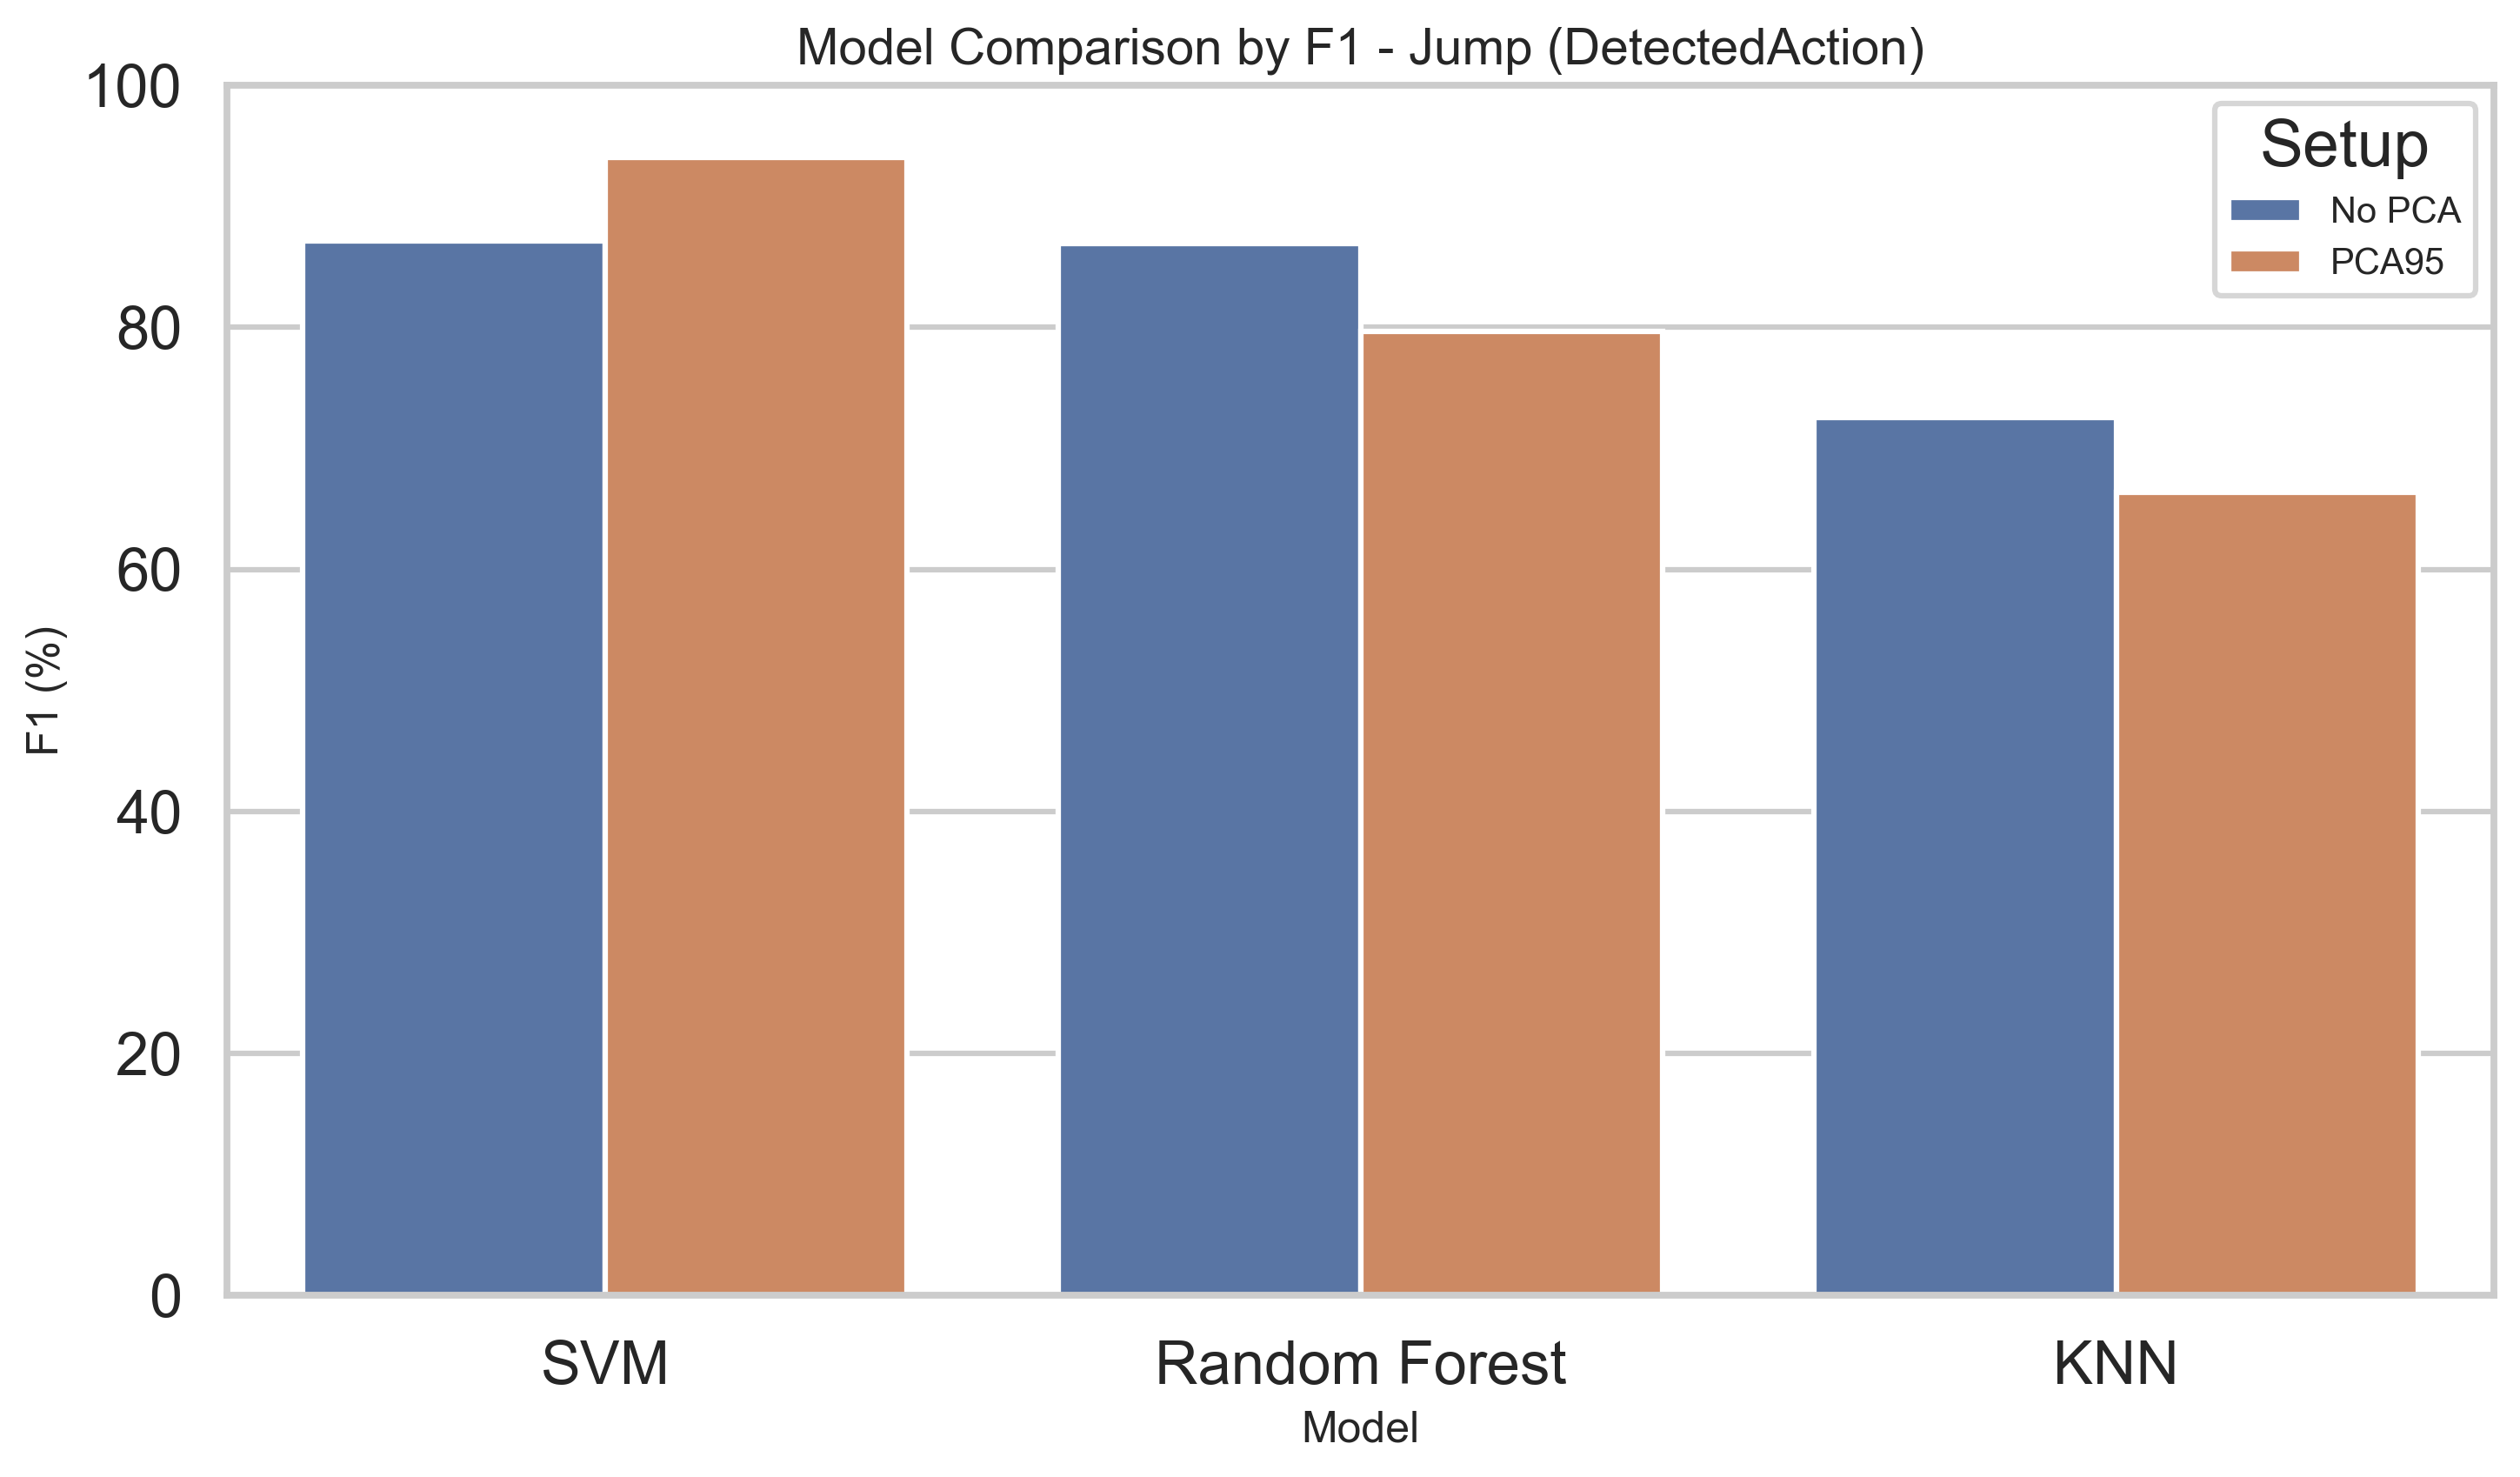
\includegraphics[width=0.85\linewidth]{Images/Generated/TaskResults/Jump/DetectedAction/model_comparison_f1.png}
    \caption{مقایسه عملکرد مدل‌ها بر اساس معیار \lr{F1} در فعالیت پریدن.}
    \label{fig:jump_detectedaction_model_comparison_f1}
\end{figure}

\noindent\textbf{توضیح شکل:} این نمودار اثر استفاده یا عدم استفاده از کاهش بعد را برای هر مدل نشان می‌دهد.
\vspace{0.8em}

\begin{figure}[H]
    \centering
    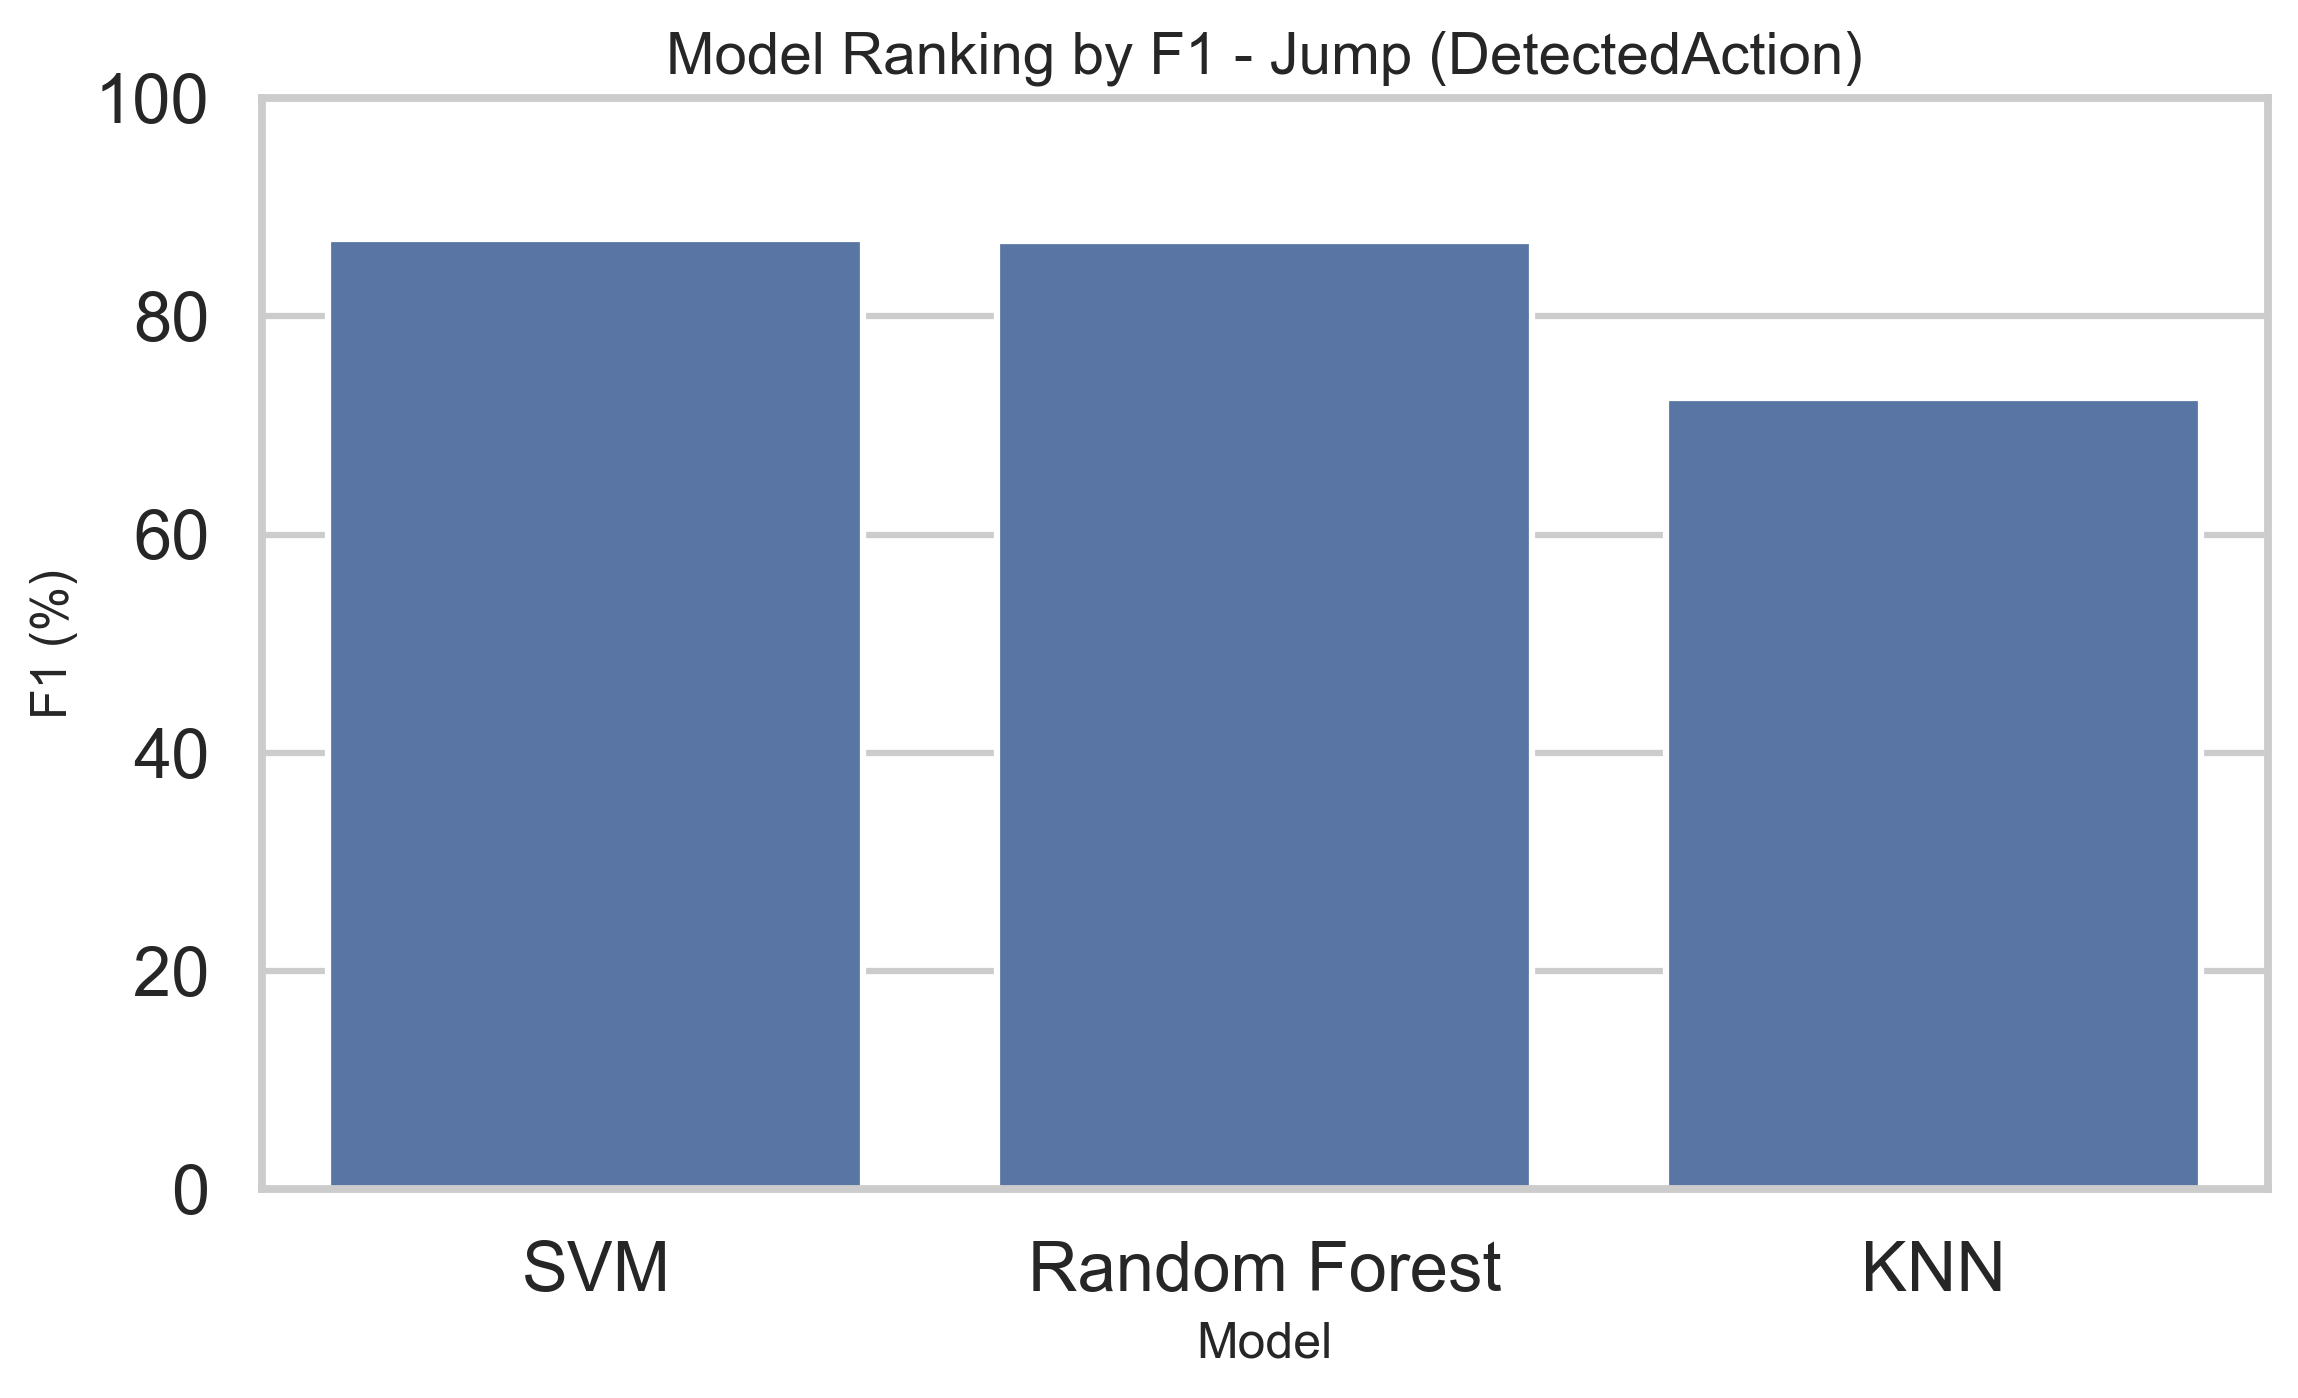
\includegraphics[width=0.85\linewidth]{Images/Generated/TaskResults/Jump/DetectedAction/model_ranking_f1.png}
    \caption{رتبه‌بندی مدل‌ها بر اساس معیار \lr{F1} در فعالیت پریدن.}
    \label{fig:jump_detectedaction_model_ranking_f1}
\end{figure}

\noindent\textbf{توضیح شکل:} این شکل جمع‌بندی سریعی از برتری نسبی مدل‌ها ارائه می‌دهد.
\vspace{0.8em}

\begin{figure}[H]
    \centering
    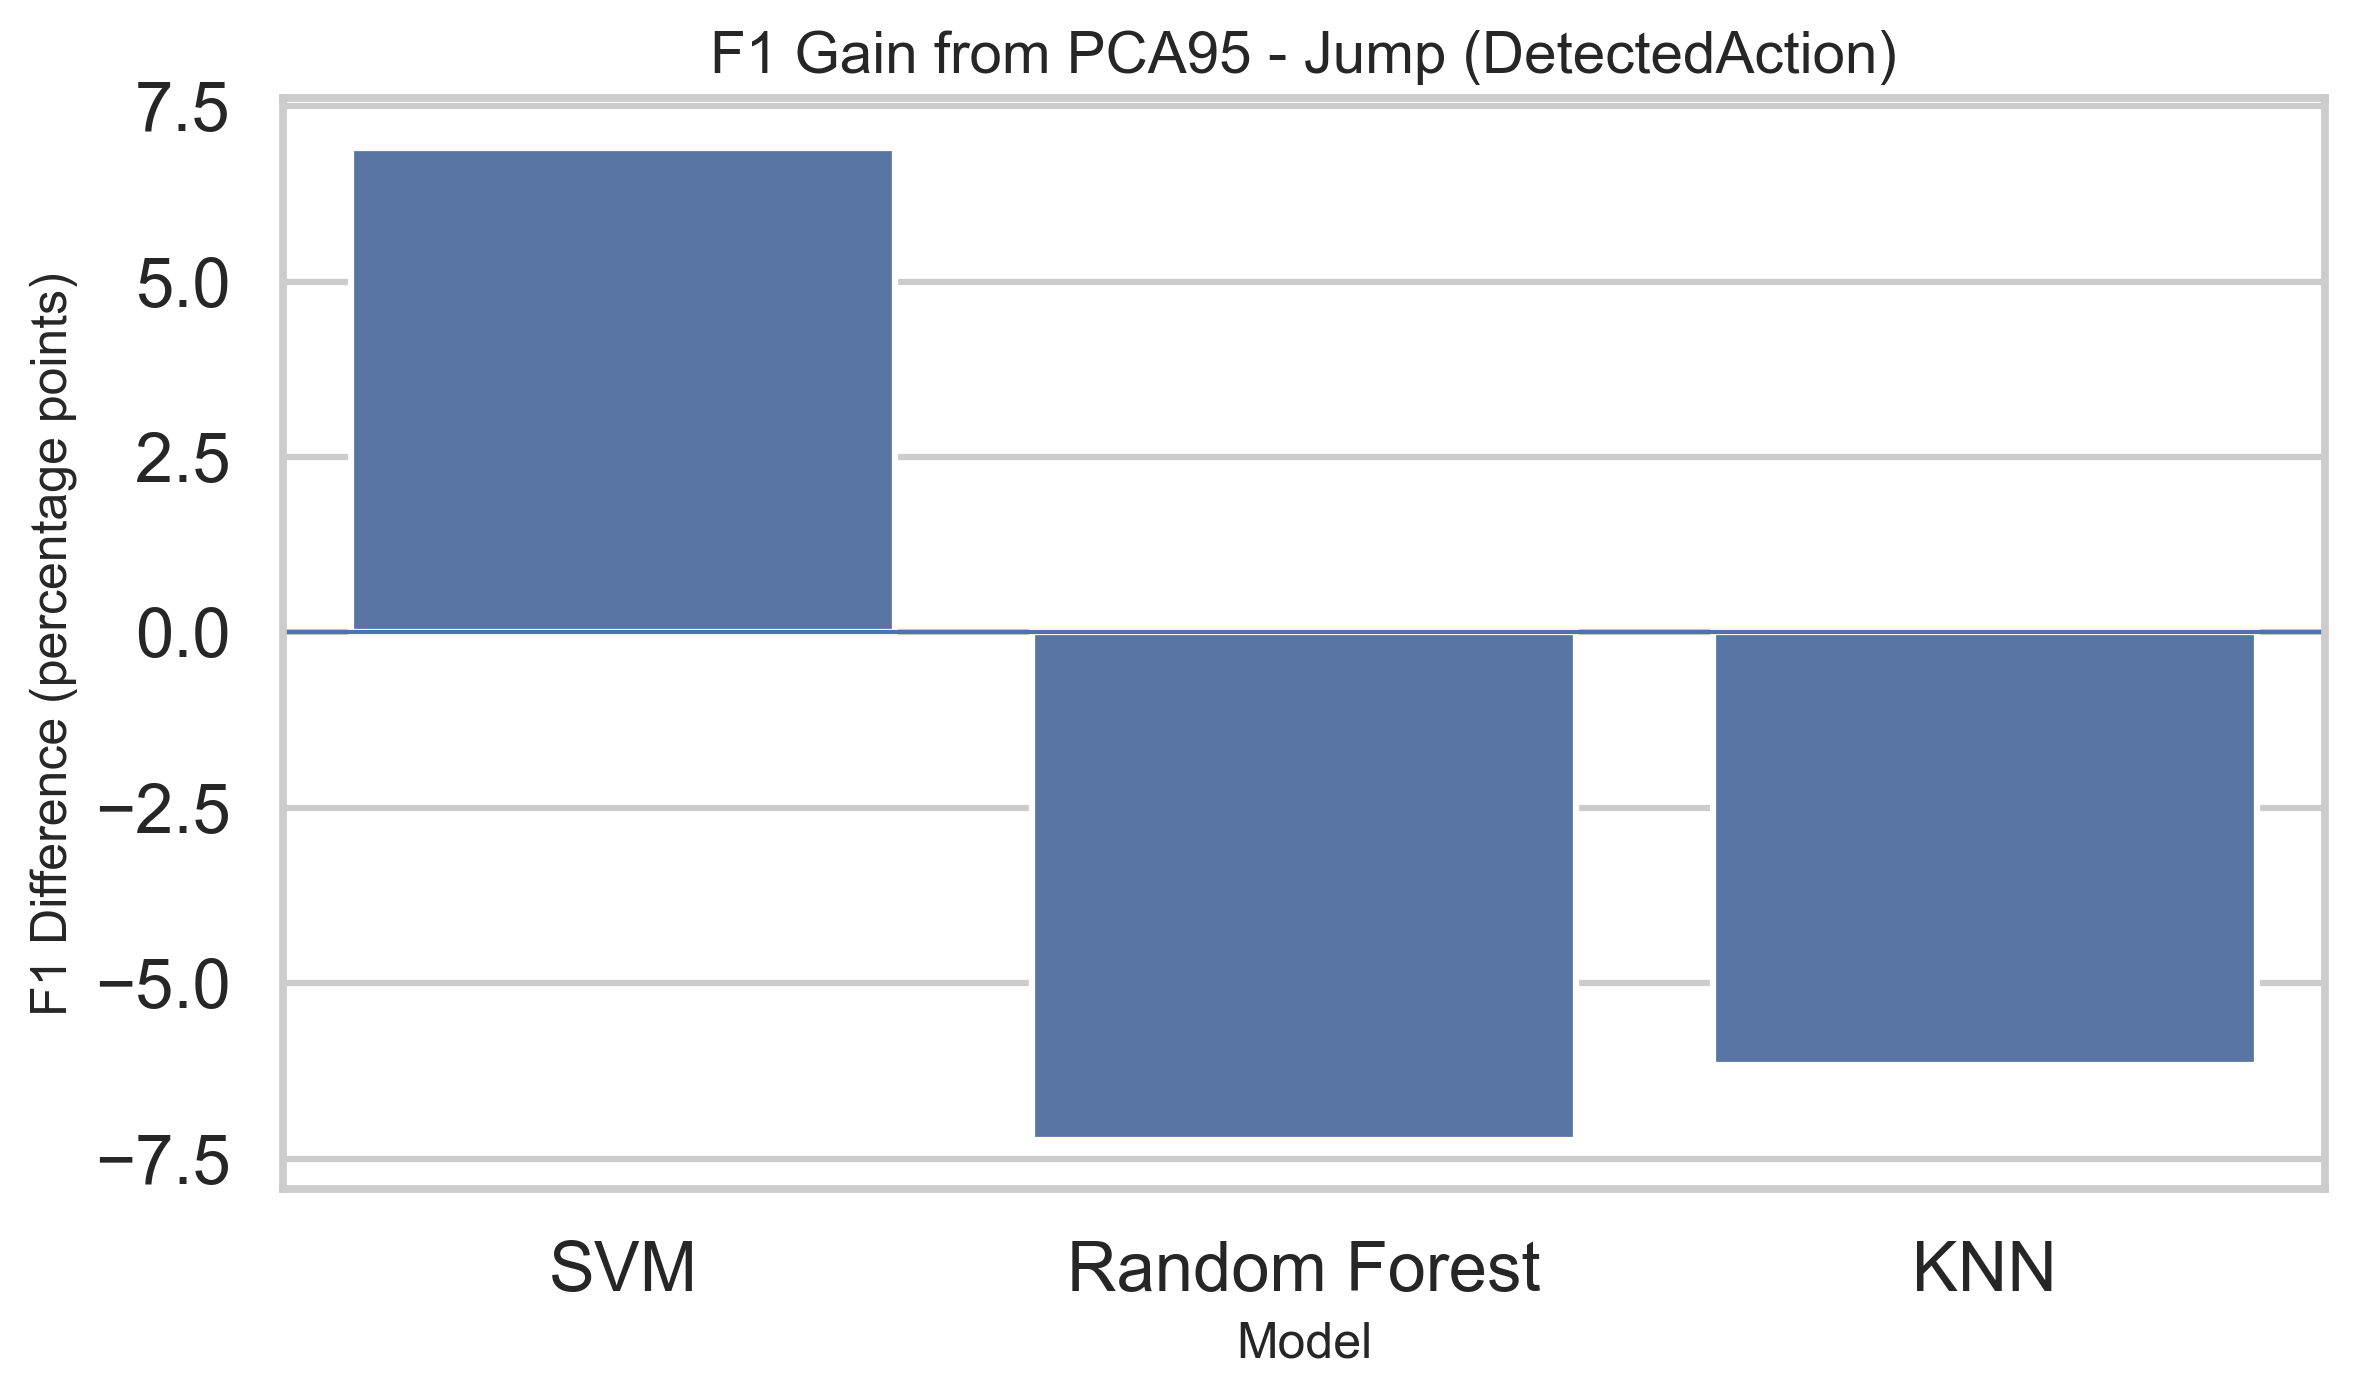
\includegraphics[width=0.85\linewidth]{Images/Generated/TaskResults/Jump/DetectedAction/f1_gain_pca_vs_no_pca.png}
    \caption{تغییر معیار \lr{F1} پس از اعمال \lr{PCA95} در فعالیت پریدن.}
    \label{fig:jump_detectedaction_f1_gain_pca}
\end{figure}

\noindent\textbf{توضیح شکل:} این شکل نشان می‌دهد کاهش بعد برای هر مدل سودمند بوده یا موجب افت عملکرد شده است.
\vspace{0.8em}

\begin{figure}[H]
    \centering
    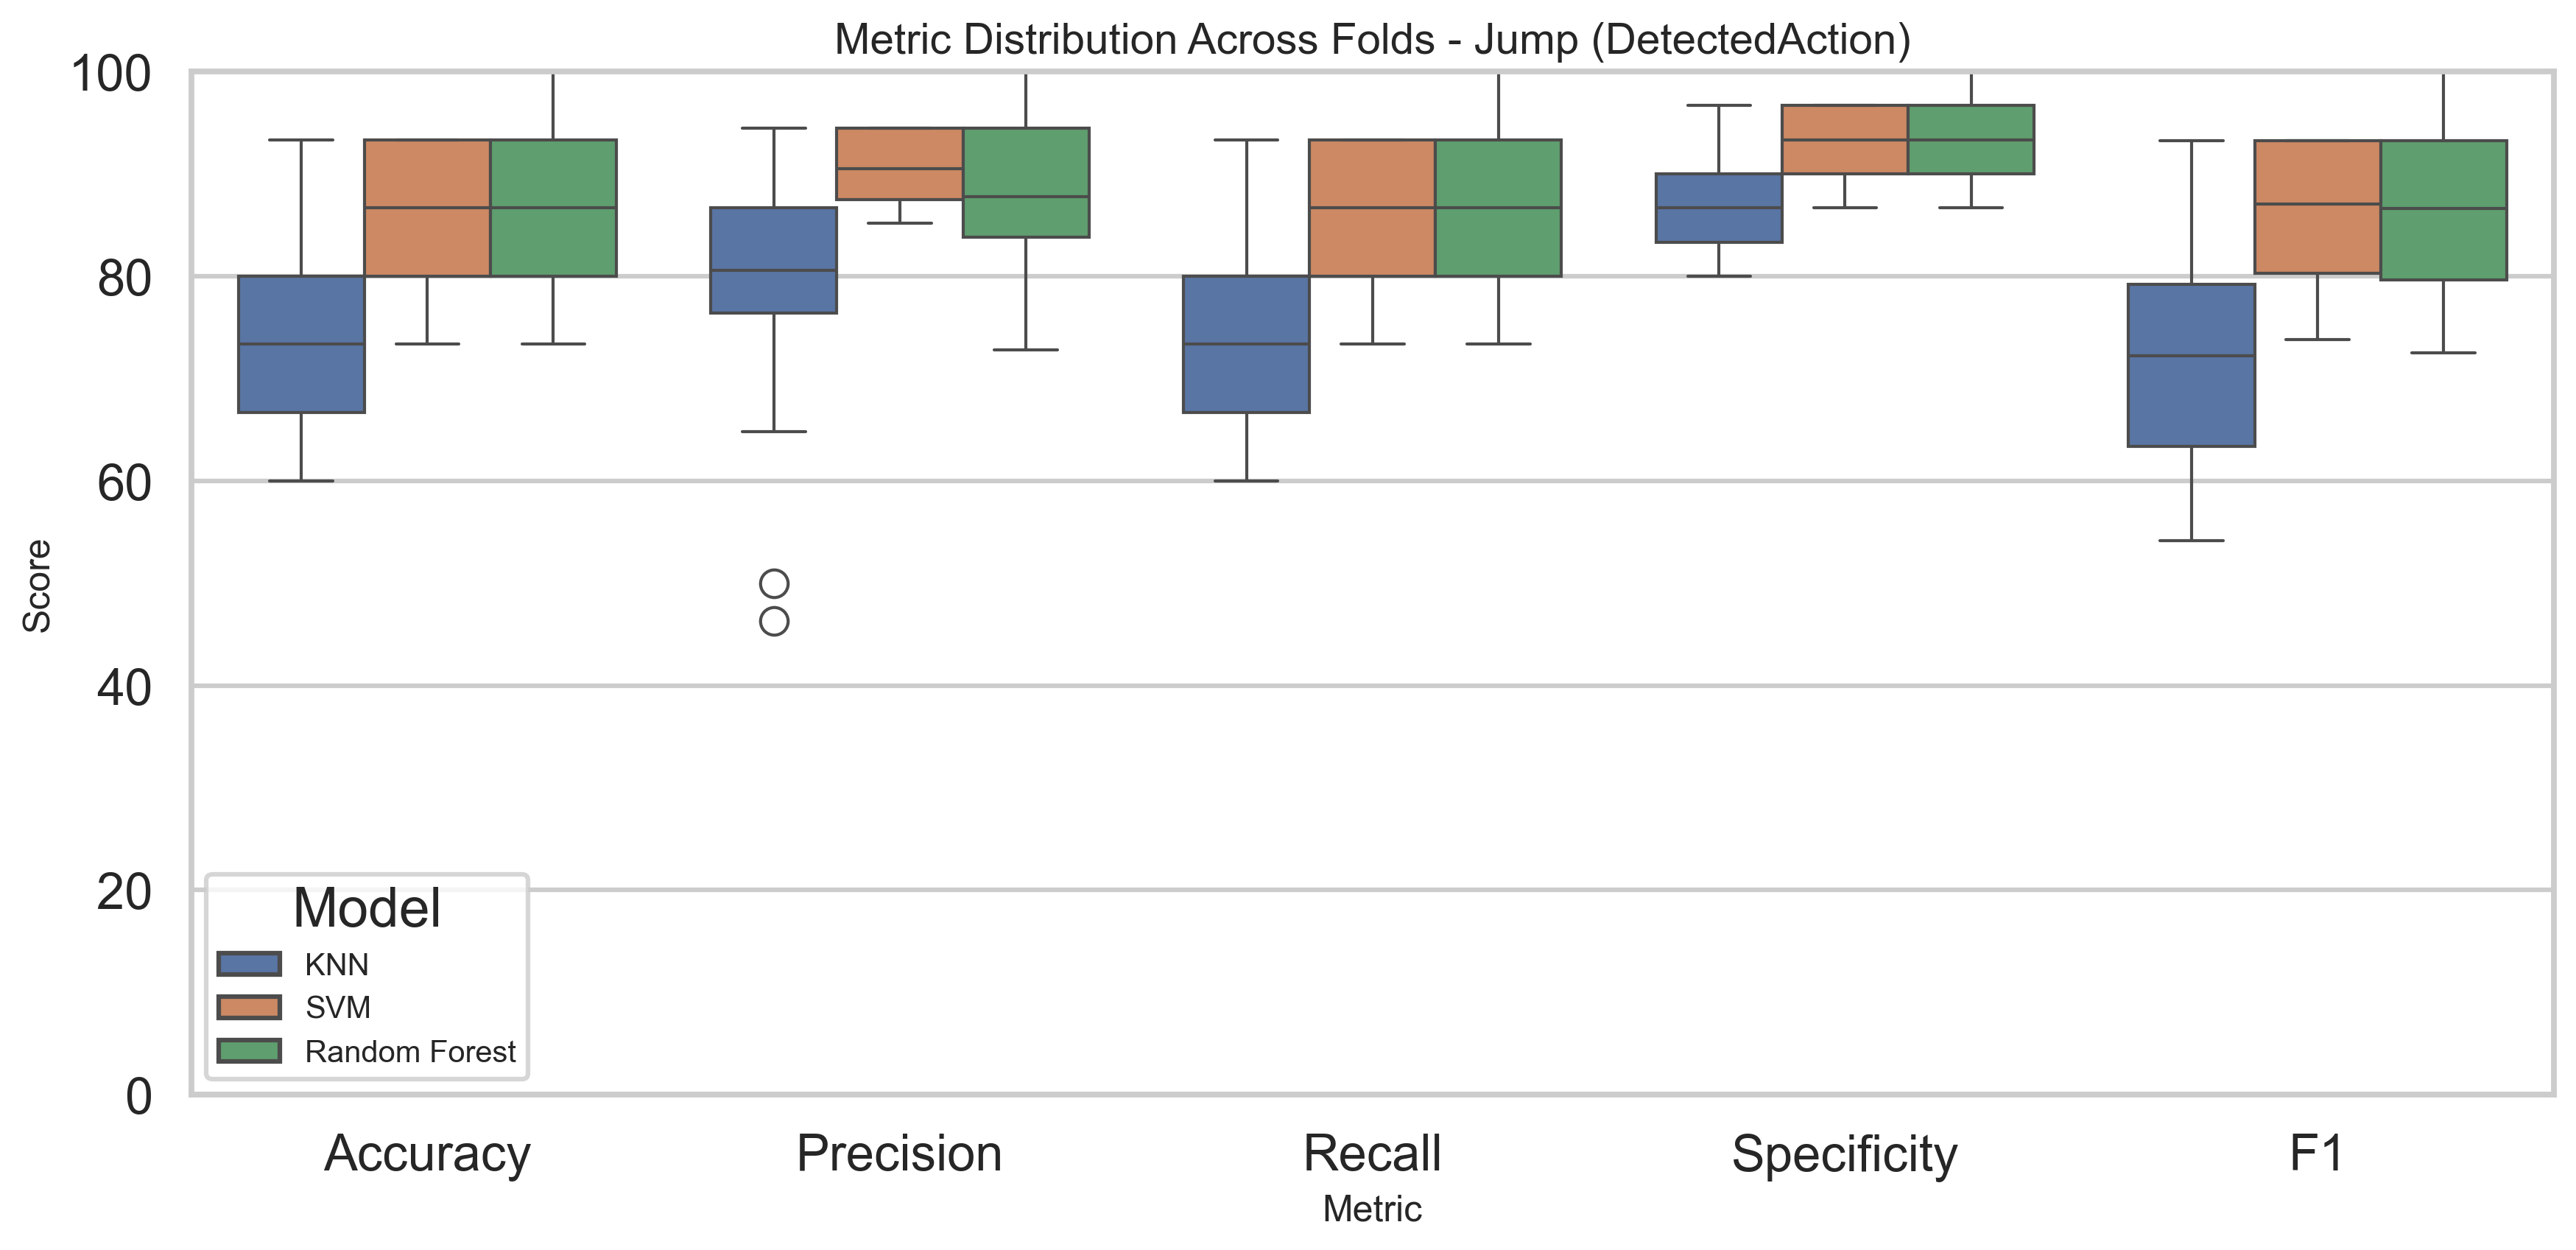
\includegraphics[width=0.85\linewidth]{Images/Generated/TaskResults/Jump/DetectedAction/metric_boxplots.png}
    \caption{پراکندگی معیارهای ارزیابی در تکرارهای اعتبارسنجی برای فعالیت پریدن.}
    \label{fig:jump_detectedaction_metric_boxplots}
\end{figure}

\noindent\textbf{توضیح شکل:} این شکل پایداری مدل‌ها را در foldهای مختلف نشان می‌دهد.
\vspace{0.8em}

\begin{figure}[H]
    \centering
    
\includegraphics[width=0.85\linewidth]{Images/Generated/TaskResults/Jump/DetectedAction/confusion_matrices_no_pca.png}
    \caption{ماتریس درهم‌ریختگی نرمال‌شده مدل‌ها در فعالیت پریدن (no_pca).}
    \label{fig:jump_detectedaction_confusion_no_pca}
\end{figure}

\noindent\textbf{توضیح شکل:} این شکل مشخص می‌کند خطاهای اصلی بین کدام کلاس‌های عملکردی رخ داده است.
\vspace{0.8em}

\begin{figure}[H]
    \centering
    
\includegraphics[width=0.85\linewidth]{Images/Generated/TaskResults/Jump/DetectedAction/per_class_recall_no_pca.png}
    \caption{مقایسه \lr{Recall} هر کلاس در فعالیت پریدن (no_pca).}
    \label{fig:jump_detectedaction_per_class_recall_no_pca}
\end{figure}

\noindent\textbf{توضیح شکل:} این نمودار حساسیت مدل‌ها نسبت به هر سطح عملکردی را نشان می‌دهد.
\vspace{0.8em}

\begin{figure}[H]
    \centering
    
\includegraphics[width=0.85\linewidth]{Images/Generated/TaskResults/Jump/DetectedAction/confusion_matrices_pca95.png}
    \caption{ماتریس درهم‌ریختگی نرمال‌شده مدل‌ها در فعالیت پریدن (pca95).}
    \label{fig:jump_detectedaction_confusion_pca95}
\end{figure}

\noindent\textbf{توضیح شکل:} این شکل مشخص می‌کند خطاهای اصلی بین کدام کلاس‌های عملکردی رخ داده است.
\vspace{0.8em}

\begin{figure}[H]
    \centering
    
\includegraphics[width=0.85\linewidth]{Images/Generated/TaskResults/Jump/DetectedAction/per_class_recall_pca95.png}
    \caption{مقایسه \lr{Recall} هر کلاس در فعالیت پریدن (pca95).}
    \label{fig:jump_detectedaction_per_class_recall_pca95}
\end{figure}

\noindent\textbf{توضیح شکل:} این نمودار حساسیت مدل‌ها نسبت به هر سطح عملکردی را نشان می‌دهد.
\vspace{0.8em}

\begin{figure}[H]
    \centering
    
\includegraphics[width=0.85\linewidth]{Images/Generated/TaskResults/Jump/DetectedAction/rf_top_feature_importance.png}
    \caption{20 ویژگی برتر بر اساس اهمیت در مدل \lr{Random Forest} برای فعالیت پریدن.}
    \label{fig:jump_detectedaction_rf_importance}
\end{figure}

\noindent\textbf{توضیح شکل:} این شکل نشان می‌دهد کدام حسگرها، محورها و شاخص‌های آماری نقش بیشتری در تصمیم‌گیری مدل داشته‌اند.
\vspace{0.8em}

\begin{figure}[H]
    \centering
    
\includegraphics[width=0.85\linewidth]{Images/Generated/TaskResults/Jump/DetectedAction/class_centroid_feature_heatmap.png}
    \caption{میانگین نرمال‌شده ویژگی‌های برتر در کلاس‌های مختلف فعالیت پریدن.}
    \label{fig:jump_detectedaction_class_centroid_heatmap}
\end{figure}

\noindent\textbf{توضیح شکل:} این نقشه حرارتی الگوی میانگین ویژگی‌ها را در هر سطح عملکردی نمایش می‌دهد.
\vspace{0.8em}

\begin{figure}[H]
    \centering
    
\includegraphics[width=0.85\linewidth]{Images/Generated/TaskResults/Jump/DetectedAction/svm_metrics_vs_pca_components.png}
    \caption{تغییر عملکرد مدل \lr{SVM} نسبت به تعداد مؤلفه‌های اصلی در فعالیت پریدن.}
    \label{fig:jump_detectedaction_svm_metrics_vs_pca_components}
\end{figure}

\noindent\textbf{توضیح شکل:} این نمودار برای انتخاب بازه مناسب تعداد مؤلفه‌های اصلی استفاده می‌شود.
\vspace{0.8em}

\begin{figure}[H]
    \centering
    
\includegraphics[width=0.85\linewidth]{Images/Generated/TaskResults/Jump/DetectedAction/models_f1_vs_pca_components.png}
    \caption{مقایسه مدل‌ها نسبت به تعداد مؤلفه‌های اصلی در فعالیت پریدن.}
    \label{fig:jump_detectedaction_models_f1_vs_pca_components}
\end{figure}

\noindent\textbf{توضیح شکل:} این نمودار نشان می‌دهد انتخاب تعداد مؤلفه‌ها و انتخاب مدل باید هم‌زمان انجام شود.
\vspace{0.8em}


\subsection*{نمودارهای فعالیت ایستادن}

\subsubsection*{داده‌های اصلی}

\begin{figure}[H]
    \centering
    
\includegraphics[width=0.85\linewidth]{Images/Generated/TaskResults/Stand/Normal/signal_sample.png}
    \caption{نمونه سیگنال‌های ثبت‌شده در فعالیت ایستادن (داده‌های اصلی).}
    \label{fig:stand_normal_signal_sample}
\end{figure}

\noindent\textbf{توضیح شکل:} این شکل نمایی از ماهیت زمانی سیگنال‌های حسگرها را برای فعالیت مورد نظر نشان می‌دهد.
\vspace{0.8em}

\begin{figure}[H]
    \centering
    
\includegraphics[width=0.85\linewidth]{Images/Generated/TaskResults/Stand/Normal/class_distribution.png}
    \caption{توزیع تعداد نمونه‌ها در سطوح عملکردی فعالیت ایستادن.}
    \label{fig:stand_normal_class_distribution}
\end{figure}

\noindent\textbf{توضیح شکل:} این نمودار برای بررسی تعادل داده‌ها بین کلاس‌های صفر، یک و دو استفاده می‌شود.
\vspace{0.8em}

\begin{figure}[H]
    \centering
    
\includegraphics[width=0.85\linewidth]{Images/Generated/TaskResults/Stand/Normal/feature_correlation_heatmap.png}
    \caption{نقشه همبستگی 20 ویژگی با بیشترین واریانس در فعالیت ایستادن.}
    \label{fig:stand_normal_feature_correlation}
\end{figure}

\noindent\textbf{توضیح شکل:} این نمودار وجود اطلاعات تکراری در فضای ویژگی را نشان می‌دهد و استفاده از کاهش بعد را توجیه می‌کند.
\vspace{0.8em}

\begin{figure}[H]
    \centering
    
\includegraphics[width=0.85\linewidth]{Images/Generated/TaskResults/Stand/Normal/pca_variance_curve.png}
    \caption{درصد واریانس توضیح‌داده‌شده و واریانس تجمعی مؤلفه‌های اصلی در فعالیت ایستادن.}
    \label{fig:stand_normal_pca_variance}
\end{figure}

\noindent\textbf{توضیح شکل:} این شکل مبنای انتخاب آستانه ۹۵ درصد و تعیین تعداد مؤلفه‌های نگه‌داشته‌شده را نشان می‌دهد.
\vspace{0.8em}

\begin{figure}[H]
    \centering
    
\includegraphics[width=0.85\linewidth]{Images/Generated/TaskResults/Stand/Normal/pca_scatter_pc1_pc2.png}
    \caption{پراکندگی نمونه‌های فعالیت ایستادن در فضای دو مؤلفه اصلی اول.}
    \label{fig:stand_normal_pca_scatter}
\end{figure}

\noindent\textbf{توضیح شکل:} این شکل یک تصویر اولیه از جدایی یا هم‌پوشانی کلاس‌ها در فضای کاهش‌یافته ارائه می‌دهد.
\vspace{0.8em}

\begin{figure}[H]
    \centering
    
\includegraphics[width=0.85\linewidth]{Images/Generated/TaskResults/Stand/Normal/model_comparison_f1.png}
    \caption{مقایسه عملکرد مدل‌ها بر اساس معیار \lr{F1} در فعالیت ایستادن.}
    \label{fig:stand_normal_model_comparison_f1}
\end{figure}

\noindent\textbf{توضیح شکل:} این نمودار اثر استفاده یا عدم استفاده از کاهش بعد را برای هر مدل نشان می‌دهد.
\vspace{0.8em}

\begin{figure}[H]
    \centering
    
\includegraphics[width=0.85\linewidth]{Images/Generated/TaskResults/Stand/Normal/model_ranking_f1.png}
    \caption{رتبه‌بندی مدل‌ها بر اساس معیار \lr{F1} در فعالیت ایستادن.}
    \label{fig:stand_normal_model_ranking_f1}
\end{figure}

\noindent\textbf{توضیح شکل:} این شکل جمع‌بندی سریعی از برتری نسبی مدل‌ها ارائه می‌دهد.
\vspace{0.8em}

\begin{figure}[H]
    \centering
    
\includegraphics[width=0.85\linewidth]{Images/Generated/TaskResults/Stand/Normal/f1_gain_pca_vs_no_pca.png}
    \caption{تغییر معیار \lr{F1} پس از اعمال \lr{PCA95} در فعالیت ایستادن.}
    \label{fig:stand_normal_f1_gain_pca}
\end{figure}

\noindent\textbf{توضیح شکل:} این شکل نشان می‌دهد کاهش بعد برای هر مدل سودمند بوده یا موجب افت عملکرد شده است.
\vspace{0.8em}

\begin{figure}[H]
    \centering
    
\includegraphics[width=0.85\linewidth]{Images/Generated/TaskResults/Stand/Normal/metric_boxplots.png}
    \caption{پراکندگی معیارهای ارزیابی در تکرارهای اعتبارسنجی برای فعالیت ایستادن.}
    \label{fig:stand_normal_metric_boxplots}
\end{figure}

\noindent\textbf{توضیح شکل:} این شکل پایداری مدل‌ها را در foldهای مختلف نشان می‌دهد.
\vspace{0.8em}

\begin{figure}[H]
    \centering
    
\includegraphics[width=0.85\linewidth]{Images/Generated/TaskResults/Stand/Normal/confusion_matrices_no_pca.png}
    \caption{ماتریس درهم‌ریختگی نرمال‌شده مدل‌ها در فعالیت ایستادن (no_pca).}
    \label{fig:stand_normal_confusion_no_pca}
\end{figure}

\noindent\textbf{توضیح شکل:} این شکل مشخص می‌کند خطاهای اصلی بین کدام کلاس‌های عملکردی رخ داده است.
\vspace{0.8em}

\begin{figure}[H]
    \centering
    
\includegraphics[width=0.85\linewidth]{Images/Generated/TaskResults/Stand/Normal/per_class_recall_no_pca.png}
    \caption{مقایسه \lr{Recall} هر کلاس در فعالیت ایستادن (no_pca).}
    \label{fig:stand_normal_per_class_recall_no_pca}
\end{figure}

\noindent\textbf{توضیح شکل:} این نمودار حساسیت مدل‌ها نسبت به هر سطح عملکردی را نشان می‌دهد.
\vspace{0.8em}

\begin{figure}[H]
    \centering
    
\includegraphics[width=0.85\linewidth]{Images/Generated/TaskResults/Stand/Normal/confusion_matrices_pca95.png}
    \caption{ماتریس درهم‌ریختگی نرمال‌شده مدل‌ها در فعالیت ایستادن (pca95).}
    \label{fig:stand_normal_confusion_pca95}
\end{figure}

\noindent\textbf{توضیح شکل:} این شکل مشخص می‌کند خطاهای اصلی بین کدام کلاس‌های عملکردی رخ داده است.
\vspace{0.8em}

\begin{figure}[H]
    \centering
    
\includegraphics[width=0.85\linewidth]{Images/Generated/TaskResults/Stand/Normal/per_class_recall_pca95.png}
    \caption{مقایسه \lr{Recall} هر کلاس در فعالیت ایستادن (pca95).}
    \label{fig:stand_normal_per_class_recall_pca95}
\end{figure}

\noindent\textbf{توضیح شکل:} این نمودار حساسیت مدل‌ها نسبت به هر سطح عملکردی را نشان می‌دهد.
\vspace{0.8em}

\begin{figure}[H]
    \centering
    
\includegraphics[width=0.85\linewidth]{Images/Generated/TaskResults/Stand/Normal/rf_top_feature_importance.png}
    \caption{20 ویژگی برتر بر اساس اهمیت در مدل \lr{Random Forest} برای فعالیت ایستادن.}
    \label{fig:stand_normal_rf_importance}
\end{figure}

\noindent\textbf{توضیح شکل:} این شکل نشان می‌دهد کدام حسگرها، محورها و شاخص‌های آماری نقش بیشتری در تصمیم‌گیری مدل داشته‌اند.
\vspace{0.8em}

\begin{figure}[H]
    \centering
    
\includegraphics[width=0.85\linewidth]{Images/Generated/TaskResults/Stand/Normal/class_centroid_feature_heatmap.png}
    \caption{میانگین نرمال‌شده ویژگی‌های برتر در کلاس‌های مختلف فعالیت ایستادن.}
    \label{fig:stand_normal_class_centroid_heatmap}
\end{figure}

\noindent\textbf{توضیح شکل:} این نقشه حرارتی الگوی میانگین ویژگی‌ها را در هر سطح عملکردی نمایش می‌دهد.
\vspace{0.8em}

\begin{figure}[H]
    \centering
    
\includegraphics[width=0.85\linewidth]{Images/Generated/TaskResults/Stand/Normal/svm_metrics_vs_pca_components.png}
    \caption{تغییر عملکرد مدل \lr{SVM} نسبت به تعداد مؤلفه‌های اصلی در فعالیت ایستادن.}
    \label{fig:stand_normal_svm_metrics_vs_pca_components}
\end{figure}

\noindent\textbf{توضیح شکل:} این نمودار برای انتخاب بازه مناسب تعداد مؤلفه‌های اصلی استفاده می‌شود.
\vspace{0.8em}

\begin{figure}[H]
    \centering
    
\includegraphics[width=0.85\linewidth]{Images/Generated/TaskResults/Stand/Normal/models_f1_vs_pca_components.png}
    \caption{مقایسه مدل‌ها نسبت به تعداد مؤلفه‌های اصلی در فعالیت ایستادن.}
    \label{fig:stand_normal_models_f1_vs_pca_components}
\end{figure}

\noindent\textbf{توضیح شکل:} این نمودار نشان می‌دهد انتخاب تعداد مؤلفه‌ها و انتخاب مدل باید هم‌زمان انجام شود.
\vspace{0.8em}

\subsection*{نمودارهای فعالیت بلند شدن از صندلی}

\subsubsection*{داده‌های اصلی}

\begin{figure}[H]
    \centering
    
\includegraphics[width=0.85\linewidth]{Images/Generated/TaskResults/Sit_To_Stand/Normal/signal_sample.png}
    \caption{نمونه سیگنال‌های ثبت‌شده در فعالیت بلند شدن از صندلی (داده‌های اصلی).}
    \label{fig:sit_to_stand_normal_signal_sample}
\end{figure}

\noindent\textbf{توضیح شکل:} این شکل نمایی از ماهیت زمانی سیگنال‌های حسگرها را برای فعالیت مورد نظر نشان می‌دهد.
\vspace{0.8em}

\begin{figure}[H]
    \centering
    
\includegraphics[width=0.85\linewidth]{Images/Generated/TaskResults/Sit_To_Stand/Normal/class_distribution.png}
    \caption{توزیع تعداد نمونه‌ها در سطوح عملکردی فعالیت بلند شدن از صندلی.}
    \label{fig:sit_to_stand_normal_class_distribution}
\end{figure}

\noindent\textbf{توضیح شکل:} این نمودار برای بررسی تعادل داده‌ها بین کلاس‌های صفر، یک و دو استفاده می‌شود.
\vspace{0.8em}

\begin{figure}[H]
    \centering
    
\includegraphics[width=0.85\linewidth]{Images/Generated/TaskResults/Sit_To_Stand/Normal/feature_correlation_heatmap.png}
    \caption{نقشه همبستگی 20 ویژگی با بیشترین واریانس در فعالیت بلند شدن از صندلی.}
    \label{fig:sit_to_stand_normal_feature_correlation}
\end{figure}

\noindent\textbf{توضیح شکل:} این نمودار وجود اطلاعات تکراری در فضای ویژگی را نشان می‌دهد و استفاده از کاهش بعد را توجیه می‌کند.
\vspace{0.8em}

\begin{figure}[H]
    \centering
    
\includegraphics[width=0.85\linewidth]{Images/Generated/TaskResults/Sit_To_Stand/Normal/pca_variance_curve.png}
    \caption{درصد واریانس توضیح‌داده‌شده و واریانس تجمعی مؤلفه‌های اصلی در فعالیت بلند شدن از صندلی.}
    \label{fig:sit_to_stand_normal_pca_variance}
\end{figure}

\noindent\textbf{توضیح شکل:} این شکل مبنای انتخاب آستانه ۹۵ درصد و تعیین تعداد مؤلفه‌های نگه‌داشته‌شده را نشان می‌دهد.
\vspace{0.8em}

\begin{figure}[H]
    \centering
    
\includegraphics[width=0.85\linewidth]{Images/Generated/TaskResults/Sit_To_Stand/Normal/pca_scatter_pc1_pc2.png}
    \caption{پراکندگی نمونه‌های فعالیت بلند شدن از صندلی در فضای دو مؤلفه اصلی اول.}
    \label{fig:sit_to_stand_normal_pca_scatter}
\end{figure}

\noindent\textbf{توضیح شکل:} این شکل یک تصویر اولیه از جدایی یا هم‌پوشانی کلاس‌ها در فضای کاهش‌یافته ارائه می‌دهد.
\vspace{0.8em}

\begin{figure}[H]
    \centering
    
\includegraphics[width=0.85\linewidth]{Images/Generated/TaskResults/Sit_To_Stand/Normal/model_comparison_f1.png}
    \caption{مقایسه عملکرد مدل‌ها بر اساس معیار \lr{F1} در فعالیت بلند شدن از صندلی.}
    \label{fig:sit_to_stand_normal_model_comparison_f1}
\end{figure}

\noindent\textbf{توضیح شکل:} این نمودار اثر استفاده یا عدم استفاده از کاهش بعد را برای هر مدل نشان می‌دهد.
\vspace{0.8em}

\begin{figure}[H]
    \centering
    
\includegraphics[width=0.85\linewidth]{Images/Generated/TaskResults/Sit_To_Stand/Normal/model_ranking_f1.png}
    \caption{رتبه‌بندی مدل‌ها بر اساس معیار \lr{F1} در فعالیت بلند شدن از صندلی.}
    \label{fig:sit_to_stand_normal_model_ranking_f1}
\end{figure}

\noindent\textbf{توضیح شکل:} این شکل جمع‌بندی سریعی از برتری نسبی مدل‌ها ارائه می‌دهد.
\vspace{0.8em}

\begin{figure}[H]
    \centering
    
\includegraphics[width=0.85\linewidth]{Images/Generated/TaskResults/Sit_To_Stand/Normal/f1_gain_pca_vs_no_pca.png}
    \caption{تغییر معیار \lr{F1} پس از اعمال \lr{PCA95} در فعالیت بلند شدن از صندلی.}
    \label{fig:sit_to_stand_normal_f1_gain_pca}
\end{figure}

\noindent\textbf{توضیح شکل:} این شکل نشان می‌دهد کاهش بعد برای هر مدل سودمند بوده یا موجب افت عملکرد شده است.
\vspace{0.8em}

\begin{figure}[H]
    \centering
    
\includegraphics[width=0.85\linewidth]{Images/Generated/TaskResults/Sit_To_Stand/Normal/metric_boxplots.png}
    \caption{پراکندگی معیارهای ارزیابی در تکرارهای اعتبارسنجی برای فعالیت بلند شدن از صندلی.}
    \label{fig:sit_to_stand_normal_metric_boxplots}
\end{figure}

\noindent\textbf{توضیح شکل:} این شکل پایداری مدل‌ها را در foldهای مختلف نشان می‌دهد.
\vspace{0.8em}

\begin{figure}[H]
    \centering
    
\includegraphics[width=0.85\linewidth]{Images/Generated/TaskResults/Sit_To_Stand/Normal/confusion_matrices_no_pca.png}
    \caption{ماتریس درهم‌ریختگی نرمال‌شده مدل‌ها در فعالیت بلند شدن از صندلی (no_pca).}
    \label{fig:sit_to_stand_normal_confusion_no_pca}
\end{figure}

\noindent\textbf{توضیح شکل:} این شکل مشخص می‌کند خطاهای اصلی بین کدام کلاس‌های عملکردی رخ داده است.
\vspace{0.8em}

\begin{figure}[H]
    \centering
    
\includegraphics[width=0.85\linewidth]{Images/Generated/TaskResults/Sit_To_Stand/Normal/per_class_recall_no_pca.png}
    \caption{مقایسه \lr{Recall} هر کلاس در فعالیت بلند شدن از صندلی (no_pca).}
    \label{fig:sit_to_stand_normal_per_class_recall_no_pca}
\end{figure}

\noindent\textbf{توضیح شکل:} این نمودار حساسیت مدل‌ها نسبت به هر سطح عملکردی را نشان می‌دهد.
\vspace{0.8em}

\begin{figure}[H]
    \centering
    
\includegraphics[width=0.85\linewidth]{Images/Generated/TaskResults/Sit_To_Stand/Normal/confusion_matrices_pca95.png}
    \caption{ماتریس درهم‌ریختگی نرمال‌شده مدل‌ها در فعالیت بلند شدن از صندلی (pca95).}
    \label{fig:sit_to_stand_normal_confusion_pca95}
\end{figure}

\noindent\textbf{توضیح شکل:} این شکل مشخص می‌کند خطاهای اصلی بین کدام کلاس‌های عملکردی رخ داده است.
\vspace{0.8em}

\begin{figure}[H]
    \centering
    
\includegraphics[width=0.85\linewidth]{Images/Generated/TaskResults/Sit_To_Stand/Normal/per_class_recall_pca95.png}
    \caption{مقایسه \lr{Recall} هر کلاس در فعالیت بلند شدن از صندلی (pca95).}
    \label{fig:sit_to_stand_normal_per_class_recall_pca95}
\end{figure}

\noindent\textbf{توضیح شکل:} این نمودار حساسیت مدل‌ها نسبت به هر سطح عملکردی را نشان می‌دهد.
\vspace{0.8em}

\begin{figure}[H]
    \centering
    
\includegraphics[width=0.85\linewidth]{Images/Generated/TaskResults/Sit_To_Stand/Normal/rf_top_feature_importance.png}
    \caption{20 ویژگی برتر بر اساس اهمیت در مدل \lr{Random Forest} برای فعالیت بلند شدن از صندلی.}
    \label{fig:sit_to_stand_normal_rf_importance}
\end{figure}

\noindent\textbf{توضیح شکل:} این شکل نشان می‌دهد کدام حسگرها، محورها و شاخص‌های آماری نقش بیشتری در تصمیم‌گیری مدل داشته‌اند.
\vspace{0.8em}

\begin{figure}[H]
    \centering
    
\includegraphics[width=0.85\linewidth]{Images/Generated/TaskResults/Sit_To_Stand/Normal/class_centroid_feature_heatmap.png}
    \caption{میانگین نرمال‌شده ویژگی‌های برتر در کلاس‌های مختلف فعالیت بلند شدن از صندلی.}
    \label{fig:sit_to_stand_normal_class_centroid_heatmap}
\end{figure}

\noindent\textbf{توضیح شکل:} این نقشه حرارتی الگوی میانگین ویژگی‌ها را در هر سطح عملکردی نمایش می‌دهد.
\vspace{0.8em}

\begin{figure}[H]
    \centering
    
\includegraphics[width=0.85\linewidth]{Images/Generated/TaskResults/Sit_To_Stand/Normal/svm_metrics_vs_pca_components.png}
    \caption{تغییر عملکرد مدل \lr{SVM} نسبت به تعداد مؤلفه‌های اصلی در فعالیت بلند شدن از صندلی.}
    \label{fig:sit_to_stand_normal_svm_metrics_vs_pca_components}
\end{figure}

\noindent\textbf{توضیح شکل:} این نمودار برای انتخاب بازه مناسب تعداد مؤلفه‌های اصلی استفاده می‌شود.
\vspace{0.8em}

\begin{figure}[H]
    \centering
    
\includegraphics[width=0.85\linewidth]{Images/Generated/TaskResults/Sit_To_Stand/Normal/models_f1_vs_pca_components.png}
    \caption{مقایسه مدل‌ها نسبت به تعداد مؤلفه‌های اصلی در فعالیت بلند شدن از صندلی.}
    \label{fig:sit_to_stand_normal_models_f1_vs_pca_components}
\end{figure}

\noindent\textbf{توضیح شکل:} این نمودار نشان می‌دهد انتخاب تعداد مؤلفه‌ها و انتخاب مدل باید هم‌زمان انجام شود.
\vspace{0.8em}

\subsubsection*{داده‌های جداسازی‌شده با تشخیص فعالیت}

\begin{figure}[H]
    \centering
    
\includegraphics[width=0.85\linewidth]{Images/Generated/TaskResults/Sit_To_Stand/DetectedAction/signal_sample.png}
    \caption{نمونه سیگنال‌های ثبت‌شده در فعالیت بلند شدن از صندلی (داده‌های جداسازی‌شده با تشخیص فعالیت).}
    \label{fig:sit_to_stand_detectedaction_signal_sample}
\end{figure}

\noindent\textbf{توضیح شکل:} این شکل نمایی از ماهیت زمانی سیگنال‌های حسگرها را برای فعالیت مورد نظر نشان می‌دهد.
\vspace{0.8em}

\begin{figure}[H]
    \centering
    
\includegraphics[width=0.85\linewidth]{Images/Generated/TaskResults/Sit_To_Stand/DetectedAction/class_distribution.png}
    \caption{توزیع تعداد نمونه‌ها در سطوح عملکردی فعالیت بلند شدن از صندلی.}
    \label{fig:sit_to_stand_detectedaction_class_distribution}
\end{figure}

\noindent\textbf{توضیح شکل:} این نمودار برای بررسی تعادل داده‌ها بین کلاس‌های صفر، یک و دو استفاده می‌شود.
\vspace{0.8em}

\begin{figure}[H]
    \centering
    
\includegraphics[width=0.85\linewidth]{Images/Generated/TaskResults/Sit_To_Stand/DetectedAction/feature_correlation_heatmap.png}
    \caption{نقشه همبستگی 20 ویژگی با بیشترین واریانس در فعالیت بلند شدن از صندلی.}
    \label{fig:sit_to_stand_detectedaction_feature_correlation}
\end{figure}

\noindent\textbf{توضیح شکل:} این نمودار وجود اطلاعات تکراری در فضای ویژگی را نشان می‌دهد و استفاده از کاهش بعد را توجیه می‌کند.
\vspace{0.8em}

\begin{figure}[H]
    \centering
    
\includegraphics[width=0.85\linewidth]{Images/Generated/TaskResults/Sit_To_Stand/DetectedAction/pca_variance_curve.png}
    \caption{درصد واریانس توضیح‌داده‌شده و واریانس تجمعی مؤلفه‌های اصلی در فعالیت بلند شدن از صندلی.}
    \label{fig:sit_to_stand_detectedaction_pca_variance}
\end{figure}

\noindent\textbf{توضیح شکل:} این شکل مبنای انتخاب آستانه ۹۵ درصد و تعیین تعداد مؤلفه‌های نگه‌داشته‌شده را نشان می‌دهد.
\vspace{0.8em}

\begin{figure}[H]
    \centering
    
\includegraphics[width=0.85\linewidth]{Images/Generated/TaskResults/Sit_To_Stand/DetectedAction/pca_scatter_pc1_pc2.png}
    \caption{پراکندگی نمونه‌های فعالیت بلند شدن از صندلی در فضای دو مؤلفه اصلی اول.}
    \label{fig:sit_to_stand_detectedaction_pca_scatter}
\end{figure}

\noindent\textbf{توضیح شکل:} این شکل یک تصویر اولیه از جدایی یا هم‌پوشانی کلاس‌ها در فضای کاهش‌یافته ارائه می‌دهد.
\vspace{0.8em}

\begin{figure}[H]
    \centering
    
\includegraphics[width=0.85\linewidth]{Images/Generated/TaskResults/Sit_To_Stand/DetectedAction/model_comparison_f1.png}
    \caption{مقایسه عملکرد مدل‌ها بر اساس معیار \lr{F1} در فعالیت بلند شدن از صندلی.}
    \label{fig:sit_to_stand_detectedaction_model_comparison_f1}
\end{figure}

\noindent\textbf{توضیح شکل:} این نمودار اثر استفاده یا عدم استفاده از کاهش بعد را برای هر مدل نشان می‌دهد.
\vspace{0.8em}

\begin{figure}[H]
    \centering
    
\includegraphics[width=0.85\linewidth]{Images/Generated/TaskResults/Sit_To_Stand/DetectedAction/model_ranking_f1.png}
    \caption{رتبه‌بندی مدل‌ها بر اساس معیار \lr{F1} در فعالیت بلند شدن از صندلی.}
    \label{fig:sit_to_stand_detectedaction_model_ranking_f1}
\end{figure}

\noindent\textbf{توضیح شکل:} این شکل جمع‌بندی سریعی از برتری نسبی مدل‌ها ارائه می‌دهد.
\vspace{0.8em}

\begin{figure}[H]
    \centering
    
\includegraphics[width=0.85\linewidth]{Images/Generated/TaskResults/Sit_To_Stand/DetectedAction/f1_gain_pca_vs_no_pca.png}
    \caption{تغییر معیار \lr{F1} پس از اعمال \lr{PCA95} در فعالیت بلند شدن از صندلی.}
    \label{fig:sit_to_stand_detectedaction_f1_gain_pca}
\end{figure}

\noindent\textbf{توضیح شکل:} این شکل نشان می‌دهد کاهش بعد برای هر مدل سودمند بوده یا موجب افت عملکرد شده است.
\vspace{0.8em}

\begin{figure}[H]
    \centering
    
\includegraphics[width=0.85\linewidth]{Images/Generated/TaskResults/Sit_To_Stand/DetectedAction/metric_boxplots.png}
    \caption{پراکندگی معیارهای ارزیابی در تکرارهای اعتبارسنجی برای فعالیت بلند شدن از صندلی.}
    \label{fig:sit_to_stand_detectedaction_metric_boxplots}
\end{figure}

\noindent\textbf{توضیح شکل:} این شکل پایداری مدل‌ها را در foldهای مختلف نشان می‌دهد.
\vspace{0.8em}

\begin{figure}[H]
    \centering
    
\includegraphics[width=0.85\linewidth]{Images/Generated/TaskResults/Sit_To_Stand/DetectedAction/confusion_matrices_no_pca.png}
    \caption{ماتریس درهم‌ریختگی نرمال‌شده مدل‌ها در فعالیت بلند شدن از صندلی (no_pca).}
    \label{fig:sit_to_stand_detectedaction_confusion_no_pca}
\end{figure}

\noindent\textbf{توضیح شکل:} این شکل مشخص می‌کند خطاهای اصلی بین کدام کلاس‌های عملکردی رخ داده است.
\vspace{0.8em}

\begin{figure}[H]
    \centering
    
\includegraphics[width=0.85\linewidth]{Images/Generated/TaskResults/Sit_To_Stand/DetectedAction/per_class_recall_no_pca.png}
    \caption{مقایسه \lr{Recall} هر کلاس در فعالیت بلند شدن از صندلی (no_pca).}
    \label{fig:sit_to_stand_detectedaction_per_class_recall_no_pca}
\end{figure}

\noindent\textbf{توضیح شکل:} این نمودار حساسیت مدل‌ها نسبت به هر سطح عملکردی را نشان می‌دهد.
\vspace{0.8em}

\begin{figure}[H]
    \centering
    
\includegraphics[width=0.85\linewidth]{Images/Generated/TaskResults/Sit_To_Stand/DetectedAction/confusion_matrices_pca95.png}
    \caption{ماتریس درهم‌ریختگی نرمال‌شده مدل‌ها در فعالیت بلند شدن از صندلی (pca95).}
    \label{fig:sit_to_stand_detectedaction_confusion_pca95}
\end{figure}

\noindent\textbf{توضیح شکل:} این شکل مشخص می‌کند خطاهای اصلی بین کدام کلاس‌های عملکردی رخ داده است.
\vspace{0.8em}

\begin{figure}[H]
    \centering
    
\includegraphics[width=0.85\linewidth]{Images/Generated/TaskResults/Sit_To_Stand/DetectedAction/per_class_recall_pca95.png}
    \caption{مقایسه \lr{Recall} هر کلاس در فعالیت بلند شدن از صندلی (pca95).}
    \label{fig:sit_to_stand_detectedaction_per_class_recall_pca95}
\end{figure}

\noindent\textbf{توضیح شکل:} این نمودار حساسیت مدل‌ها نسبت به هر سطح عملکردی را نشان می‌دهد.
\vspace{0.8em}

\begin{figure}[H]
    \centering
    
\includegraphics[width=0.85\linewidth]{Images/Generated/TaskResults/Sit_To_Stand/DetectedAction/rf_top_feature_importance.png}
    \caption{20 ویژگی برتر بر اساس اهمیت در مدل \lr{Random Forest} برای فعالیت بلند شدن از صندلی.}
    \label{fig:sit_to_stand_detectedaction_rf_importance}
\end{figure}

\noindent\textbf{توضیح شکل:} این شکل نشان می‌دهد کدام حسگرها، محورها و شاخص‌های آماری نقش بیشتری در تصمیم‌گیری مدل داشته‌اند.
\vspace{0.8em}

\begin{figure}[H]
    \centering
    
\includegraphics[width=0.85\linewidth]{Images/Generated/TaskResults/Sit_To_Stand/DetectedAction/class_centroid_feature_heatmap.png}
    \caption{میانگین نرمال‌شده ویژگی‌های برتر در کلاس‌های مختلف فعالیت بلند شدن از صندلی.}
    \label{fig:sit_to_stand_detectedaction_class_centroid_heatmap}
\end{figure}

\noindent\textbf{توضیح شکل:} این نقشه حرارتی الگوی میانگین ویژگی‌ها را در هر سطح عملکردی نمایش می‌دهد.
\vspace{0.8em}

\begin{figure}[H]
    \centering
    
\includegraphics[width=0.85\linewidth]{Images/Generated/TaskResults/Sit_To_Stand/DetectedAction/svm_metrics_vs_pca_components.png}
    \caption{تغییر عملکرد مدل \lr{SVM} نسبت به تعداد مؤلفه‌های اصلی در فعالیت بلند شدن از صندلی.}
    \label{fig:sit_to_stand_detectedaction_svm_metrics_vs_pca_components}
\end{figure}

\noindent\textbf{توضیح شکل:} این نمودار برای انتخاب بازه مناسب تعداد مؤلفه‌های اصلی استفاده می‌شود.
\vspace{0.8em}

\begin{figure}[H]
    \centering
    
\includegraphics[width=0.85\linewidth]{Images/Generated/TaskResults/Sit_To_Stand/DetectedAction/models_f1_vs_pca_components.png}
    \caption{مقایسه مدل‌ها نسبت به تعداد مؤلفه‌های اصلی در فعالیت بلند شدن از صندلی.}
    \label{fig:sit_to_stand_detectedaction_models_f1_vs_pca_components}
\end{figure}

\noindent\textbf{توضیح شکل:} این نمودار نشان می‌دهد انتخاب تعداد مؤلفه‌ها و انتخاب مدل باید هم‌زمان انجام شود.
\vspace{0.8em}

\subsection*{نمودارهای فعالیت پریدن}

\subsubsection*{داده‌های اصلی}

\begin{figure}[H]
    \centering
    
\includegraphics[width=0.85\linewidth]{Images/Generated/TaskResults/Jump/Normal/signal_sample.png}
    \caption{نمونه سیگنال‌های ثبت‌شده در فعالیت پریدن (داده‌های اصلی).}
    \label{fig:jump_normal_signal_sample}
\end{figure}

\noindent\textbf{توضیح شکل:} این شکل نمایی از ماهیت زمانی سیگنال‌های حسگرها را برای فعالیت مورد نظر نشان می‌دهد.
\vspace{0.8em}

\begin{figure}[H]
    \centering
    
\includegraphics[width=0.85\linewidth]{Images/Generated/TaskResults/Jump/Normal/class_distribution.png}
    \caption{توزیع تعداد نمونه‌ها در سطوح عملکردی فعالیت پریدن.}
    \label{fig:jump_normal_class_distribution}
\end{figure}

\noindent\textbf{توضیح شکل:} این نمودار برای بررسی تعادل داده‌ها بین کلاس‌های صفر، یک و دو استفاده می‌شود.
\vspace{0.8em}

\begin{figure}[H]
    \centering
    
\includegraphics[width=0.85\linewidth]{Images/Generated/TaskResults/Jump/Normal/feature_correlation_heatmap.png}
    \caption{نقشه همبستگی 20 ویژگی با بیشترین واریانس در فعالیت پریدن.}
    \label{fig:jump_normal_feature_correlation}
\end{figure}

\noindent\textbf{توضیح شکل:} این نمودار وجود اطلاعات تکراری در فضای ویژگی را نشان می‌دهد و استفاده از کاهش بعد را توجیه می‌کند.
\vspace{0.8em}

\begin{figure}[H]
    \centering
    
\includegraphics[width=0.85\linewidth]{Images/Generated/TaskResults/Jump/Normal/pca_variance_curve.png}
    \caption{درصد واریانس توضیح‌داده‌شده و واریانس تجمعی مؤلفه‌های اصلی در فعالیت پریدن.}
    \label{fig:jump_normal_pca_variance}
\end{figure}

\noindent\textbf{توضیح شکل:} این شکل مبنای انتخاب آستانه ۹۵ درصد و تعیین تعداد مؤلفه‌های نگه‌داشته‌شده را نشان می‌دهد.
\vspace{0.8em}

\begin{figure}[H]
    \centering
    
\includegraphics[width=0.85\linewidth]{Images/Generated/TaskResults/Jump/Normal/pca_scatter_pc1_pc2.png}
    \caption{پراکندگی نمونه‌های فعالیت پریدن در فضای دو مؤلفه اصلی اول.}
    \label{fig:jump_normal_pca_scatter}
\end{figure}

\noindent\textbf{توضیح شکل:} این شکل یک تصویر اولیه از جدایی یا هم‌پوشانی کلاس‌ها در فضای کاهش‌یافته ارائه می‌دهد.
\vspace{0.8em}

\begin{figure}[H]
    \centering
    
\includegraphics[width=0.85\linewidth]{Images/Generated/TaskResults/Jump/Normal/model_comparison_f1.png}
    \caption{مقایسه عملکرد مدل‌ها بر اساس معیار \lr{F1} در فعالیت پریدن.}
    \label{fig:jump_normal_model_comparison_f1}
\end{figure}

\noindent\textbf{توضیح شکل:} این نمودار اثر استفاده یا عدم استفاده از کاهش بعد را برای هر مدل نشان می‌دهد.
\vspace{0.8em}

\begin{figure}[H]
    \centering
    
\includegraphics[width=0.85\linewidth]{Images/Generated/TaskResults/Jump/Normal/model_ranking_f1.png}
    \caption{رتبه‌بندی مدل‌ها بر اساس معیار \lr{F1} در فعالیت پریدن.}
    \label{fig:jump_normal_model_ranking_f1}
\end{figure}

\noindent\textbf{توضیح شکل:} این شکل جمع‌بندی سریعی از برتری نسبی مدل‌ها ارائه می‌دهد.
\vspace{0.8em}

\begin{figure}[H]
    \centering
    
\includegraphics[width=0.85\linewidth]{Images/Generated/TaskResults/Jump/Normal/f1_gain_pca_vs_no_pca.png}
    \caption{تغییر معیار \lr{F1} پس از اعمال \lr{PCA95} در فعالیت پریدن.}
    \label{fig:jump_normal_f1_gain_pca}
\end{figure}

\noindent\textbf{توضیح شکل:} این شکل نشان می‌دهد کاهش بعد برای هر مدل سودمند بوده یا موجب افت عملکرد شده است.
\vspace{0.8em}

\begin{figure}[H]
    \centering
    
\includegraphics[width=0.85\linewidth]{Images/Generated/TaskResults/Jump/Normal/metric_boxplots.png}
    \caption{پراکندگی معیارهای ارزیابی در تکرارهای اعتبارسنجی برای فعالیت پریدن.}
    \label{fig:jump_normal_metric_boxplots}
\end{figure}

\noindent\textbf{توضیح شکل:} این شکل پایداری مدل‌ها را در foldهای مختلف نشان می‌دهد.
\vspace{0.8em}

\begin{figure}[H]
    \centering
    
\includegraphics[width=0.85\linewidth]{Images/Generated/TaskResults/Jump/Normal/confusion_matrices_no_pca.png}
    \caption{ماتریس درهم‌ریختگی نرمال‌شده مدل‌ها در فعالیت پریدن (no_pca).}
    \label{fig:jump_normal_confusion_no_pca}
\end{figure}

\noindent\textbf{توضیح شکل:} این شکل مشخص می‌کند خطاهای اصلی بین کدام کلاس‌های عملکردی رخ داده است.
\vspace{0.8em}

\begin{figure}[H]
    \centering
    
\includegraphics[width=0.85\linewidth]{Images/Generated/TaskResults/Jump/Normal/per_class_recall_no_pca.png}
    \caption{مقایسه \lr{Recall} هر کلاس در فعالیت پریدن (no_pca).}
    \label{fig:jump_normal_per_class_recall_no_pca}
\end{figure}

\noindent\textbf{توضیح شکل:} این نمودار حساسیت مدل‌ها نسبت به هر سطح عملکردی را نشان می‌دهد.
\vspace{0.8em}

\begin{figure}[H]
    \centering
    
\includegraphics[width=0.85\linewidth]{Images/Generated/TaskResults/Jump/Normal/confusion_matrices_pca95.png}
    \caption{ماتریس درهم‌ریختگی نرمال‌شده مدل‌ها در فعالیت پریدن (pca95).}
    \label{fig:jump_normal_confusion_pca95}
\end{figure}

\noindent\textbf{توضیح شکل:} این شکل مشخص می‌کند خطاهای اصلی بین کدام کلاس‌های عملکردی رخ داده است.
\vspace{0.8em}

\begin{figure}[H]
    \centering
    
\includegraphics[width=0.85\linewidth]{Images/Generated/TaskResults/Jump/Normal/per_class_recall_pca95.png}
    \caption{مقایسه \lr{Recall} هر کلاس در فعالیت پریدن (pca95).}
    \label{fig:jump_normal_per_class_recall_pca95}
\end{figure}

\noindent\textbf{توضیح شکل:} این نمودار حساسیت مدل‌ها نسبت به هر سطح عملکردی را نشان می‌دهد.
\vspace{0.8em}

\begin{figure}[H]
    \centering
    
\includegraphics[width=0.85\linewidth]{Images/Generated/TaskResults/Jump/Normal/rf_top_feature_importance.png}
    \caption{20 ویژگی برتر بر اساس اهمیت در مدل \lr{Random Forest} برای فعالیت پریدن.}
    \label{fig:jump_normal_rf_importance}
\end{figure}

\noindent\textbf{توضیح شکل:} این شکل نشان می‌دهد کدام حسگرها، محورها و شاخص‌های آماری نقش بیشتری در تصمیم‌گیری مدل داشته‌اند.
\vspace{0.8em}

\begin{figure}[H]
    \centering
    
\includegraphics[width=0.85\linewidth]{Images/Generated/TaskResults/Jump/Normal/class_centroid_feature_heatmap.png}
    \caption{میانگین نرمال‌شده ویژگی‌های برتر در کلاس‌های مختلف فعالیت پریدن.}
    \label{fig:jump_normal_class_centroid_heatmap}
\end{figure}

\noindent\textbf{توضیح شکل:} این نقشه حرارتی الگوی میانگین ویژگی‌ها را در هر سطح عملکردی نمایش می‌دهد.
\vspace{0.8em}

\begin{figure}[H]
    \centering
    
\includegraphics[width=0.85\linewidth]{Images/Generated/TaskResults/Jump/Normal/svm_metrics_vs_pca_components.png}
    \caption{تغییر عملکرد مدل \lr{SVM} نسبت به تعداد مؤلفه‌های اصلی در فعالیت پریدن.}
    \label{fig:jump_normal_svm_metrics_vs_pca_components}
\end{figure}

\noindent\textbf{توضیح شکل:} این نمودار برای انتخاب بازه مناسب تعداد مؤلفه‌های اصلی استفاده می‌شود.
\vspace{0.8em}

\begin{figure}[H]
    \centering
    
\includegraphics[width=0.85\linewidth]{Images/Generated/TaskResults/Jump/Normal/models_f1_vs_pca_components.png}
    \caption{مقایسه مدل‌ها نسبت به تعداد مؤلفه‌های اصلی در فعالیت پریدن.}
    \label{fig:jump_normal_models_f1_vs_pca_components}
\end{figure}

\noindent\textbf{توضیح شکل:} این نمودار نشان می‌دهد انتخاب تعداد مؤلفه‌ها و انتخاب مدل باید هم‌زمان انجام شود.
\vspace{0.8em}

\subsubsection*{داده‌های جداسازی‌شده با تشخیص فعالیت}

\begin{figure}[H]
    \centering
    
\includegraphics[width=0.85\linewidth]{Images/Generated/TaskResults/Jump/DetectedAction/signal_sample.png}
    \caption{نمونه سیگنال‌های ثبت‌شده در فعالیت پریدن (داده‌های جداسازی‌شده با تشخیص فعالیت).}
    \label{fig:jump_detectedaction_signal_sample}
\end{figure}

\noindent\textbf{توضیح شکل:} این شکل نمایی از ماهیت زمانی سیگنال‌های حسگرها را برای فعالیت مورد نظر نشان می‌دهد.
\vspace{0.8em}

\begin{figure}[H]
    \centering
    
\includegraphics[width=0.85\linewidth]{Images/Generated/TaskResults/Jump/DetectedAction/class_distribution.png}
    \caption{توزیع تعداد نمونه‌ها در سطوح عملکردی فعالیت پریدن.}
    \label{fig:jump_detectedaction_class_distribution}
\end{figure}

\noindent\textbf{توضیح شکل:} این نمودار برای بررسی تعادل داده‌ها بین کلاس‌های صفر، یک و دو استفاده می‌شود.
\vspace{0.8em}

\begin{figure}[H]
    \centering
    
\includegraphics[width=0.85\linewidth]{Images/Generated/TaskResults/Jump/DetectedAction/feature_correlation_heatmap.png}
    \caption{نقشه همبستگی 20 ویژگی با بیشترین واریانس در فعالیت پریدن.}
    \label{fig:jump_detectedaction_feature_correlation}
\end{figure}

\noindent\textbf{توضیح شکل:} این نمودار وجود اطلاعات تکراری در فضای ویژگی را نشان می‌دهد و استفاده از کاهش بعد را توجیه می‌کند.
\vspace{0.8em}

\begin{figure}[H]
    \centering
    
\includegraphics[width=0.85\linewidth]{Images/Generated/TaskResults/Jump/DetectedAction/pca_variance_curve.png}
    \caption{درصد واریانس توضیح‌داده‌شده و واریانس تجمعی مؤلفه‌های اصلی در فعالیت پریدن.}
    \label{fig:jump_detectedaction_pca_variance}
\end{figure}

\noindent\textbf{توضیح شکل:} این شکل مبنای انتخاب آستانه ۹۵ درصد و تعیین تعداد مؤلفه‌های نگه‌داشته‌شده را نشان می‌دهد.
\vspace{0.8em}

\begin{figure}[H]
    \centering
    
\includegraphics[width=0.85\linewidth]{Images/Generated/TaskResults/Jump/DetectedAction/pca_scatter_pc1_pc2.png}
    \caption{پراکندگی نمونه‌های فعالیت پریدن در فضای دو مؤلفه اصلی اول.}
    \label{fig:jump_detectedaction_pca_scatter}
\end{figure}

\noindent\textbf{توضیح شکل:} این شکل یک تصویر اولیه از جدایی یا هم‌پوشانی کلاس‌ها در فضای کاهش‌یافته ارائه می‌دهد.
\vspace{0.8em}

\begin{figure}[H]
    \centering
    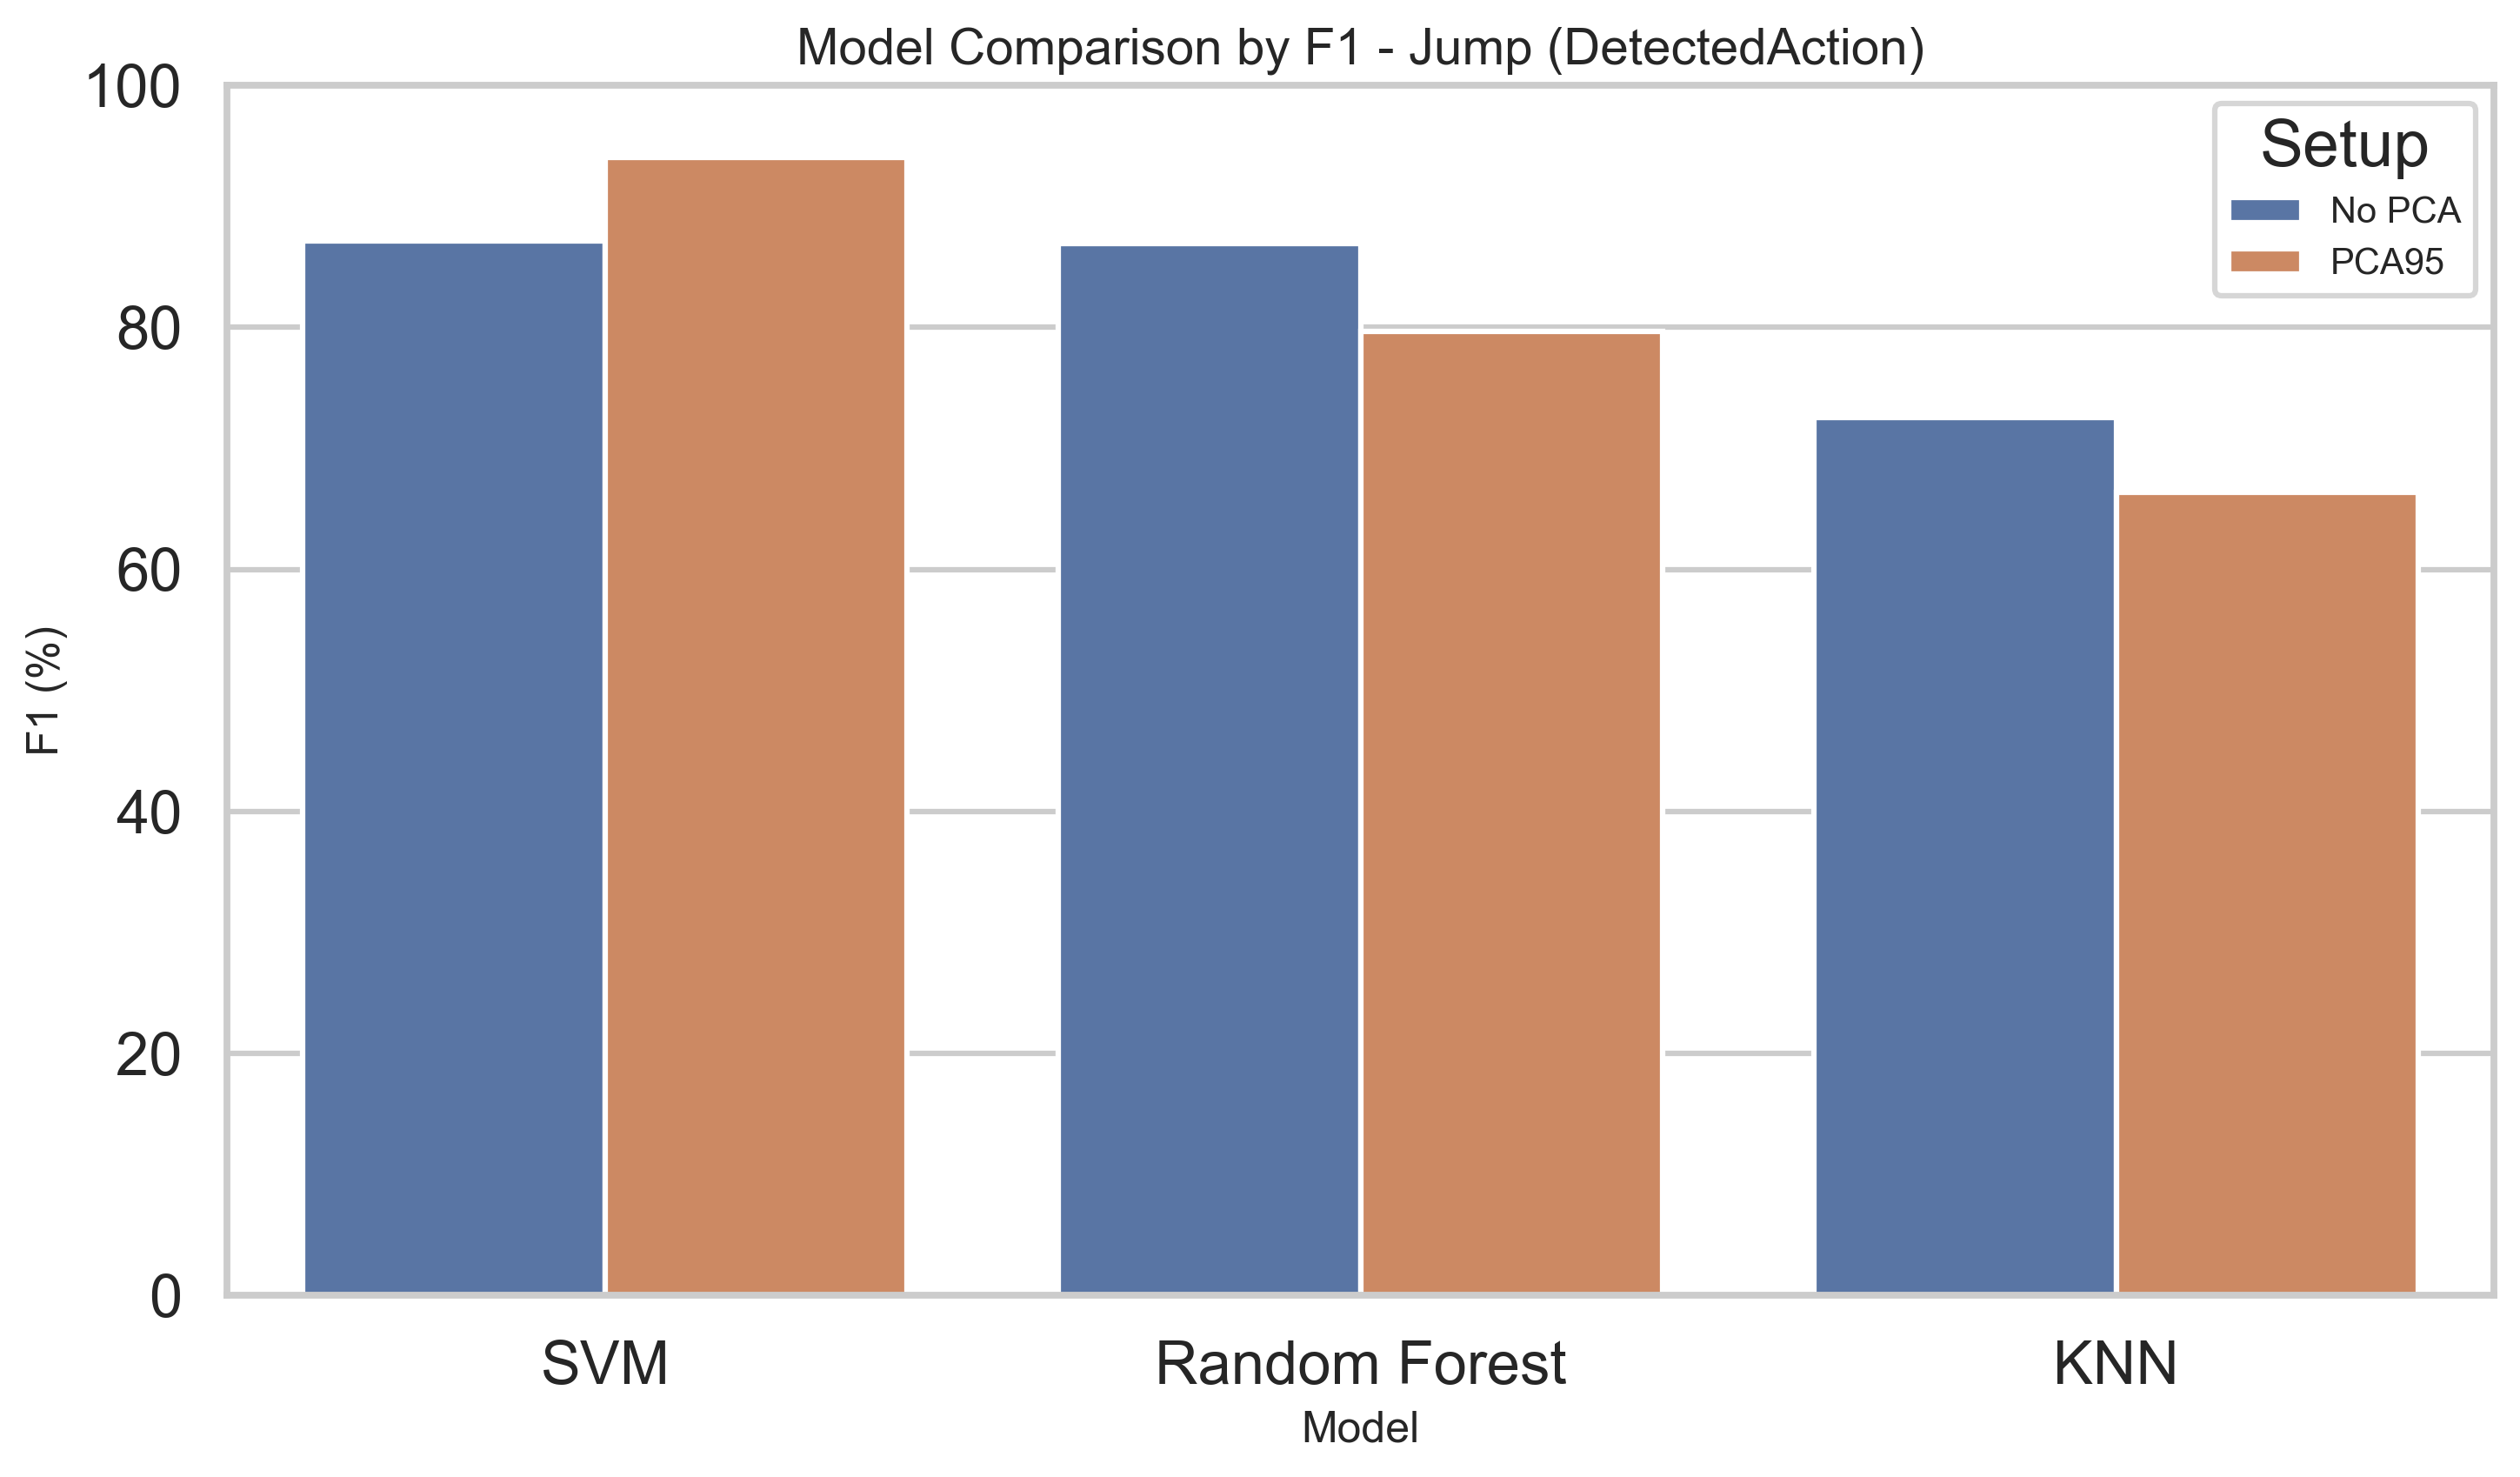
\includegraphics[width=0.85\linewidth]{Images/Generated/TaskResults/Jump/DetectedAction/model_comparison_f1.png}
    \caption{مقایسه عملکرد مدل‌ها بر اساس معیار \lr{F1} در فعالیت پریدن.}
    \label{fig:jump_detectedaction_model_comparison_f1}
\end{figure}

\noindent\textbf{توضیح شکل:} این نمودار اثر استفاده یا عدم استفاده از کاهش بعد را برای هر مدل نشان می‌دهد.
\vspace{0.8em}

\begin{figure}[H]
    \centering
    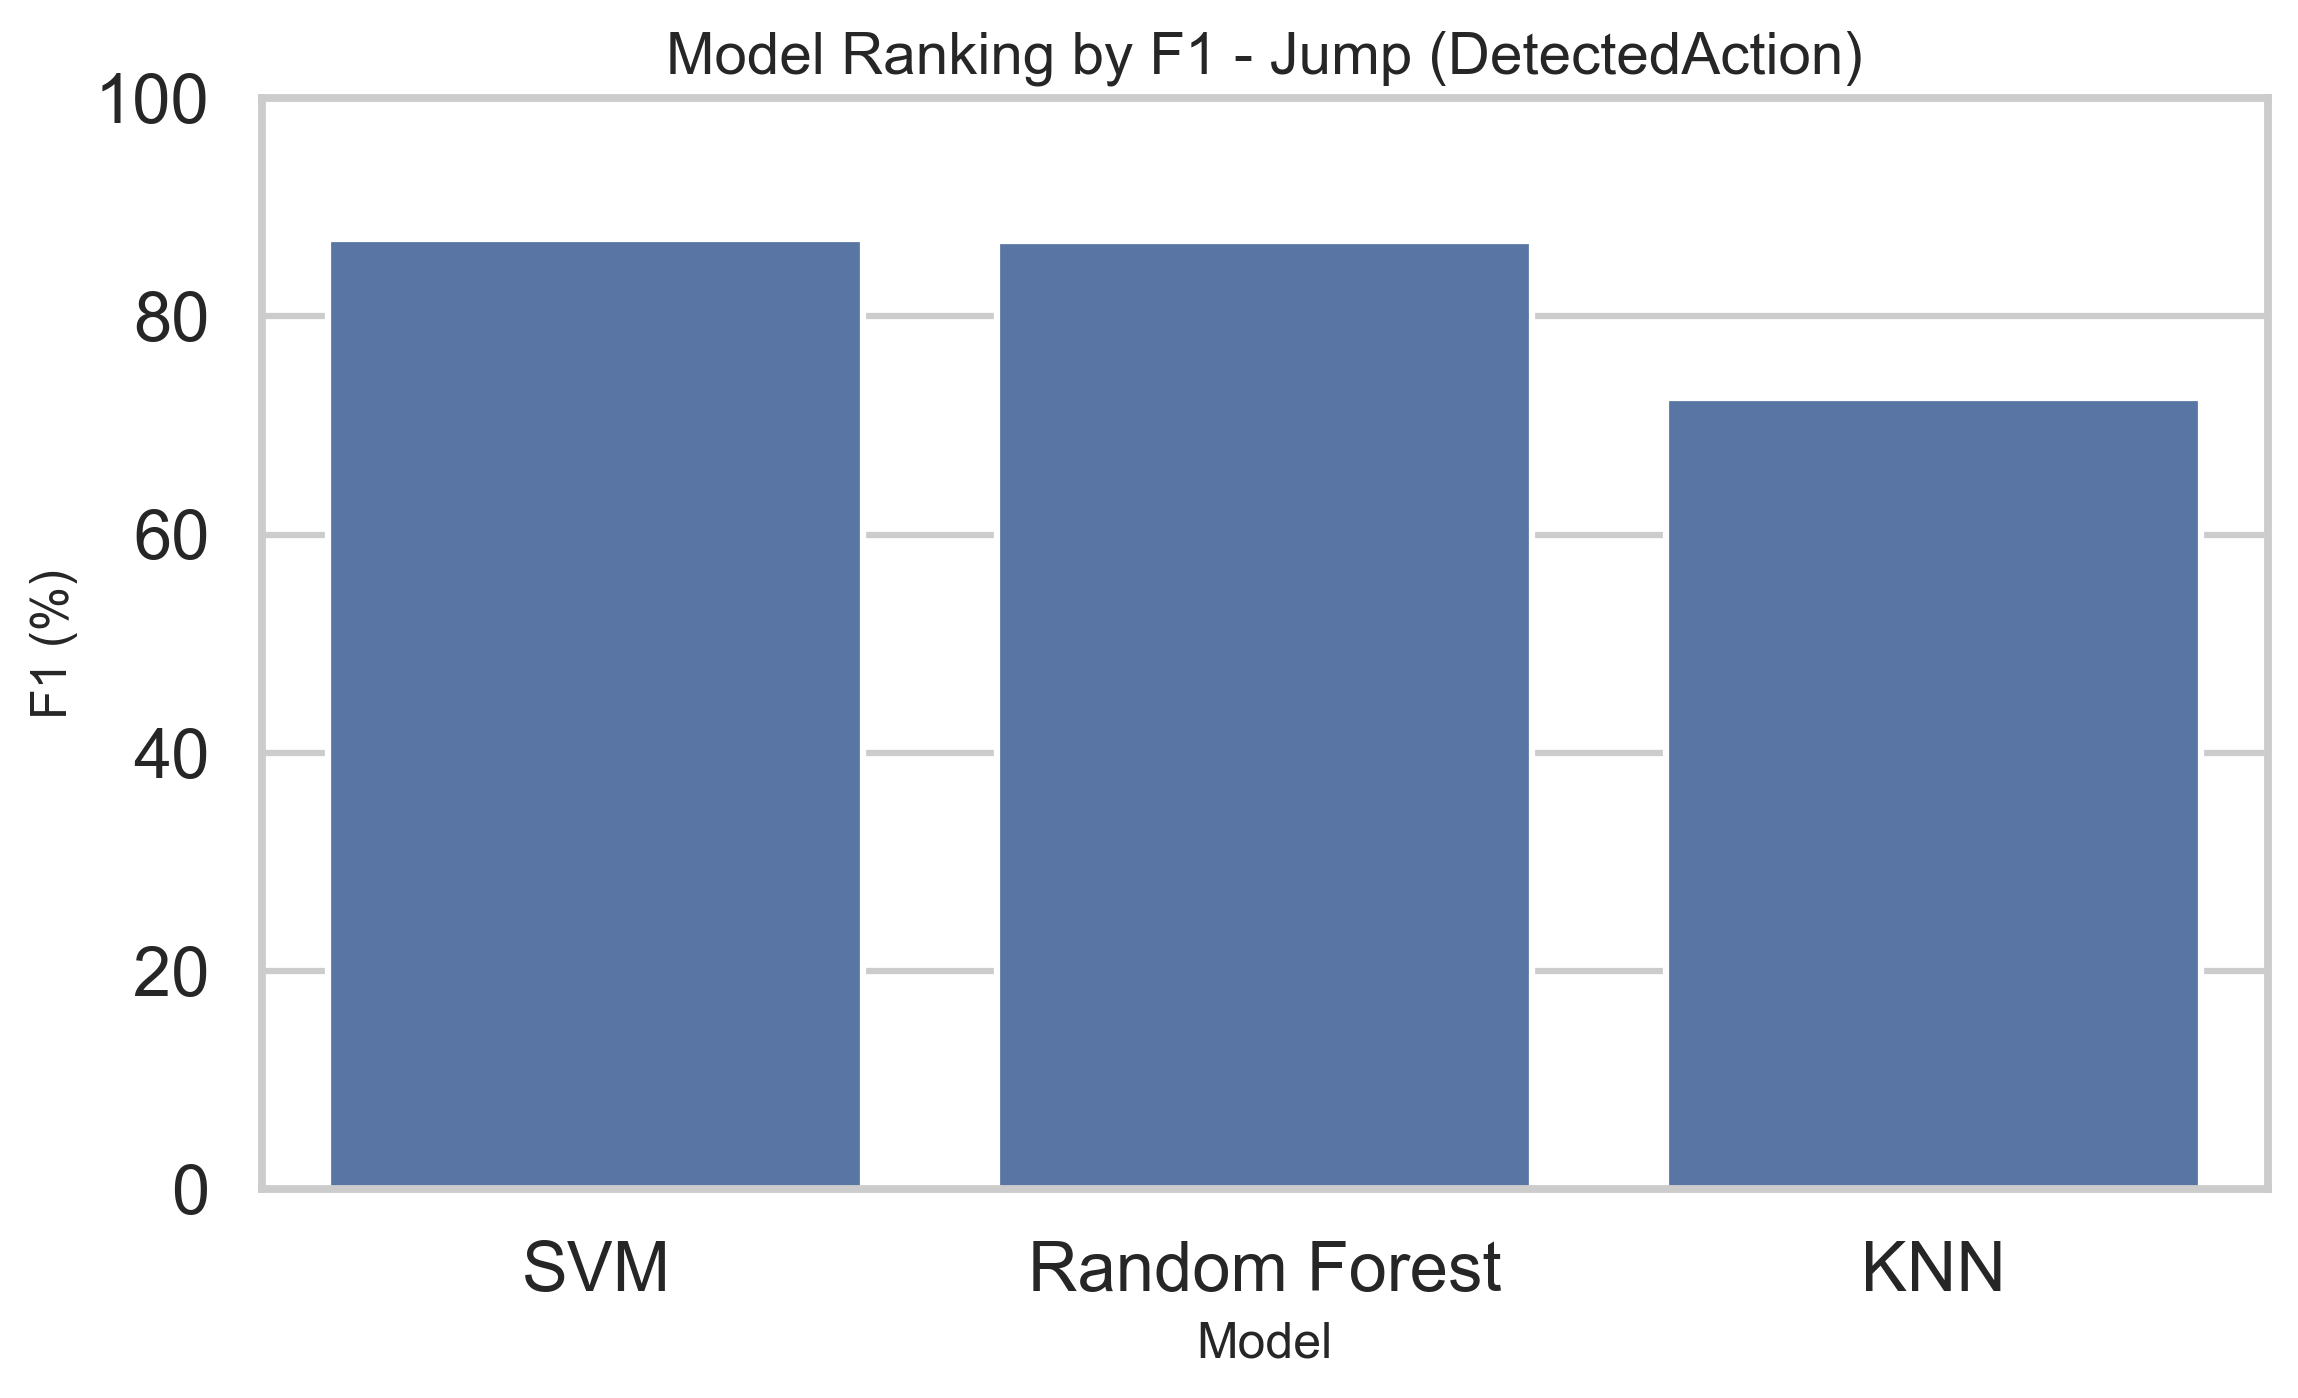
\includegraphics[width=0.85\linewidth]{Images/Generated/TaskResults/Jump/DetectedAction/model_ranking_f1.png}
    \caption{رتبه‌بندی مدل‌ها بر اساس معیار \lr{F1} در فعالیت پریدن.}
    \label{fig:jump_detectedaction_model_ranking_f1}
\end{figure}

\noindent\textbf{توضیح شکل:} این شکل جمع‌بندی سریعی از برتری نسبی مدل‌ها ارائه می‌دهد.
\vspace{0.8em}

\begin{figure}[H]
    \centering
    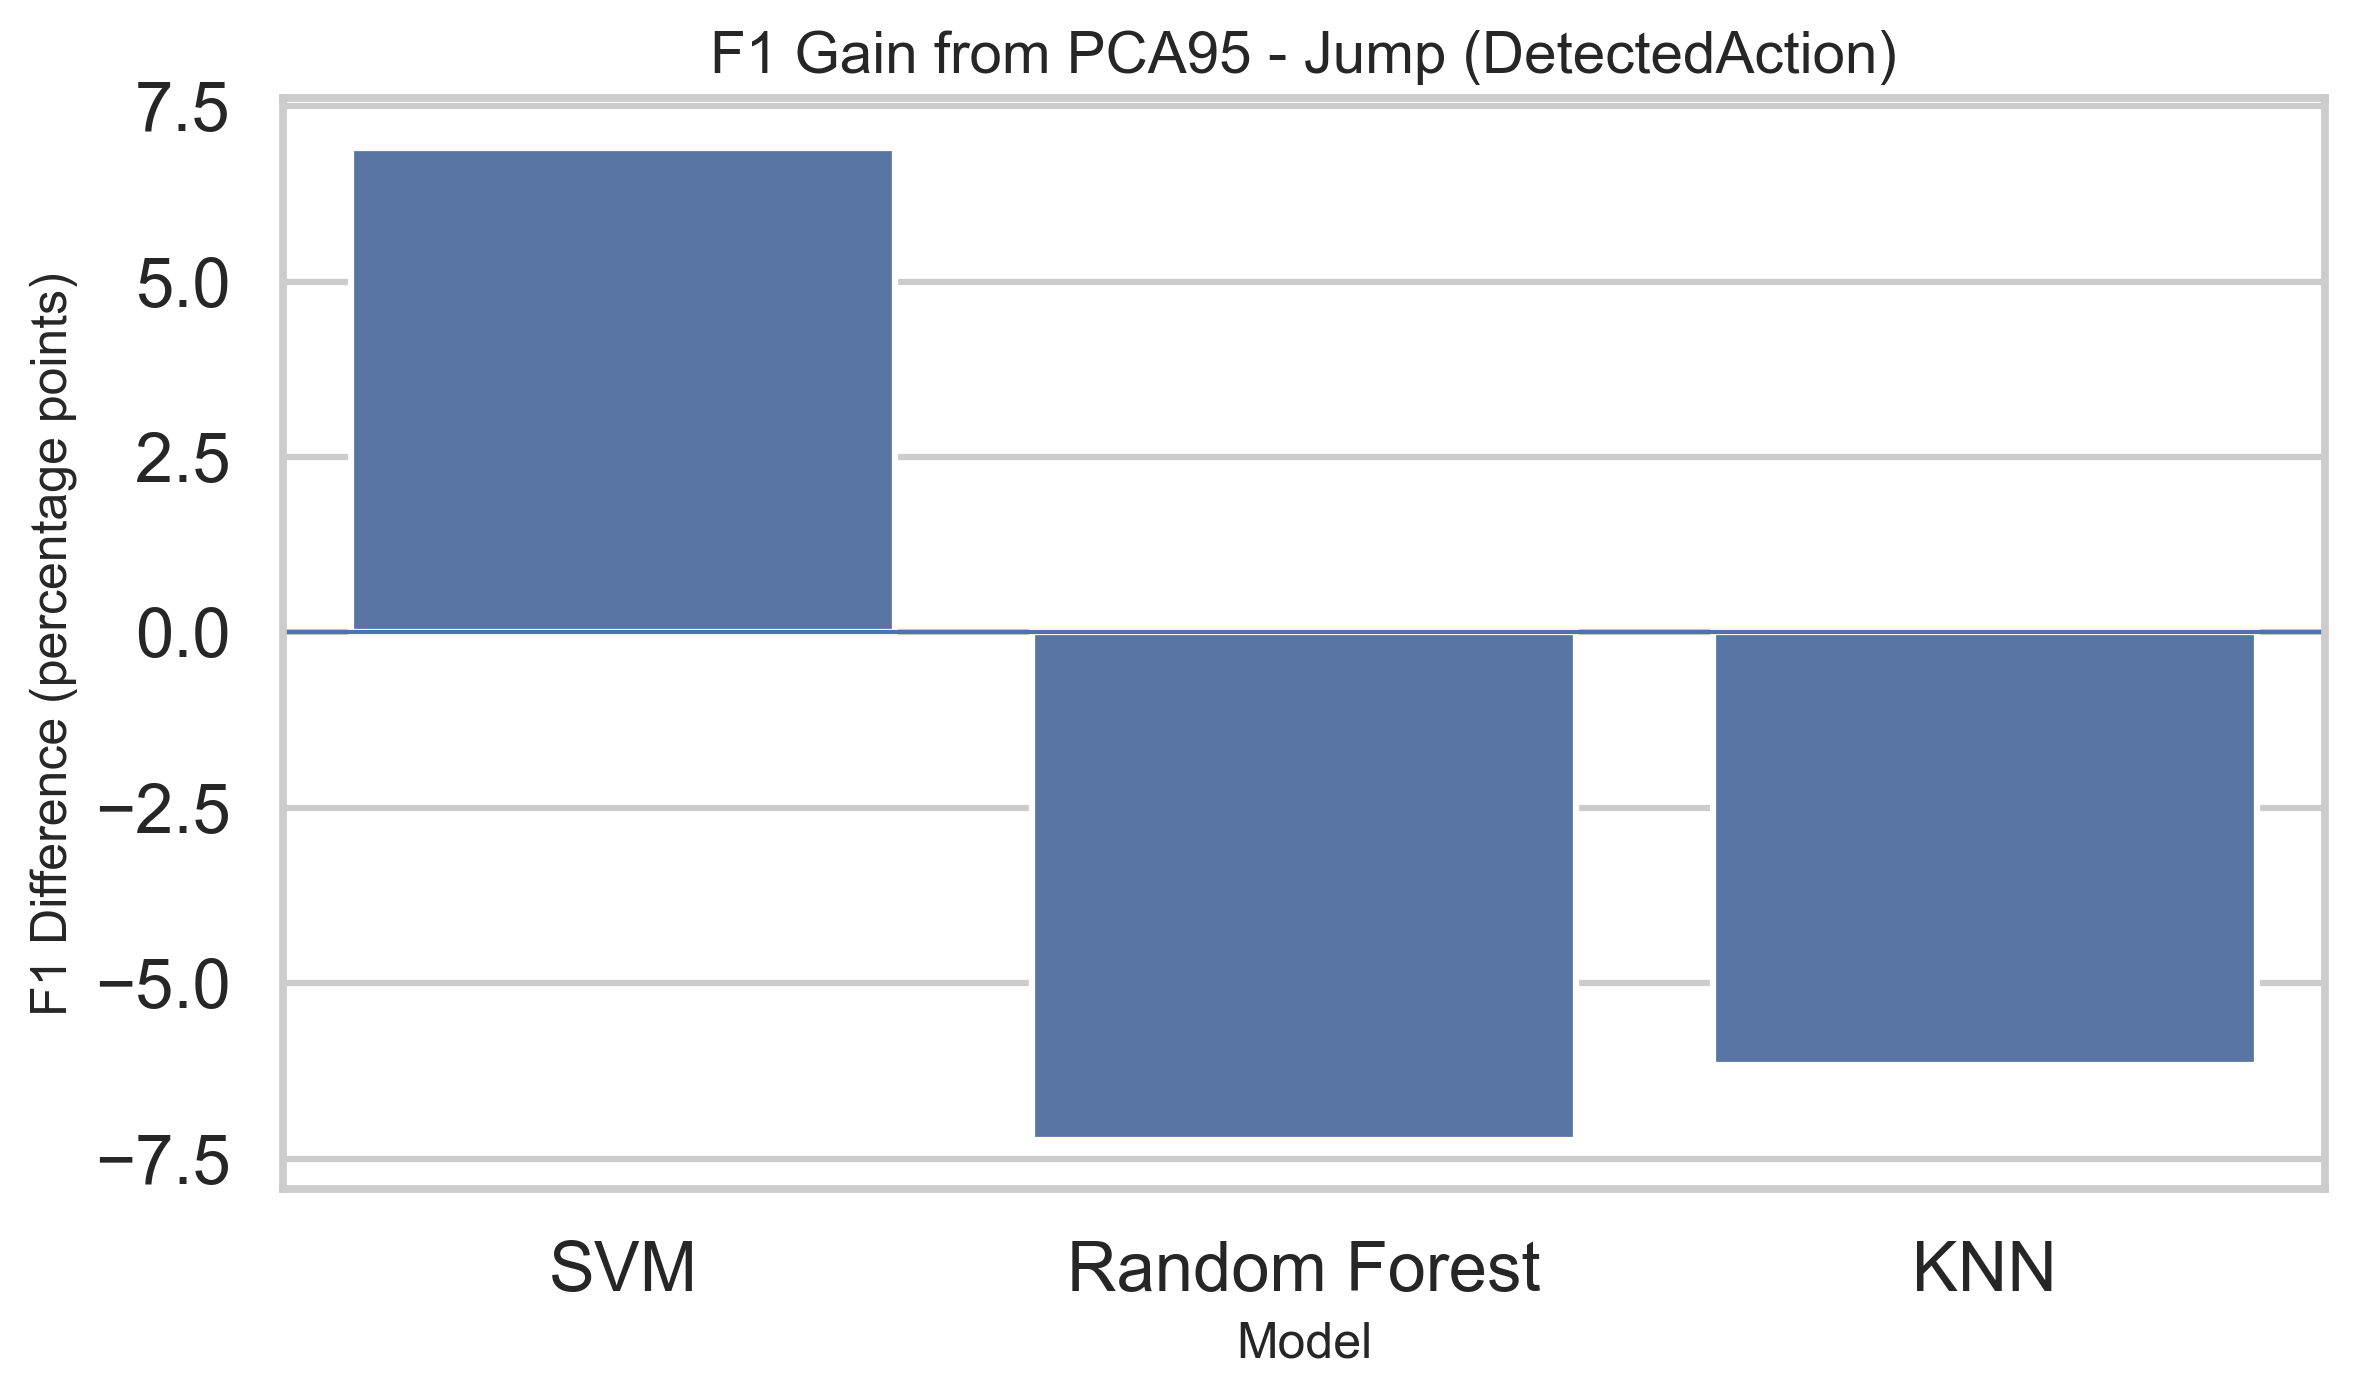
\includegraphics[width=0.85\linewidth]{Images/Generated/TaskResults/Jump/DetectedAction/f1_gain_pca_vs_no_pca.png}
    \caption{تغییر معیار \lr{F1} پس از اعمال \lr{PCA95} در فعالیت پریدن.}
    \label{fig:jump_detectedaction_f1_gain_pca}
\end{figure}

\noindent\textbf{توضیح شکل:} این شکل نشان می‌دهد کاهش بعد برای هر مدل سودمند بوده یا موجب افت عملکرد شده است.
\vspace{0.8em}

\begin{figure}[H]
    \centering
    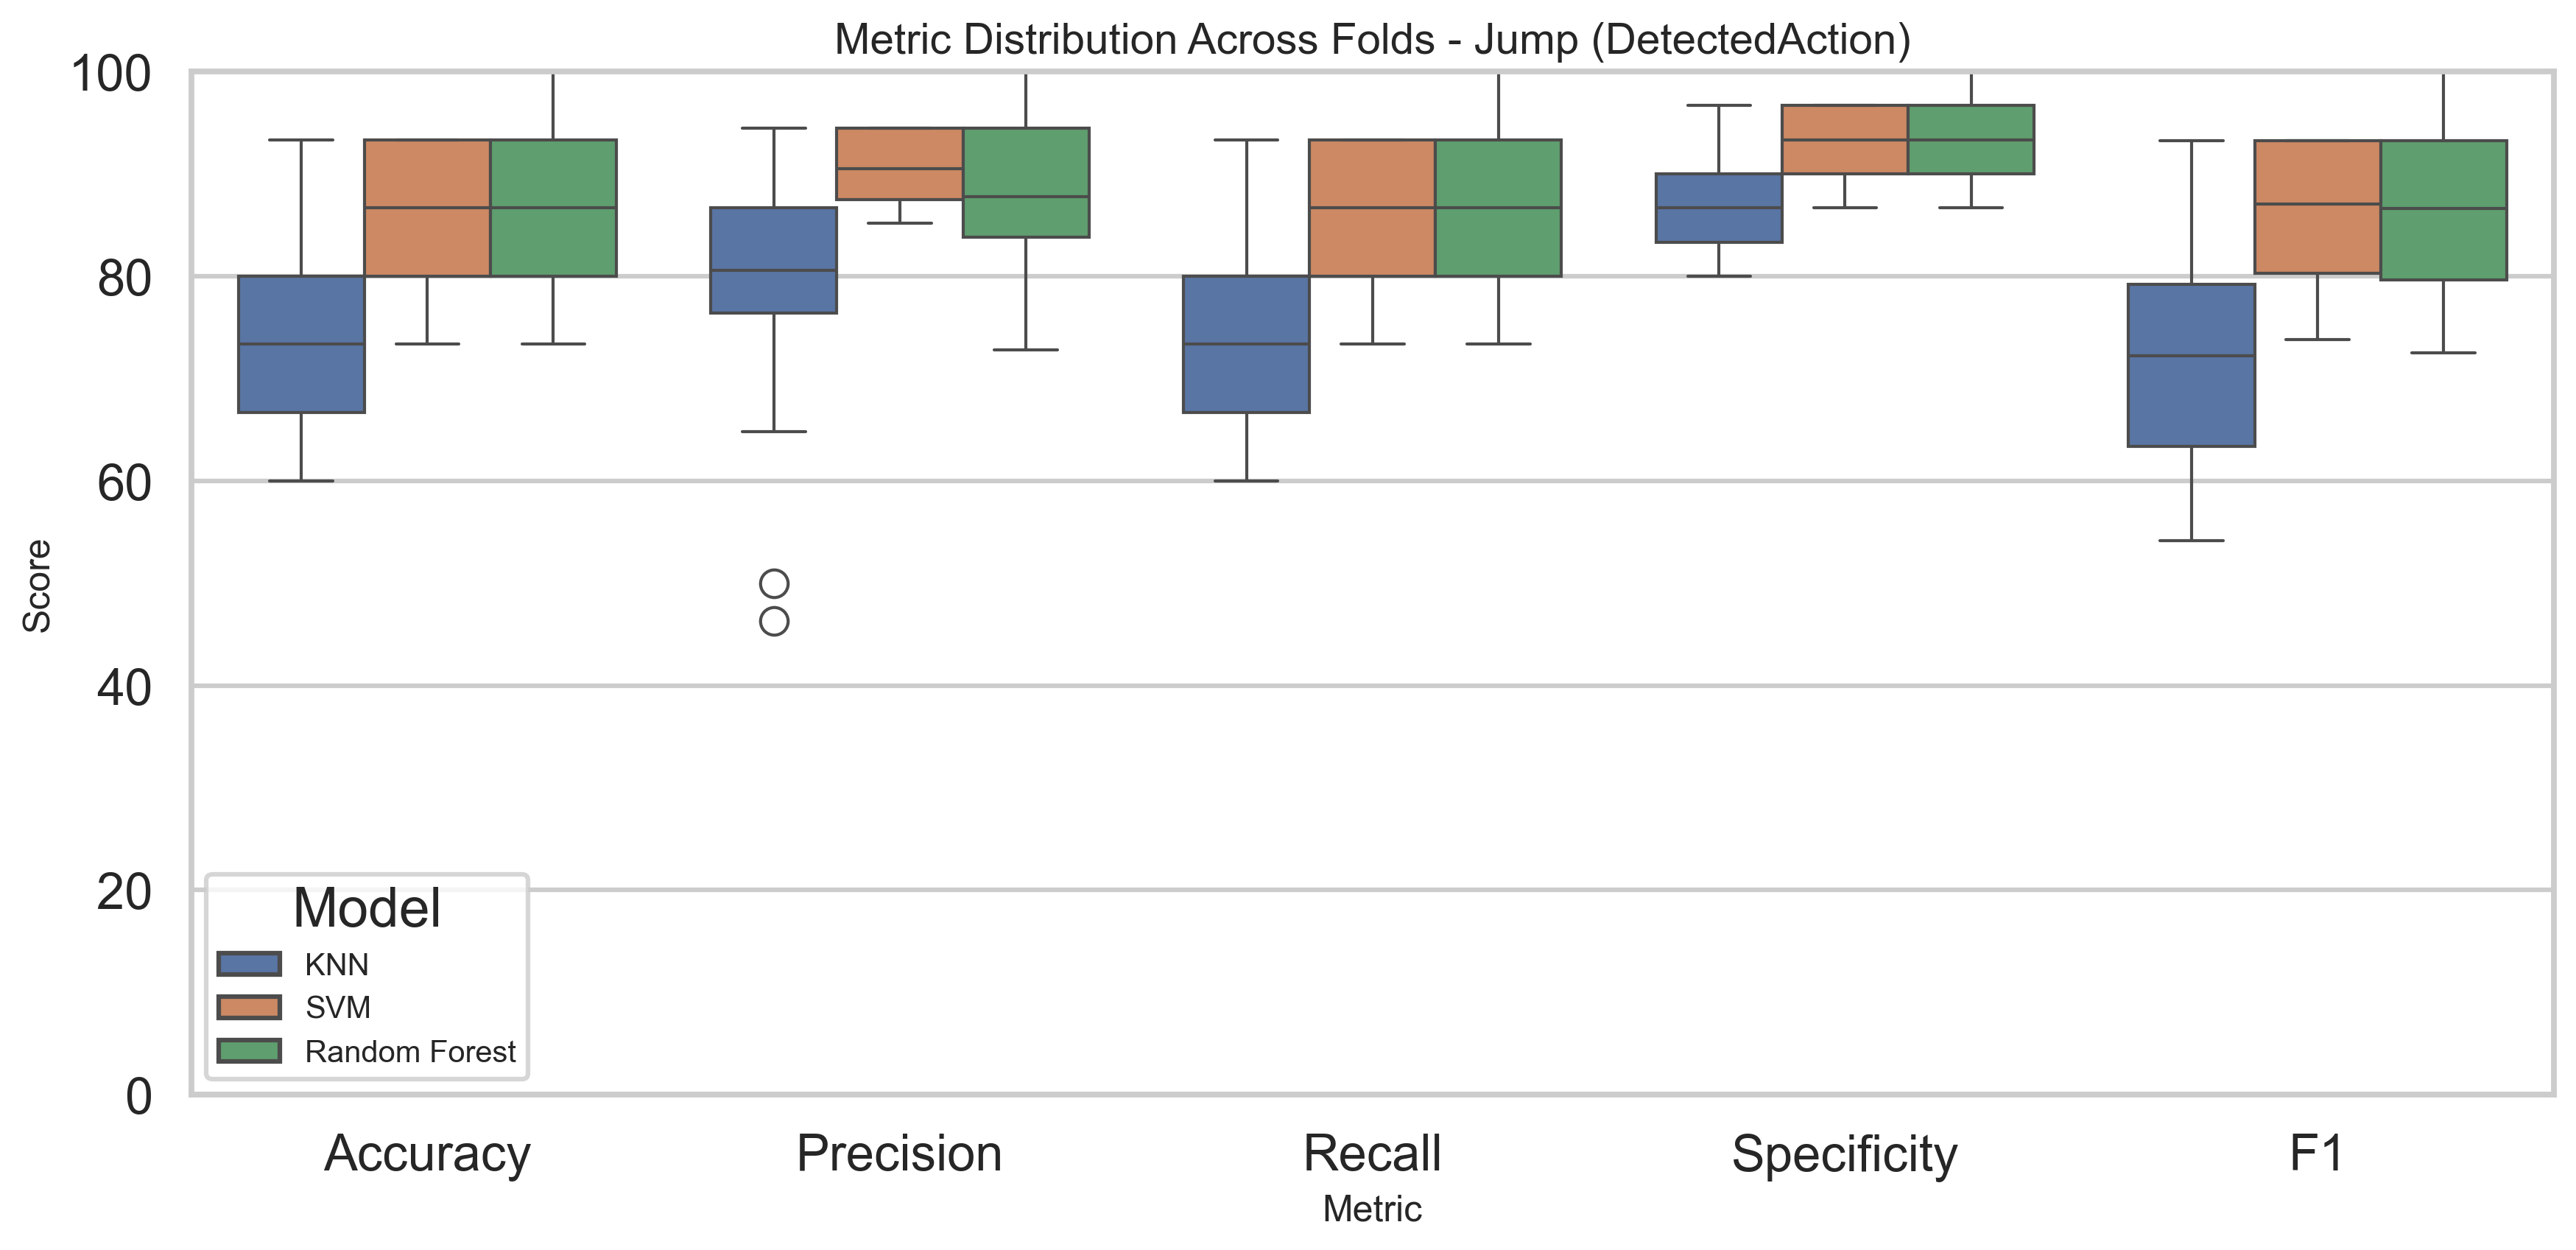
\includegraphics[width=0.85\linewidth]{Images/Generated/TaskResults/Jump/DetectedAction/metric_boxplots.png}
    \caption{پراکندگی معیارهای ارزیابی در تکرارهای اعتبارسنجی برای فعالیت پریدن.}
    \label{fig:jump_detectedaction_metric_boxplots}
\end{figure}

\noindent\textbf{توضیح شکل:} این شکل پایداری مدل‌ها را در foldهای مختلف نشان می‌دهد.
\vspace{0.8em}

\begin{figure}[H]
    \centering
    
\includegraphics[width=0.85\linewidth]{Images/Generated/TaskResults/Jump/DetectedAction/confusion_matrices_no_pca.png}
    \caption{ماتریس درهم‌ریختگی نرمال‌شده مدل‌ها در فعالیت پریدن (no_pca).}
    \label{fig:jump_detectedaction_confusion_no_pca}
\end{figure}

\noindent\textbf{توضیح شکل:} این شکل مشخص می‌کند خطاهای اصلی بین کدام کلاس‌های عملکردی رخ داده است.
\vspace{0.8em}

\begin{figure}[H]
    \centering
    
\includegraphics[width=0.85\linewidth]{Images/Generated/TaskResults/Jump/DetectedAction/per_class_recall_no_pca.png}
    \caption{مقایسه \lr{Recall} هر کلاس در فعالیت پریدن (no_pca).}
    \label{fig:jump_detectedaction_per_class_recall_no_pca}
\end{figure}

\noindent\textbf{توضیح شکل:} این نمودار حساسیت مدل‌ها نسبت به هر سطح عملکردی را نشان می‌دهد.
\vspace{0.8em}

\begin{figure}[H]
    \centering
    
\includegraphics[width=0.85\linewidth]{Images/Generated/TaskResults/Jump/DetectedAction/confusion_matrices_pca95.png}
    \caption{ماتریس درهم‌ریختگی نرمال‌شده مدل‌ها در فعالیت پریدن (pca95).}
    \label{fig:jump_detectedaction_confusion_pca95}
\end{figure}

\noindent\textbf{توضیح شکل:} این شکل مشخص می‌کند خطاهای اصلی بین کدام کلاس‌های عملکردی رخ داده است.
\vspace{0.8em}

\begin{figure}[H]
    \centering
    
\includegraphics[width=0.85\linewidth]{Images/Generated/TaskResults/Jump/DetectedAction/per_class_recall_pca95.png}
    \caption{مقایسه \lr{Recall} هر کلاس در فعالیت پریدن (pca95).}
    \label{fig:jump_detectedaction_per_class_recall_pca95}
\end{figure}

\noindent\textbf{توضیح شکل:} این نمودار حساسیت مدل‌ها نسبت به هر سطح عملکردی را نشان می‌دهد.
\vspace{0.8em}

\begin{figure}[H]
    \centering
    
\includegraphics[width=0.85\linewidth]{Images/Generated/TaskResults/Jump/DetectedAction/rf_top_feature_importance.png}
    \caption{20 ویژگی برتر بر اساس اهمیت در مدل \lr{Random Forest} برای فعالیت پریدن.}
    \label{fig:jump_detectedaction_rf_importance}
\end{figure}

\noindent\textbf{توضیح شکل:} این شکل نشان می‌دهد کدام حسگرها، محورها و شاخص‌های آماری نقش بیشتری در تصمیم‌گیری مدل داشته‌اند.
\vspace{0.8em}

\begin{figure}[H]
    \centering
    
\includegraphics[width=0.85\linewidth]{Images/Generated/TaskResults/Jump/DetectedAction/class_centroid_feature_heatmap.png}
    \caption{میانگین نرمال‌شده ویژگی‌های برتر در کلاس‌های مختلف فعالیت پریدن.}
    \label{fig:jump_detectedaction_class_centroid_heatmap}
\end{figure}

\noindent\textbf{توضیح شکل:} این نقشه حرارتی الگوی میانگین ویژگی‌ها را در هر سطح عملکردی نمایش می‌دهد.
\vspace{0.8em}

\begin{figure}[H]
    \centering
    
\includegraphics[width=0.85\linewidth]{Images/Generated/TaskResults/Jump/DetectedAction/svm_metrics_vs_pca_components.png}
    \caption{تغییر عملکرد مدل \lr{SVM} نسبت به تعداد مؤلفه‌های اصلی در فعالیت پریدن.}
    \label{fig:jump_detectedaction_svm_metrics_vs_pca_components}
\end{figure}

\noindent\textbf{توضیح شکل:} این نمودار برای انتخاب بازه مناسب تعداد مؤلفه‌های اصلی استفاده می‌شود.
\vspace{0.8em}

\begin{figure}[H]
    \centering
    
\includegraphics[width=0.85\linewidth]{Images/Generated/TaskResults/Jump/DetectedAction/models_f1_vs_pca_components.png}
    \caption{مقایسه مدل‌ها نسبت به تعداد مؤلفه‌های اصلی در فعالیت پریدن.}
    \label{fig:jump_detectedaction_models_f1_vs_pca_components}
\end{figure}

\noindent\textbf{توضیح شکل:} این نمودار نشان می‌دهد انتخاب تعداد مؤلفه‌ها و انتخاب مدل باید هم‌زمان انجام شود.
\vspace{0.8em}


\subsection*{نمودارهای فعالیت ایستادن}

\subsubsection*{داده‌های اصلی}

\begin{figure}[H]
    \centering
    
\includegraphics[width=0.85\linewidth]{Images/Generated/TaskResults/Stand/Normal/signal_sample.png}
    \caption{نمونه سیگنال‌های ثبت‌شده در فعالیت ایستادن (داده‌های اصلی).}
    \label{fig:stand_normal_signal_sample}
\end{figure}

\noindent\textbf{توضیح شکل:} این شکل نمایی از ماهیت زمانی سیگنال‌های حسگرها را برای فعالیت مورد نظر نشان می‌دهد.
\vspace{0.8em}

\begin{figure}[H]
    \centering
    
\includegraphics[width=0.85\linewidth]{Images/Generated/TaskResults/Stand/Normal/class_distribution.png}
    \caption{توزیع تعداد نمونه‌ها در سطوح عملکردی فعالیت ایستادن.}
    \label{fig:stand_normal_class_distribution}
\end{figure}

\noindent\textbf{توضیح شکل:} این نمودار برای بررسی تعادل داده‌ها بین کلاس‌های صفر، یک و دو استفاده می‌شود.
\vspace{0.8em}

\begin{figure}[H]
    \centering
    
\includegraphics[width=0.85\linewidth]{Images/Generated/TaskResults/Stand/Normal/feature_correlation_heatmap.png}
    \caption{نقشه همبستگی 20 ویژگی با بیشترین واریانس در فعالیت ایستادن.}
    \label{fig:stand_normal_feature_correlation}
\end{figure}

\noindent\textbf{توضیح شکل:} این نمودار وجود اطلاعات تکراری در فضای ویژگی را نشان می‌دهد و استفاده از کاهش بعد را توجیه می‌کند.
\vspace{0.8em}

\begin{figure}[H]
    \centering
    
\includegraphics[width=0.85\linewidth]{Images/Generated/TaskResults/Stand/Normal/pca_variance_curve.png}
    \caption{درصد واریانس توضیح‌داده‌شده و واریانس تجمعی مؤلفه‌های اصلی در فعالیت ایستادن.}
    \label{fig:stand_normal_pca_variance}
\end{figure}

\noindent\textbf{توضیح شکل:} این شکل مبنای انتخاب آستانه ۹۵ درصد و تعیین تعداد مؤلفه‌های نگه‌داشته‌شده را نشان می‌دهد.
\vspace{0.8em}

\begin{figure}[H]
    \centering
    
\includegraphics[width=0.85\linewidth]{Images/Generated/TaskResults/Stand/Normal/pca_scatter_pc1_pc2.png}
    \caption{پراکندگی نمونه‌های فعالیت ایستادن در فضای دو مؤلفه اصلی اول.}
    \label{fig:stand_normal_pca_scatter}
\end{figure}

\noindent\textbf{توضیح شکل:} این شکل یک تصویر اولیه از جدایی یا هم‌پوشانی کلاس‌ها در فضای کاهش‌یافته ارائه می‌دهد.
\vspace{0.8em}

\begin{figure}[H]
    \centering
    
\includegraphics[width=0.85\linewidth]{Images/Generated/TaskResults/Stand/Normal/model_comparison_f1.png}
    \caption{مقایسه عملکرد مدل‌ها بر اساس معیار \lr{F1} در فعالیت ایستادن.}
    \label{fig:stand_normal_model_comparison_f1}
\end{figure}

\noindent\textbf{توضیح شکل:} این نمودار اثر استفاده یا عدم استفاده از کاهش بعد را برای هر مدل نشان می‌دهد.
\vspace{0.8em}

\begin{figure}[H]
    \centering
    
\includegraphics[width=0.85\linewidth]{Images/Generated/TaskResults/Stand/Normal/model_ranking_f1.png}
    \caption{رتبه‌بندی مدل‌ها بر اساس معیار \lr{F1} در فعالیت ایستادن.}
    \label{fig:stand_normal_model_ranking_f1}
\end{figure}

\noindent\textbf{توضیح شکل:} این شکل جمع‌بندی سریعی از برتری نسبی مدل‌ها ارائه می‌دهد.
\vspace{0.8em}

\begin{figure}[H]
    \centering
    
\includegraphics[width=0.85\linewidth]{Images/Generated/TaskResults/Stand/Normal/f1_gain_pca_vs_no_pca.png}
    \caption{تغییر معیار \lr{F1} پس از اعمال \lr{PCA95} در فعالیت ایستادن.}
    \label{fig:stand_normal_f1_gain_pca}
\end{figure}

\noindent\textbf{توضیح شکل:} این شکل نشان می‌دهد کاهش بعد برای هر مدل سودمند بوده یا موجب افت عملکرد شده است.
\vspace{0.8em}

\begin{figure}[H]
    \centering
    
\includegraphics[width=0.85\linewidth]{Images/Generated/TaskResults/Stand/Normal/metric_boxplots.png}
    \caption{پراکندگی معیارهای ارزیابی در تکرارهای اعتبارسنجی برای فعالیت ایستادن.}
    \label{fig:stand_normal_metric_boxplots}
\end{figure}

\noindent\textbf{توضیح شکل:} این شکل پایداری مدل‌ها را در foldهای مختلف نشان می‌دهد.
\vspace{0.8em}

\begin{figure}[H]
    \centering
    
\includegraphics[width=0.85\linewidth]{Images/Generated/TaskResults/Stand/Normal/confusion_matrices_no_pca.png}
    \caption{ماتریس درهم‌ریختگی نرمال‌شده مدل‌ها در فعالیت ایستادن (no_pca).}
    \label{fig:stand_normal_confusion_no_pca}
\end{figure}

\noindent\textbf{توضیح شکل:} این شکل مشخص می‌کند خطاهای اصلی بین کدام کلاس‌های عملکردی رخ داده است.
\vspace{0.8em}

\begin{figure}[H]
    \centering
    
\includegraphics[width=0.85\linewidth]{Images/Generated/TaskResults/Stand/Normal/per_class_recall_no_pca.png}
    \caption{مقایسه \lr{Recall} هر کلاس در فعالیت ایستادن (no_pca).}
    \label{fig:stand_normal_per_class_recall_no_pca}
\end{figure}

\noindent\textbf{توضیح شکل:} این نمودار حساسیت مدل‌ها نسبت به هر سطح عملکردی را نشان می‌دهد.
\vspace{0.8em}

\begin{figure}[H]
    \centering
    
\includegraphics[width=0.85\linewidth]{Images/Generated/TaskResults/Stand/Normal/confusion_matrices_pca95.png}
    \caption{ماتریس درهم‌ریختگی نرمال‌شده مدل‌ها در فعالیت ایستادن (pca95).}
    \label{fig:stand_normal_confusion_pca95}
\end{figure}

\noindent\textbf{توضیح شکل:} این شکل مشخص می‌کند خطاهای اصلی بین کدام کلاس‌های عملکردی رخ داده است.
\vspace{0.8em}

\begin{figure}[H]
    \centering
    
\includegraphics[width=0.85\linewidth]{Images/Generated/TaskResults/Stand/Normal/per_class_recall_pca95.png}
    \caption{مقایسه \lr{Recall} هر کلاس در فعالیت ایستادن (pca95).}
    \label{fig:stand_normal_per_class_recall_pca95}
\end{figure}

\noindent\textbf{توضیح شکل:} این نمودار حساسیت مدل‌ها نسبت به هر سطح عملکردی را نشان می‌دهد.
\vspace{0.8em}

\begin{figure}[H]
    \centering
    
\includegraphics[width=0.85\linewidth]{Images/Generated/TaskResults/Stand/Normal/rf_top_feature_importance.png}
    \caption{20 ویژگی برتر بر اساس اهمیت در مدل \lr{Random Forest} برای فعالیت ایستادن.}
    \label{fig:stand_normal_rf_importance}
\end{figure}

\noindent\textbf{توضیح شکل:} این شکل نشان می‌دهد کدام حسگرها، محورها و شاخص‌های آماری نقش بیشتری در تصمیم‌گیری مدل داشته‌اند.
\vspace{0.8em}

\begin{figure}[H]
    \centering
    
\includegraphics[width=0.85\linewidth]{Images/Generated/TaskResults/Stand/Normal/class_centroid_feature_heatmap.png}
    \caption{میانگین نرمال‌شده ویژگی‌های برتر در کلاس‌های مختلف فعالیت ایستادن.}
    \label{fig:stand_normal_class_centroid_heatmap}
\end{figure}

\noindent\textbf{توضیح شکل:} این نقشه حرارتی الگوی میانگین ویژگی‌ها را در هر سطح عملکردی نمایش می‌دهد.
\vspace{0.8em}

\begin{figure}[H]
    \centering
    
\includegraphics[width=0.85\linewidth]{Images/Generated/TaskResults/Stand/Normal/svm_metrics_vs_pca_components.png}
    \caption{تغییر عملکرد مدل \lr{SVM} نسبت به تعداد مؤلفه‌های اصلی در فعالیت ایستادن.}
    \label{fig:stand_normal_svm_metrics_vs_pca_components}
\end{figure}

\noindent\textbf{توضیح شکل:} این نمودار برای انتخاب بازه مناسب تعداد مؤلفه‌های اصلی استفاده می‌شود.
\vspace{0.8em}

\begin{figure}[H]
    \centering
    
\includegraphics[width=0.85\linewidth]{Images/Generated/TaskResults/Stand/Normal/models_f1_vs_pca_components.png}
    \caption{مقایسه مدل‌ها نسبت به تعداد مؤلفه‌های اصلی در فعالیت ایستادن.}
    \label{fig:stand_normal_models_f1_vs_pca_components}
\end{figure}

\noindent\textbf{توضیح شکل:} این نمودار نشان می‌دهد انتخاب تعداد مؤلفه‌ها و انتخاب مدل باید هم‌زمان انجام شود.
\vspace{0.8em}

\subsection*{نمودارهای فعالیت بلند شدن از صندلی}

\subsubsection*{داده‌های اصلی}

\begin{figure}[H]
    \centering
    
\includegraphics[width=0.85\linewidth]{Images/Generated/TaskResults/Sit_To_Stand/Normal/signal_sample.png}
    \caption{نمونه سیگنال‌های ثبت‌شده در فعالیت بلند شدن از صندلی (داده‌های اصلی).}
    \label{fig:sit_to_stand_normal_signal_sample}
\end{figure}

\noindent\textbf{توضیح شکل:} این شکل نمایی از ماهیت زمانی سیگنال‌های حسگرها را برای فعالیت مورد نظر نشان می‌دهد.
\vspace{0.8em}

\begin{figure}[H]
    \centering
    
\includegraphics[width=0.85\linewidth]{Images/Generated/TaskResults/Sit_To_Stand/Normal/class_distribution.png}
    \caption{توزیع تعداد نمونه‌ها در سطوح عملکردی فعالیت بلند شدن از صندلی.}
    \label{fig:sit_to_stand_normal_class_distribution}
\end{figure}

\noindent\textbf{توضیح شکل:} این نمودار برای بررسی تعادل داده‌ها بین کلاس‌های صفر، یک و دو استفاده می‌شود.
\vspace{0.8em}

\begin{figure}[H]
    \centering
    
\includegraphics[width=0.85\linewidth]{Images/Generated/TaskResults/Sit_To_Stand/Normal/feature_correlation_heatmap.png}
    \caption{نقشه همبستگی 20 ویژگی با بیشترین واریانس در فعالیت بلند شدن از صندلی.}
    \label{fig:sit_to_stand_normal_feature_correlation}
\end{figure}

\noindent\textbf{توضیح شکل:} این نمودار وجود اطلاعات تکراری در فضای ویژگی را نشان می‌دهد و استفاده از کاهش بعد را توجیه می‌کند.
\vspace{0.8em}

\begin{figure}[H]
    \centering
    
\includegraphics[width=0.85\linewidth]{Images/Generated/TaskResults/Sit_To_Stand/Normal/pca_variance_curve.png}
    \caption{درصد واریانس توضیح‌داده‌شده و واریانس تجمعی مؤلفه‌های اصلی در فعالیت بلند شدن از صندلی.}
    \label{fig:sit_to_stand_normal_pca_variance}
\end{figure}

\noindent\textbf{توضیح شکل:} این شکل مبنای انتخاب آستانه ۹۵ درصد و تعیین تعداد مؤلفه‌های نگه‌داشته‌شده را نشان می‌دهد.
\vspace{0.8em}

\begin{figure}[H]
    \centering
    
\includegraphics[width=0.85\linewidth]{Images/Generated/TaskResults/Sit_To_Stand/Normal/pca_scatter_pc1_pc2.png}
    \caption{پراکندگی نمونه‌های فعالیت بلند شدن از صندلی در فضای دو مؤلفه اصلی اول.}
    \label{fig:sit_to_stand_normal_pca_scatter}
\end{figure}

\noindent\textbf{توضیح شکل:} این شکل یک تصویر اولیه از جدایی یا هم‌پوشانی کلاس‌ها در فضای کاهش‌یافته ارائه می‌دهد.
\vspace{0.8em}

\begin{figure}[H]
    \centering
    
\includegraphics[width=0.85\linewidth]{Images/Generated/TaskResults/Sit_To_Stand/Normal/model_comparison_f1.png}
    \caption{مقایسه عملکرد مدل‌ها بر اساس معیار \lr{F1} در فعالیت بلند شدن از صندلی.}
    \label{fig:sit_to_stand_normal_model_comparison_f1}
\end{figure}

\noindent\textbf{توضیح شکل:} این نمودار اثر استفاده یا عدم استفاده از کاهش بعد را برای هر مدل نشان می‌دهد.
\vspace{0.8em}

\begin{figure}[H]
    \centering
    
\includegraphics[width=0.85\linewidth]{Images/Generated/TaskResults/Sit_To_Stand/Normal/model_ranking_f1.png}
    \caption{رتبه‌بندی مدل‌ها بر اساس معیار \lr{F1} در فعالیت بلند شدن از صندلی.}
    \label{fig:sit_to_stand_normal_model_ranking_f1}
\end{figure}

\noindent\textbf{توضیح شکل:} این شکل جمع‌بندی سریعی از برتری نسبی مدل‌ها ارائه می‌دهد.
\vspace{0.8em}

\begin{figure}[H]
    \centering
    
\includegraphics[width=0.85\linewidth]{Images/Generated/TaskResults/Sit_To_Stand/Normal/f1_gain_pca_vs_no_pca.png}
    \caption{تغییر معیار \lr{F1} پس از اعمال \lr{PCA95} در فعالیت بلند شدن از صندلی.}
    \label{fig:sit_to_stand_normal_f1_gain_pca}
\end{figure}

\noindent\textbf{توضیح شکل:} این شکل نشان می‌دهد کاهش بعد برای هر مدل سودمند بوده یا موجب افت عملکرد شده است.
\vspace{0.8em}

\begin{figure}[H]
    \centering
    
\includegraphics[width=0.85\linewidth]{Images/Generated/TaskResults/Sit_To_Stand/Normal/metric_boxplots.png}
    \caption{پراکندگی معیارهای ارزیابی در تکرارهای اعتبارسنجی برای فعالیت بلند شدن از صندلی.}
    \label{fig:sit_to_stand_normal_metric_boxplots}
\end{figure}

\noindent\textbf{توضیح شکل:} این شکل پایداری مدل‌ها را در foldهای مختلف نشان می‌دهد.
\vspace{0.8em}

\begin{figure}[H]
    \centering
    
\includegraphics[width=0.85\linewidth]{Images/Generated/TaskResults/Sit_To_Stand/Normal/confusion_matrices_no_pca.png}
    \caption{ماتریس درهم‌ریختگی نرمال‌شده مدل‌ها در فعالیت بلند شدن از صندلی (no_pca).}
    \label{fig:sit_to_stand_normal_confusion_no_pca}
\end{figure}

\noindent\textbf{توضیح شکل:} این شکل مشخص می‌کند خطاهای اصلی بین کدام کلاس‌های عملکردی رخ داده است.
\vspace{0.8em}

\begin{figure}[H]
    \centering
    
\includegraphics[width=0.85\linewidth]{Images/Generated/TaskResults/Sit_To_Stand/Normal/per_class_recall_no_pca.png}
    \caption{مقایسه \lr{Recall} هر کلاس در فعالیت بلند شدن از صندلی (no_pca).}
    \label{fig:sit_to_stand_normal_per_class_recall_no_pca}
\end{figure}

\noindent\textbf{توضیح شکل:} این نمودار حساسیت مدل‌ها نسبت به هر سطح عملکردی را نشان می‌دهد.
\vspace{0.8em}

\begin{figure}[H]
    \centering
    
\includegraphics[width=0.85\linewidth]{Images/Generated/TaskResults/Sit_To_Stand/Normal/confusion_matrices_pca95.png}
    \caption{ماتریس درهم‌ریختگی نرمال‌شده مدل‌ها در فعالیت بلند شدن از صندلی (pca95).}
    \label{fig:sit_to_stand_normal_confusion_pca95}
\end{figure}

\noindent\textbf{توضیح شکل:} این شکل مشخص می‌کند خطاهای اصلی بین کدام کلاس‌های عملکردی رخ داده است.
\vspace{0.8em}

\begin{figure}[H]
    \centering
    
\includegraphics[width=0.85\linewidth]{Images/Generated/TaskResults/Sit_To_Stand/Normal/per_class_recall_pca95.png}
    \caption{مقایسه \lr{Recall} هر کلاس در فعالیت بلند شدن از صندلی (pca95).}
    \label{fig:sit_to_stand_normal_per_class_recall_pca95}
\end{figure}

\noindent\textbf{توضیح شکل:} این نمودار حساسیت مدل‌ها نسبت به هر سطح عملکردی را نشان می‌دهد.
\vspace{0.8em}

\begin{figure}[H]
    \centering
    \includegraphics[width=0.85\linewidth]{Images/Generated/TaskResults/Sit_To_Stand/Normal/rf_top_feature_importance.png}
    \caption{20 ویژگی برتر بر اساس اهمیت در مدل \lr{Random Forest} برای فعالیت بلند شدن از صندلی.}
    \label{fig:sit_to_stand_normal_rf_importance}
\end{figure}

\noindent\textbf{توضیح شکل:} این شکل نشان می‌دهد کدام حسگرها، محورها و شاخص‌های آماری نقش بیشتری در تصمیم‌گیری مدل داشته‌اند.
\vspace{0.8em}

\begin{figure}[H]
    \centering
    \includegraphics[width=0.85\linewidth]{Images/Generated/TaskResults/Sit_To_Stand/Normal/class_centroid_feature_heatmap.png}
    \caption{میانگین نرمال‌شده ویژگی‌های برتر در کلاس‌های مختلف فعالیت بلند شدن از صندلی.}
    \label{fig:sit_to_stand_normal_class_centroid_heatmap}
\end{figure}

\noindent\textbf{توضیح شکل:} این نقشه حرارتی الگوی میانگین ویژگی‌ها را در هر سطح عملکردی نمایش می‌دهد.
\vspace{0.8em}

\begin{figure}[H]
    \centering
    \includegraphics[width=0.85\linewidth]{Images/Generated/TaskResults/Sit_To_Stand/Normal/svm_metrics_vs_pca_components.png}
    \caption{تغییر عملکرد مدل \lr{SVM} نسبت به تعداد مؤلفه‌های اصلی در فعالیت بلند شدن از صندلی.}
    \label{fig:sit_to_stand_normal_svm_metrics_vs_pca_components}
\end{figure}

\noindent\textbf{توضیح شکل:} این نمودار برای انتخاب بازه مناسب تعداد مؤلفه‌های اصلی استفاده می‌شود.
\vspace{0.8em}

\begin{figure}[H]
    \centering
    \includegraphics[width=0.85\linewidth]{Images/Generated/TaskResults/Sit_To_Stand/Normal/models_f1_vs_pca_components.png}
    \caption{مقایسه مدل‌ها نسبت به تعداد مؤلفه‌های اصلی در فعالیت بلند شدن از صندلی.}
    \label{fig:sit_to_stand_normal_models_f1_vs_pca_components}
\end{figure}

\noindent\textbf{توضیح شکل:} این نمودار نشان می‌دهد انتخاب تعداد مؤلفه‌ها و انتخاب مدل باید هم‌زمان انجام شود.
\vspace{0.8em}

\subsubsection*{داده‌های جداسازی‌شده با تشخیص فعالیت}

\begin{figure}[H]
    \centering
    \includegraphics[width=0.85\linewidth]{Images/Generated/TaskResults/Sit_To_Stand/DetectedAction/signal_sample.png}
    \caption{نمونه سیگنال‌های ثبت‌شده در فعالیت بلند شدن از صندلی (داده‌های جداسازی‌شده با تشخیص فعالیت).}
    \label{fig:sit_to_stand_detectedaction_signal_sample}
\end{figure}

\noindent\textbf{توضیح شکل:} این شکل نمایی از ماهیت زمانی سیگنال‌های حسگرها را برای فعالیت مورد نظر نشان می‌دهد.
\vspace{0.8em}

\begin{figure}[H]
    \centering
    \includegraphics[width=0.85\linewidth]{Images/Generated/TaskResults/Sit_To_Stand/DetectedAction/class_distribution.png}
    \caption{توزیع تعداد نمونه‌ها در سطوح عملکردی فعالیت بلند شدن از صندلی.}
    \label{fig:sit_to_stand_detectedaction_class_distribution}
\end{figure}

\noindent\textbf{توضیح شکل:} این نمودار برای بررسی تعادل داده‌ها بین کلاس‌های صفر، یک و دو استفاده می‌شود.
\vspace{0.8em}

\begin{figure}[H]
    \centering
    \includegraphics[width=0.85\linewidth]{Images/Generated/TaskResults/Sit_To_Stand/DetectedAction/feature_correlation_heatmap.png}
    \caption{نقشه همبستگی 20 ویژگی با بیشترین واریانس در فعالیت بلند شدن از صندلی.}
    \label{fig:sit_to_stand_detectedaction_feature_correlation}
\end{figure}

\noindent\textbf{توضیح شکل:} این نمودار وجود اطلاعات تکراری در فضای ویژگی را نشان می‌دهد و استفاده از کاهش بعد را توجیه می‌کند.
\vspace{0.8em}

\begin{figure}[H]
    \centering
    \includegraphics[width=0.85\linewidth]{Images/Generated/TaskResults/Sit_To_Stand/DetectedAction/pca_variance_curve.png}
    \caption{درصد واریانس توضیح‌داده‌شده و واریانس تجمعی مؤلفه‌های اصلی در فعالیت بلند شدن از صندلی.}
    \label{fig:sit_to_stand_detectedaction_pca_variance}
\end{figure}

\noindent\textbf{توضیح شکل:} این شکل مبنای انتخاب آستانه ۹۵ درصد و تعیین تعداد مؤلفه‌های نگه‌داشته‌شده را نشان می‌دهد.
\vspace{0.8em}

\begin{figure}[H]
    \centering
    \includegraphics[width=0.85\linewidth]{Images/Generated/TaskResults/Sit_To_Stand/DetectedAction/pca_scatter_pc1_pc2.png}
    \caption{پراکندگی نمونه‌های فعالیت بلند شدن از صندلی در فضای دو مؤلفه اصلی اول.}
    \label{fig:sit_to_stand_detectedaction_pca_scatter}
\end{figure}

\noindent\textbf{توضیح شکل:} این شکل یک تصویر اولیه از جدایی یا هم‌پوشانی کلاس‌ها در فضای کاهش‌یافته ارائه می‌دهد.
\vspace{0.8em}

\begin{figure}[H]
    \centering
    \includegraphics[width=0.85\linewidth]{Images/Generated/TaskResults/Sit_To_Stand/DetectedAction/model_comparison_f1.png}
    \caption{مقایسه عملکرد مدل‌ها بر اساس معیار \lr{F1} در فعالیت بلند شدن از صندلی.}
    \label{fig:sit_to_stand_detectedaction_model_comparison_f1}
\end{figure}

\noindent\textbf{توضیح شکل:} این نمودار اثر استفاده یا عدم استفاده از کاهش بعد را برای هر مدل نشان می‌دهد.
\vspace{0.8em}

\begin{figure}[H]
    \centering
    \includegraphics[width=0.85\linewidth]{Images/Generated/TaskResults/Sit_To_Stand/DetectedAction/model_ranking_f1.png}
    \caption{رتبه‌بندی مدل‌ها بر اساس معیار \lr{F1} در فعالیت بلند شدن از صندلی.}
    \label{fig:sit_to_stand_detectedaction_model_ranking_f1}
\end{figure}

\noindent\textbf{توضیح شکل:} این شکل جمع‌بندی سریعی از برتری نسبی مدل‌ها ارائه می‌دهد.
\vspace{0.8em}

\begin{figure}[H]
    \centering
    \includegraphics[width=0.85\linewidth]{Images/Generated/TaskResults/Sit_To_Stand/DetectedAction/f1_gain_pca_vs_no_pca.png}
    \caption{تغییر معیار \lr{F1} پس از اعمال \lr{PCA95} در فعالیت بلند شدن از صندلی.}
    \label{fig:sit_to_stand_detectedaction_f1_gain_pca}
\end{figure}

\noindent\textbf{توضیح شکل:} این شکل نشان می‌دهد کاهش بعد برای هر مدل سودمند بوده یا موجب افت عملکرد شده است.
\vspace{0.8em}

\begin{figure}[H]
    \centering
    \includegraphics[width=0.85\linewidth]{Images/Generated/TaskResults/Sit_To_Stand/DetectedAction/metric_boxplots.png}
    \caption{پراکندگی معیارهای ارزیابی در تکرارهای اعتبارسنجی برای فعالیت بلند شدن از صندلی.}
    \label{fig:sit_to_stand_detectedaction_metric_boxplots}
\end{figure}

\noindent\textbf{توضیح شکل:} این شکل پایداری مدل‌ها را در foldهای مختلف نشان می‌دهد.
\vspace{0.8em}

\begin{figure}[H]
    \centering
    \includegraphics[width=0.85\linewidth]{Images/Generated/TaskResults/Sit_To_Stand/DetectedAction/confusion_matrices_no_pca.png}
    \caption{ماتریس درهم‌ریختگی نرمال‌شده مدل‌ها در فعالیت بلند شدن از صندلی (no_pca).}
    \label{fig:sit_to_stand_detectedaction_confusion_no_pca}
\end{figure}

\noindent\textbf{توضیح شکل:} این شکل مشخص می‌کند خطاهای اصلی بین کدام کلاس‌های عملکردی رخ داده است.
\vspace{0.8em}

\begin{figure}[H]
    \centering
    \includegraphics[width=0.85\linewidth]{Images/Generated/TaskResults/Sit_To_Stand/DetectedAction/per_class_recall_no_pca.png}
    \caption{مقایسه \lr{Recall} هر کلاس در فعالیت بلند شدن از صندلی (no_pca).}
    \label{fig:sit_to_stand_detectedaction_per_class_recall_no_pca}
\end{figure}

\noindent\textbf{توضیح شکل:} این نمودار حساسیت مدل‌ها نسبت به هر سطح عملکردی را نشان می‌دهد.
\vspace{0.8em}

\begin{figure}[H]
    \centering
    \includegraphics[width=0.85\linewidth]{Images/Generated/TaskResults/Sit_To_Stand/DetectedAction/confusion_matrices_pca95.png}
    \caption{ماتریس درهم‌ریختگی نرمال‌شده مدل‌ها در فعالیت بلند شدن از صندلی (pca95).}
    \label{fig:sit_to_stand_detectedaction_confusion_pca95}
\end{figure}

\noindent\textbf{توضیح شکل:} این شکل مشخص می‌کند خطاهای اصلی بین کدام کلاس‌های عملکردی رخ داده است.
\vspace{0.8em}

\begin{figure}[H]
    \centering
    \includegraphics[width=0.85\linewidth]{Images/Generated/TaskResults/Sit_To_Stand/DetectedAction/per_class_recall_pca95.png}
    \caption{مقایسه \lr{Recall} هر کلاس در فعالیت بلند شدن از صندلی (pca95).}
    \label{fig:sit_to_stand_detectedaction_per_class_recall_pca95}
\end{figure}

\noindent\textbf{توضیح شکل:} این نمودار حساسیت مدل‌ها نسبت به هر سطح عملکردی را نشان می‌دهد.
\vspace{0.8em}

\begin{figure}[H]
    \centering
    \includegraphics[width=0.85\linewidth]{Images/Generated/TaskResults/Sit_To_Stand/DetectedAction/rf_top_feature_importance.png}
    \caption{20 ویژگی برتر بر اساس اهمیت در مدل \lr{Random Forest} برای فعالیت بلند شدن از صندلی.}
    \label{fig:sit_to_stand_detectedaction_rf_importance}
\end{figure}

\noindent\textbf{توضیح شکل:} این شکل نشان می‌دهد کدام حسگرها، محورها و شاخص‌های آماری نقش بیشتری در تصمیم‌گیری مدل داشته‌اند.
\vspace{0.8em}

\begin{figure}[H]
    \centering
    \includegraphics[width=0.85\linewidth]{Images/Generated/TaskResults/Sit_To_Stand/DetectedAction/class_centroid_feature_heatmap.png}
    \caption{میانگین نرمال‌شده ویژگی‌های برتر در کلاس‌های مختلف فعالیت بلند شدن از صندلی.}
    \label{fig:sit_to_stand_detectedaction_class_centroid_heatmap}
\end{figure}

\noindent\textbf{توضیح شکل:} این نقشه حرارتی الگوی میانگین ویژگی‌ها را در هر سطح عملکردی نمایش می‌دهد.
\vspace{0.8em}

\begin{figure}[H]
    \centering
    \includegraphics[width=0.85\linewidth]{Images/Generated/TaskResults/Sit_To_Stand/DetectedAction/svm_metrics_vs_pca_components.png}
    \caption{تغییر عملکرد مدل \lr{SVM} نسبت به تعداد مؤلفه‌های اصلی در فعالیت بلند شدن از صندلی.}
    \label{fig:sit_to_stand_detectedaction_svm_metrics_vs_pca_components}
\end{figure}

\noindent\textbf{توضیح شکل:} این نمودار برای انتخاب بازه مناسب تعداد مؤلفه‌های اصلی استفاده می‌شود.
\vspace{0.8em}

\begin{figure}[H]
    \centering
    \includegraphics[width=0.85\linewidth]{Images/Generated/TaskResults/Sit_To_Stand/DetectedAction/models_f1_vs_pca_components.png}
    \caption{مقایسه مدل‌ها نسبت به تعداد مؤلفه‌های اصلی در فعالیت بلند شدن از صندلی.}
    \label{fig:sit_to_stand_detectedaction_models_f1_vs_pca_components}
\end{figure}

\noindent\textbf{توضیح شکل:} این نمودار نشان می‌دهد انتخاب تعداد مؤلفه‌ها و انتخاب مدل باید هم‌زمان انجام شود.
\vspace{0.8em}

\subsection*{نمودارهای فعالیت پریدن}

\subsubsection*{داده‌های اصلی}

\begin{figure}[H]
    \centering
    \includegraphics[width=0.85\linewidth]{Images/Generated/TaskResults/Jump/Normal/signal_sample.png}
    \caption{نمونه سیگنال‌های ثبت‌شده در فعالیت پریدن (داده‌های اصلی).}
    \label{fig:jump_normal_signal_sample}
\end{figure}

\noindent\textbf{توضیح شکل:} این شکل نمایی از ماهیت زمانی سیگنال‌های حسگرها را برای فعالیت مورد نظر نشان می‌دهد.
\vspace{0.8em}

\begin{figure}[H]
    \centering
    \includegraphics[width=0.85\linewidth]{Images/Generated/TaskResults/Jump/Normal/class_distribution.png}
    \caption{توزیع تعداد نمونه‌ها در سطوح عملکردی فعالیت پریدن.}
    \label{fig:jump_normal_class_distribution}
\end{figure}

\noindent\textbf{توضیح شکل:} این نمودار برای بررسی تعادل داده‌ها بین کلاس‌های صفر، یک و دو استفاده می‌شود.
\vspace{0.8em}

\begin{figure}[H]
    \centering
    \includegraphics[width=0.85\linewidth]{Images/Generated/TaskResults/Jump/Normal/feature_correlation_heatmap.png}
    \caption{نقشه همبستگی 20 ویژگی با بیشترین واریانس در فعالیت پریدن.}
    \label{fig:jump_normal_feature_correlation}
\end{figure}

\noindent\textbf{توضیح شکل:} این نمودار وجود اطلاعات تکراری در فضای ویژگی را نشان می‌دهد و استفاده از کاهش بعد را توجیه می‌کند.
\vspace{0.8em}

\begin{figure}[H]
    \centering
    \includegraphics[width=0.85\linewidth]{Images/Generated/TaskResults/Jump/Normal/pca_variance_curve.png}
    \caption{درصد واریانس توضیح‌داده‌شده و واریانس تجمعی مؤلفه‌های اصلی در فعالیت پریدن.}
    \label{fig:jump_normal_pca_variance}
\end{figure}

\noindent\textbf{توضیح شکل:} این شکل مبنای انتخاب آستانه ۹۵ درصد و تعیین تعداد مؤلفه‌های نگه‌داشته‌شده را نشان می‌دهد.
\vspace{0.8em}

\begin{figure}[H]
    \centering
    \includegraphics[width=0.85\linewidth]{Images/Generated/TaskResults/Jump/Normal/pca_scatter_pc1_pc2.png}
    \caption{پراکندگی نمونه‌های فعالیت پریدن در فضای دو مؤلفه اصلی اول.}
    \label{fig:jump_normal_pca_scatter}
\end{figure}

\noindent\textbf{توضیح شکل:} این شکل یک تصویر اولیه از جدایی یا هم‌پوشانی کلاس‌ها در فضای کاهش‌یافته ارائه می‌دهد.
\vspace{0.8em}

\begin{figure}[H]
    \centering
    \includegraphics[width=0.85\linewidth]{Images/Generated/TaskResults/Jump/Normal/model_comparison_f1.png}
    \caption{مقایسه عملکرد مدل‌ها بر اساس معیار \lr{F1} در فعالیت پریدن.}
    \label{fig:jump_normal_model_comparison_f1}
\end{figure}

\noindent\textbf{توضیح شکل:} این نمودار اثر استفاده یا عدم استفاده از کاهش بعد را برای هر مدل نشان می‌دهد.
\vspace{0.8em}

\begin{figure}[H]
    \centering
    \includegraphics[width=0.85\linewidth]{Images/Generated/TaskResults/Jump/Normal/model_ranking_f1.png}
    \caption{رتبه‌بندی مدل‌ها بر اساس معیار \lr{F1} در فعالیت پریدن.}
    \label{fig:jump_normal_model_ranking_f1}
\end{figure}

\noindent\textbf{توضیح شکل:} این شکل جمع‌بندی سریعی از برتری نسبی مدل‌ها ارائه می‌دهد.
\vspace{0.8em}

\begin{figure}[H]
    \centering
    \includegraphics[width=0.85\linewidth]{Images/Generated/TaskResults/Jump/Normal/f1_gain_pca_vs_no_pca.png}
    \caption{تغییر معیار \lr{F1} پس از اعمال \lr{PCA95} در فعالیت پریدن.}
    \label{fig:jump_normal_f1_gain_pca}
\end{figure}

\noindent\textbf{توضیح شکل:} این شکل نشان می‌دهد کاهش بعد برای هر مدل سودمند بوده یا موجب افت عملکرد شده است.
\vspace{0.8em}

\begin{figure}[H]
    \centering
    \includegraphics[width=0.85\linewidth]{Images/Generated/TaskResults/Jump/Normal/metric_boxplots.png}
    \caption{پراکندگی معیارهای ارزیابی در تکرارهای اعتبارسنجی برای فعالیت پریدن.}
    \label{fig:jump_normal_metric_boxplots}
\end{figure}

\noindent\textbf{توضیح شکل:} این شکل پایداری مدل‌ها را در foldهای مختلف نشان می‌دهد.
\vspace{0.8em}

\begin{figure}[H]
    \centering
    \includegraphics[width=0.85\linewidth]{Images/Generated/TaskResults/Jump/Normal/confusion_matrices_no_pca.png}
    \caption{ماتریس درهم‌ریختگی نرمال‌شده مدل‌ها در فعالیت پریدن (no_pca).}
    \label{fig:jump_normal_confusion_no_pca}
\end{figure}

\noindent\textbf{توضیح شکل:} این شکل مشخص می‌کند خطاهای اصلی بین کدام کلاس‌های عملکردی رخ داده است.
\vspace{0.8em}

\begin{figure}[H]
    \centering
    \includegraphics[width=0.85\linewidth]{Images/Generated/TaskResults/Jump/Normal/per_class_recall_no_pca.png}
    \caption{مقایسه \lr{Recall} هر کلاس در فعالیت پریدن (no_pca).}
    \label{fig:jump_normal_per_class_recall_no_pca}
\end{figure}

\noindent\textbf{توضیح شکل:} این نمودار حساسیت مدل‌ها نسبت به هر سطح عملکردی را نشان می‌دهد.
\vspace{0.8em}

\begin{figure}[H]
    \centering
    \includegraphics[width=0.85\linewidth]{Images/Generated/TaskResults/Jump/Normal/confusion_matrices_pca95.png}
    \caption{ماتریس درهم‌ریختگی نرمال‌شده مدل‌ها در فعالیت پریدن (pca95).}
    \label{fig:jump_normal_confusion_pca95}
\end{figure}

\noindent\textbf{توضیح شکل:} این شکل مشخص می‌کند خطاهای اصلی بین کدام کلاس‌های عملکردی رخ داده است.
\vspace{0.8em}

\begin{figure}[H]
    \centering
    \includegraphics[width=0.85\linewidth]{Images/Generated/TaskResults/Jump/Normal/per_class_recall_pca95.png}
    \caption{مقایسه \lr{Recall} هر کلاس در فعالیت پریدن (pca95).}
    \label{fig:jump_normal_per_class_recall_pca95}
\end{figure}

\noindent\textbf{توضیح شکل:} این نمودار حساسیت مدل‌ها نسبت به هر سطح عملکردی را نشان می‌دهد.
\vspace{0.8em}

\begin{figure}[H]
    \centering
    \includegraphics[width=0.85\linewidth]{Images/Generated/TaskResults/Jump/Normal/rf_top_feature_importance.png}
    \caption{20 ویژگی برتر بر اساس اهمیت در مدل \lr{Random Forest} برای فعالیت پریدن.}
    \label{fig:jump_normal_rf_importance}
\end{figure}

\noindent\textbf{توضیح شکل:} این شکل نشان می‌دهد کدام حسگرها، محورها و شاخص‌های آماری نقش بیشتری در تصمیم‌گیری مدل داشته‌اند.
\vspace{0.8em}

\begin{figure}[H]
    \centering
    \includegraphics[width=0.85\linewidth]{Images/Generated/TaskResults/Jump/Normal/class_centroid_feature_heatmap.png}
    \caption{میانگین نرمال‌شده ویژگی‌های برتر در کلاس‌های مختلف فعالیت پریدن.}
    \label{fig:jump_normal_class_centroid_heatmap}
\end{figure}

\noindent\textbf{توضیح شکل:} این نقشه حرارتی الگوی میانگین ویژگی‌ها را در هر سطح عملکردی نمایش می‌دهد.
\vspace{0.8em}

\begin{figure}[H]
    \centering
    \includegraphics[width=0.85\linewidth]{Images/Generated/TaskResults/Jump/Normal/svm_metrics_vs_pca_components.png}
    \caption{تغییر عملکرد مدل \lr{SVM} نسبت به تعداد مؤلفه‌های اصلی در فعالیت پریدن.}
    \label{fig:jump_normal_svm_metrics_vs_pca_components}
\end{figure}

\noindent\textbf{توضیح شکل:} این نمودار برای انتخاب بازه مناسب تعداد مؤلفه‌های اصلی استفاده می‌شود.
\vspace{0.8em}

\begin{figure}[H]
    \centering
    \includegraphics[width=0.85\linewidth]{Images/Generated/TaskResults/Jump/Normal/models_f1_vs_pca_components.png}
    \caption{مقایسه مدل‌ها نسبت به تعداد مؤلفه‌های اصلی در فعالیت پریدن.}
    \label{fig:jump_normal_models_f1_vs_pca_components}
\end{figure}

\noindent\textbf{توضیح شکل:} این نمودار نشان می‌دهد انتخاب تعداد مؤلفه‌ها و انتخاب مدل باید هم‌زمان انجام شود.
\vspace{0.8em}

\subsubsection*{داده‌های جداسازی‌شده با تشخیص فعالیت}

\begin{figure}[H]
    \centering
    \includegraphics[width=0.85\linewidth]{Images/Generated/TaskResults/Jump/DetectedAction/signal_sample.png}
    \caption{نمونه سیگنال‌های ثبت‌شده در فعالیت پریدن (داده‌های جداسازی‌شده با تشخیص فعالیت).}
    \label{fig:jump_detectedaction_signal_sample}
\end{figure}

\noindent\textbf{توضیح شکل:} این شکل نمایی از ماهیت زمانی سیگنال‌های حسگرها را برای فعالیت مورد نظر نشان می‌دهد.
\vspace{0.8em}

\begin{figure}[H]
    \centering
    \includegraphics[width=0.85\linewidth]{Images/Generated/TaskResults/Jump/DetectedAction/class_distribution.png}
    \caption{توزیع تعداد نمونه‌ها در سطوح عملکردی فعالیت پریدن.}
    \label{fig:jump_detectedaction_class_distribution}
\end{figure}

\noindent\textbf{توضیح شکل:} این نمودار برای بررسی تعادل داده‌ها بین کلاس‌های صفر، یک و دو استفاده می‌شود.
\vspace{0.8em}

\begin{figure}[H]
    \centering
    \includegraphics[width=0.85\linewidth]{Images/Generated/TaskResults/Jump/DetectedAction/feature_correlation_heatmap.png}
    \caption{نقشه همبستگی 20 ویژگی با بیشترین واریانس در فعالیت پریدن.}
    \label{fig:jump_detectedaction_feature_correlation}
\end{figure}

\noindent\textbf{توضیح شکل:} این نمودار وجود اطلاعات تکراری در فضای ویژگی را نشان می‌دهد و استفاده از کاهش بعد را توجیه می‌کند.
\vspace{0.8em}

\begin{figure}[H]
    \centering
    \includegraphics[width=0.85\linewidth]{Images/Generated/TaskResults/Jump/DetectedAction/pca_variance_curve.png}
    \caption{درصد واریانس توضیح‌داده‌شده و واریانس تجمعی مؤلفه‌های اصلی در فعالیت پریدن.}
    \label{fig:jump_detectedaction_pca_variance}
\end{figure}

\noindent\textbf{توضیح شکل:} این شکل مبنای انتخاب آستانه ۹۵ درصد و تعیین تعداد مؤلفه‌های نگه‌داشته‌شده را نشان می‌دهد.
\vspace{0.8em}

\begin{figure}[H]
    \centering
    \includegraphics[width=0.85\linewidth]{Images/Generated/TaskResults/Jump/DetectedAction/pca_scatter_pc1_pc2.png}
    \caption{پراکندگی نمونه‌های فعالیت پریدن در فضای دو مؤلفه اصلی اول.}
    \label{fig:jump_detectedaction_pca_scatter}
\end{figure}

\noindent\textbf{توضیح شکل:} این شکل یک تصویر اولیه از جدایی یا هم‌پوشانی کلاس‌ها در فضای کاهش‌یافته ارائه می‌دهد.
\vspace{0.8em}

\begin{figure}[H]
    \centering
    \includegraphics[width=0.85\linewidth]{Images/Generated/TaskResults/Jump/DetectedAction/model_comparison_f1.png}
    \caption{مقایسه عملکرد مدل‌ها بر اساس معیار \lr{F1} در فعالیت پریدن.}
    \label{fig:jump_detectedaction_model_comparison_f1}
\end{figure}

\noindent\textbf{توضیح شکل:} این نمودار اثر استفاده یا عدم استفاده از کاهش بعد را برای هر مدل نشان می‌دهد.
\vspace{0.8em}

\begin{figure}[H]
    \centering
    \includegraphics[width=0.85\linewidth]{Images/Generated/TaskResults/Jump/DetectedAction/model_ranking_f1.png}
    \caption{رتبه‌بندی مدل‌ها بر اساس معیار \lr{F1} در فعالیت پریدن.}
    \label{fig:jump_detectedaction_model_ranking_f1}
\end{figure}

\noindent\textbf{توضیح شکل:} این شکل جمع‌بندی سریعی از برتری نسبی مدل‌ها ارائه می‌دهد.
\vspace{0.8em}

\begin{figure}[H]
    \centering
    \includegraphics[width=0.85\linewidth]{Images/Generated/TaskResults/Jump/DetectedAction/f1_gain_pca_vs_no_pca.png}
    \caption{تغییر معیار \lr{F1} پس از اعمال \lr{PCA95} در فعالیت پریدن.}
    \label{fig:jump_detectedaction_f1_gain_pca}
\end{figure}

\noindent\textbf{توضیح شکل:} این شکل نشان می‌دهد کاهش بعد برای هر مدل سودمند بوده یا موجب افت عملکرد شده است.
\vspace{0.8em}

\begin{figure}[H]
    \centering
    \includegraphics[width=0.85\linewidth]{Images/Generated/TaskResults/Jump/DetectedAction/metric_boxplots.png}
    \caption{پراکندگی معیارهای ارزیابی در تکرارهای اعتبارسنجی برای فعالیت پریدن.}
    \label{fig:jump_detectedaction_metric_boxplots}
\end{figure}

\noindent\textbf{توضیح شکل:} این شکل پایداری مدل‌ها را در foldهای مختلف نشان می‌دهد.
\vspace{0.8em}

\begin{figure}[H]
    \centering
    \includegraphics[width=0.85\linewidth]{Images/Generated/TaskResults/Jump/DetectedAction/confusion_matrices_no_pca.png}
    \caption{ماتریس درهم‌ریختگی نرمال‌شده مدل‌ها در فعالیت پریدن (no_pca).}
    \label{fig:jump_detectedaction_confusion_no_pca}
\end{figure}

\noindent\textbf{توضیح شکل:} این شکل مشخص می‌کند خطاهای اصلی بین کدام کلاس‌های عملکردی رخ داده است.
\vspace{0.8em}

\begin{figure}[H]
    \centering
    \includegraphics[width=0.85\linewidth]{Images/Generated/TaskResults/Jump/DetectedAction/per_class_recall_no_pca.png}
    \caption{مقایسه \lr{Recall} هر کلاس در فعالیت پریدن (no_pca).}
    \label{fig:jump_detectedaction_per_class_recall_no_pca}
\end{figure}

\noindent\textbf{توضیح شکل:} این نمودار حساسیت مدل‌ها نسبت به هر سطح عملکردی را نشان می‌دهد.
\vspace{0.8em}

\begin{figure}[H]
    \centering
    \includegraphics[width=0.85\linewidth]{Images/Generated/TaskResults/Jump/DetectedAction/confusion_matrices_pca95.png}
    \caption{ماتریس درهم‌ریختگی نرمال‌شده مدل‌ها در فعالیت پریدن (pca95).}
    \label{fig:jump_detectedaction_confusion_pca95}
\end{figure}

\noindent\textbf{توضیح شکل:} این شکل مشخص می‌کند خطاهای اصلی بین کدام کلاس‌های عملکردی رخ داده است.
\vspace{0.8em}

\begin{figure}[H]
    \centering
    \includegraphics[width=0.85\linewidth]{Images/Generated/TaskResults/Jump/DetectedAction/per_class_recall_pca95.png}
    \caption{مقایسه \lr{Recall} هر کلاس در فعالیت پریدن (pca95).}
    \label{fig:jump_detectedaction_per_class_recall_pca95}
\end{figure}

\noindent\textbf{توضیح شکل:} این نمودار حساسیت مدل‌ها نسبت به هر سطح عملکردی را نشان می‌دهد.
\vspace{0.8em}

\begin{figure}[H]
    \centering
    \includegraphics[width=0.85\linewidth]{Images/Generated/TaskResults/Jump/DetectedAction/rf_top_feature_importance.png}
    \caption{20 ویژگی برتر بر اساس اهمیت در مدل \lr{Random Forest} برای فعالیت پریدن.}
    \label{fig:jump_detectedaction_rf_importance}
\end{figure}

\noindent\textbf{توضیح شکل:} این شکل نشان می‌دهد کدام حسگرها، محورها و شاخص‌های آماری نقش بیشتری در تصمیم‌گیری مدل داشته‌اند.
\vspace{0.8em}

\begin{figure}[H]
    \centering
    \includegraphics[width=0.85\linewidth]{Images/Generated/TaskResults/Jump/DetectedAction/class_centroid_feature_heatmap.png}
    \caption{میانگین نرمال‌شده ویژگی‌های برتر در کلاس‌های مختلف فعالیت پریدن.}
    \label{fig:jump_detectedaction_class_centroid_heatmap}
\end{figure}

\noindent\textbf{توضیح شکل:} این نقشه حرارتی الگوی میانگین ویژگی‌ها را در هر سطح عملکردی نمایش می‌دهد.
\vspace{0.8em}

\begin{figure}[H]
    \centering
    \includegraphics[width=0.85\linewidth]{Images/Generated/TaskResults/Jump/DetectedAction/svm_metrics_vs_pca_components.png}
    \caption{تغییر عملکرد مدل \lr{SVM} نسبت به تعداد مؤلفه‌های اصلی در فعالیت پریدن.}
    \label{fig:jump_detectedaction_svm_metrics_vs_pca_components}
\end{figure}

\noindent\textbf{توضیح شکل:} این نمودار برای انتخاب بازه مناسب تعداد مؤلفه‌های اصلی استفاده می‌شود.
\vspace{0.8em}

\begin{figure}[H]
    \centering
    \includegraphics[width=0.85\linewidth]{Images/Generated/TaskResults/Jump/DetectedAction/models_f1_vs_pca_components.png}
    \caption{مقایسه مدل‌ها نسبت به تعداد مؤلفه‌های اصلی در فعالیت پریدن.}
    \label{fig:jump_detectedaction_models_f1_vs_pca_components}
\end{figure}

\noindent\textbf{توضیح شکل:} این نمودار نشان می‌دهد انتخاب تعداد مؤلفه‌ها و انتخاب مدل باید هم‌زمان انجام شود.
\vspace{0.8em}


\subsection*{نمودارهای فعالیت ایستادن}

\subsubsection*{داده‌های اصلی}

\begin{figure}[H]
    \centering
    \includegraphics[width=0.85\linewidth]{Images/Generated/TaskResults/Stand/Normal/signal_sample.png}
    \caption{نمونه سیگنال‌های ثبت‌شده در فعالیت ایستادن (داده‌های اصلی).}
    \label{fig:stand_normal_signal_sample}
\end{figure}

\noindent\textbf{توضیح شکل:} این شکل نمایی از ماهیت زمانی سیگنال‌های حسگرها را برای فعالیت مورد نظر نشان می‌دهد.
\vspace{0.8em}

\begin{figure}[H]
    \centering
    \includegraphics[width=0.85\linewidth]{Images/Generated/TaskResults/Stand/Normal/class_distribution.png}
    \caption{توزیع تعداد نمونه‌ها در سطوح عملکردی فعالیت ایستادن.}
    \label{fig:stand_normal_class_distribution}
\end{figure}

\noindent\textbf{توضیح شکل:} این نمودار برای بررسی تعادل داده‌ها بین کلاس‌های صفر، یک و دو استفاده می‌شود.
\vspace{0.8em}

\begin{figure}[H]
    \centering
    \includegraphics[width=0.85\linewidth]{Images/Generated/TaskResults/Stand/Normal/feature_correlation_heatmap.png}
    \caption{نقشه همبستگی 20 ویژگی با بیشترین واریانس در فعالیت ایستادن.}
    \label{fig:stand_normal_feature_correlation}
\end{figure}

\noindent\textbf{توضیح شکل:} این نمودار وجود اطلاعات تکراری در فضای ویژگی را نشان می‌دهد و استفاده از کاهش بعد را توجیه می‌کند.
\vspace{0.8em}

\begin{figure}[H]
    \centering
    \includegraphics[width=0.85\linewidth]{Images/Generated/TaskResults/Stand/Normal/pca_variance_curve.png}
    \caption{درصد واریانس توضیح‌داده‌شده و واریانس تجمعی مؤلفه‌های اصلی در فعالیت ایستادن.}
    \label{fig:stand_normal_pca_variance}
\end{figure}

\noindent\textbf{توضیح شکل:} این شکل مبنای انتخاب آستانه ۹۵ درصد و تعیین تعداد مؤلفه‌های نگه‌داشته‌شده را نشان می‌دهد.
\vspace{0.8em}

\begin{figure}[H]
    \centering
    \includegraphics[width=0.85\linewidth]{Images/Generated/TaskResults/Stand/Normal/pca_scatter_pc1_pc2.png}
    \caption{پراکندگی نمونه‌های فعالیت ایستادن در فضای دو مؤلفه اصلی اول.}
    \label{fig:stand_normal_pca_scatter}
\end{figure}

\noindent\textbf{توضیح شکل:} این شکل یک تصویر اولیه از جدایی یا هم‌پوشانی کلاس‌ها در فضای کاهش‌یافته ارائه می‌دهد.
\vspace{0.8em}

\begin{figure}[H]
    \centering
    \includegraphics[width=0.85\linewidth]{Images/Generated/TaskResults/Stand/Normal/model_comparison_f1.png}
    \caption{مقایسه عملکرد مدل‌ها بر اساس معیار \lr{F1} در فعالیت ایستادن.}
    \label{fig:stand_normal_model_comparison_f1}
\end{figure}

\noindent\textbf{توضیح شکل:} این نمودار اثر استفاده یا عدم استفاده از کاهش بعد را برای هر مدل نشان می‌دهد.
\vspace{0.8em}

\begin{figure}[H]
    \centering
    \includegraphics[width=0.85\linewidth]{Images/Generated/TaskResults/Stand/Normal/model_ranking_f1.png}
    \caption{رتبه‌بندی مدل‌ها بر اساس معیار \lr{F1} در فعالیت ایستادن.}
    \label{fig:stand_normal_model_ranking_f1}
\end{figure}

\noindent\textbf{توضیح شکل:} این شکل جمع‌بندی سریعی از برتری نسبی مدل‌ها ارائه می‌دهد.
\vspace{0.8em}

\begin{figure}[H]
    \centering
    \includegraphics[width=0.85\linewidth]{Images/Generated/TaskResults/Stand/Normal/f1_gain_pca_vs_no_pca.png}
    \caption{تغییر معیار \lr{F1} پس از اعمال \lr{PCA95} در فعالیت ایستادن.}
    \label{fig:stand_normal_f1_gain_pca}
\end{figure}

\noindent\textbf{توضیح شکل:} این شکل نشان می‌دهد کاهش بعد برای هر مدل سودمند بوده یا موجب افت عملکرد شده است.
\vspace{0.8em}

\begin{figure}[H]
    \centering
    \includegraphics[width=0.85\linewidth]{Images/Generated/TaskResults/Stand/Normal/metric_boxplots.png}
    \caption{پراکندگی معیارهای ارزیابی در تکرارهای اعتبارسنجی برای فعالیت ایستادن.}
    \label{fig:stand_normal_metric_boxplots}
\end{figure}

\noindent\textbf{توضیح شکل:} این شکل پایداری مدل‌ها را در foldهای مختلف نشان می‌دهد.
\vspace{0.8em}

\begin{figure}[H]
    \centering
    \includegraphics[width=0.85\linewidth]{Images/Generated/TaskResults/Stand/Normal/confusion_matrices_no_pca.png}
    \caption{ماتریس درهم‌ریختگی نرمال‌شده مدل‌ها در فعالیت ایستادن (no_pca).}
    \label{fig:stand_normal_confusion_no_pca}
\end{figure}

\noindent\textbf{توضیح شکل:} این شکل مشخص می‌کند خطاهای اصلی بین کدام کلاس‌های عملکردی رخ داده است.
\vspace{0.8em}

\begin{figure}[H]
    \centering
    \includegraphics[width=0.85\linewidth]{Images/Generated/TaskResults/Stand/Normal/per_class_recall_no_pca.png}
    \caption{مقایسه \lr{Recall} هر کلاس در فعالیت ایستادن (no_pca).}
    \label{fig:stand_normal_per_class_recall_no_pca}
\end{figure}

\noindent\textbf{توضیح شکل:} این نمودار حساسیت مدل‌ها نسبت به هر سطح عملکردی را نشان می‌دهد.
\vspace{0.8em}

\begin{figure}[H]
    \centering
    \includegraphics[width=0.85\linewidth]{Images/Generated/TaskResults/Stand/Normal/confusion_matrices_pca95.png}
    \caption{ماتریس درهم‌ریختگی نرمال‌شده مدل‌ها در فعالیت ایستادن (pca95).}
    \label{fig:stand_normal_confusion_pca95}
\end{figure}

\noindent\textbf{توضیح شکل:} این شکل مشخص می‌کند خطاهای اصلی بین کدام کلاس‌های عملکردی رخ داده است.
\vspace{0.8em}

\begin{figure}[H]
    \centering
    \includegraphics[width=0.85\linewidth]{Images/Generated/TaskResults/Stand/Normal/per_class_recall_pca95.png}
    \caption{مقایسه \lr{Recall} هر کلاس در فعالیت ایستادن (pca95).}
    \label{fig:stand_normal_per_class_recall_pca95}
\end{figure}

\noindent\textbf{توضیح شکل:} این نمودار حساسیت مدل‌ها نسبت به هر سطح عملکردی را نشان می‌دهد.
\vspace{0.8em}

\begin{figure}[H]
    \centering
    \includegraphics[width=0.85\linewidth]{Images/Generated/TaskResults/Stand/Normal/rf_top_feature_importance.png}
    \caption{20 ویژگی برتر بر اساس اهمیت در مدل \lr{Random Forest} برای فعالیت ایستادن.}
    \label{fig:stand_normal_rf_importance}
\end{figure}

\noindent\textbf{توضیح شکل:} این شکل نشان می‌دهد کدام حسگرها، محورها و شاخص‌های آماری نقش بیشتری در تصمیم‌گیری مدل داشته‌اند.
\vspace{0.8em}

\begin{figure}[H]
    \centering
    \includegraphics[width=0.85\linewidth]{Images/Generated/TaskResults/Stand/Normal/class_centroid_feature_heatmap.png}
    \caption{میانگین نرمال‌شده ویژگی‌های برتر در کلاس‌های مختلف فعالیت ایستادن.}
    \label{fig:stand_normal_class_centroid_heatmap}
\end{figure}

\noindent\textbf{توضیح شکل:} این نقشه حرارتی الگوی میانگین ویژگی‌ها را در هر سطح عملکردی نمایش می‌دهد.
\vspace{0.8em}

\begin{figure}[H]
    \centering
    \includegraphics[width=0.85\linewidth]{Images/Generated/TaskResults/Stand/Normal/svm_metrics_vs_pca_components.png}
    \caption{تغییر عملکرد مدل \lr{SVM} نسبت به تعداد مؤلفه‌های اصلی در فعالیت ایستادن.}
    \label{fig:stand_normal_svm_metrics_vs_pca_components}
\end{figure}

\noindent\textbf{توضیح شکل:} این نمودار برای انتخاب بازه مناسب تعداد مؤلفه‌های اصلی استفاده می‌شود.
\vspace{0.8em}

\begin{figure}[H]
    \centering
    \includegraphics[width=0.85\linewidth]{Images/Generated/TaskResults/Stand/Normal/models_f1_vs_pca_components.png}
    \caption{مقایسه مدل‌ها نسبت به تعداد مؤلفه‌های اصلی در فعالیت ایستادن.}
    \label{fig:stand_normal_models_f1_vs_pca_components}
\end{figure}

\noindent\textbf{توضیح شکل:} این نمودار نشان می‌دهد انتخاب تعداد مؤلفه‌ها و انتخاب مدل باید هم‌زمان انجام شود.
\vspace{0.8em}

\subsection*{نمودارهای فعالیت بلند شدن از صندلی}

\subsubsection*{داده‌های اصلی}

\begin{figure}[H]
    \centering
    \includegraphics[width=0.85\linewidth]{Images/Generated/TaskResults/Sit_To_Stand/Normal/signal_sample.png}
    \caption{نمونه سیگنال‌های ثبت‌شده در فعالیت بلند شدن از صندلی (داده‌های اصلی).}
    \label{fig:sit_to_stand_normal_signal_sample}
\end{figure}

\noindent\textbf{توضیح شکل:} این شکل نمایی از ماهیت زمانی سیگنال‌های حسگرها را برای فعالیت مورد نظر نشان می‌دهد.
\vspace{0.8em}

\begin{figure}[H]
    \centering
    \includegraphics[width=0.85\linewidth]{Images/Generated/TaskResults/Sit_To_Stand/Normal/class_distribution.png}
    \caption{توزیع تعداد نمونه‌ها در سطوح عملکردی فعالیت بلند شدن از صندلی.}
    \label{fig:sit_to_stand_normal_class_distribution}
\end{figure}

\noindent\textbf{توضیح شکل:} این نمودار برای بررسی تعادل داده‌ها بین کلاس‌های صفر، یک و دو استفاده می‌شود.
\vspace{0.8em}

\begin{figure}[H]
    \centering
    \includegraphics[width=0.85\linewidth]{Images/Generated/TaskResults/Sit_To_Stand/Normal/feature_correlation_heatmap.png}
    \caption{نقشه همبستگی 20 ویژگی با بیشترین واریانس در فعالیت بلند شدن از صندلی.}
    \label{fig:sit_to_stand_normal_feature_correlation}
\end{figure}

\noindent\textbf{توضیح شکل:} این نمودار وجود اطلاعات تکراری در فضای ویژگی را نشان می‌دهد و استفاده از کاهش بعد را توجیه می‌کند.
\vspace{0.8em}

\begin{figure}[H]
    \centering
    \includegraphics[width=0.85\linewidth]{Images/Generated/TaskResults/Sit_To_Stand/Normal/pca_variance_curve.png}
    \caption{درصد واریانس توضیح‌داده‌شده و واریانس تجمعی مؤلفه‌های اصلی در فعالیت بلند شدن از صندلی.}
    \label{fig:sit_to_stand_normal_pca_variance}
\end{figure}

\noindent\textbf{توضیح شکل:} این شکل مبنای انتخاب آستانه ۹۵ درصد و تعیین تعداد مؤلفه‌های نگه‌داشته‌شده را نشان می‌دهد.
\vspace{0.8em}

\begin{figure}[H]
    \centering
    \includegraphics[width=0.85\linewidth]{Images/Generated/TaskResults/Sit_To_Stand/Normal/pca_scatter_pc1_pc2.png}
    \caption{پراکندگی نمونه‌های فعالیت بلند شدن از صندلی در فضای دو مؤلفه اصلی اول.}
    \label{fig:sit_to_stand_normal_pca_scatter}
\end{figure}

\noindent\textbf{توضیح شکل:} این شکل یک تصویر اولیه از جدایی یا هم‌پوشانی کلاس‌ها در فضای کاهش‌یافته ارائه می‌دهد.
\vspace{0.8em}

\begin{figure}[H]
    \centering
    \includegraphics[width=0.85\linewidth]{Images/Generated/TaskResults/Sit_To_Stand/Normal/model_comparison_f1.png}
    \caption{مقایسه عملکرد مدل‌ها بر اساس معیار \lr{F1} در فعالیت بلند شدن از صندلی.}
    \label{fig:sit_to_stand_normal_model_comparison_f1}
\end{figure}

\noindent\textbf{توضیح شکل:} این نمودار اثر استفاده یا عدم استفاده از کاهش بعد را برای هر مدل نشان می‌دهد.
\vspace{0.8em}

\begin{figure}[H]
    \centering
    \includegraphics[width=0.85\linewidth]{Images/Generated/TaskResults/Sit_To_Stand/Normal/model_ranking_f1.png}
    \caption{رتبه‌بندی مدل‌ها بر اساس معیار \lr{F1} در فعالیت بلند شدن از صندلی.}
    \label{fig:sit_to_stand_normal_model_ranking_f1}
\end{figure}

\noindent\textbf{توضیح شکل:} این شکل جمع‌بندی سریعی از برتری نسبی مدل‌ها ارائه می‌دهد.
\vspace{0.8em}

\begin{figure}[H]
    \centering
    \includegraphics[width=0.85\linewidth]{Images/Generated/TaskResults/Sit_To_Stand/Normal/f1_gain_pca_vs_no_pca.png}
    \caption{تغییر معیار \lr{F1} پس از اعمال \lr{PCA95} در فعالیت بلند شدن از صندلی.}
    \label{fig:sit_to_stand_normal_f1_gain_pca}
\end{figure}

\noindent\textbf{توضیح شکل:} این شکل نشان می‌دهد کاهش بعد برای هر مدل سودمند بوده یا موجب افت عملکرد شده است.
\vspace{0.8em}

\begin{figure}[H]
    \centering
    \includegraphics[width=0.85\linewidth]{Images/Generated/TaskResults/Sit_To_Stand/Normal/metric_boxplots.png}
    \caption{پراکندگی معیارهای ارزیابی در تکرارهای اعتبارسنجی برای فعالیت بلند شدن از صندلی.}
    \label{fig:sit_to_stand_normal_metric_boxplots}
\end{figure}

\noindent\textbf{توضیح شکل:} این شکل پایداری مدل‌ها را در foldهای مختلف نشان می‌دهد.
\vspace{0.8em}

\begin{figure}[H]
    \centering
    \includegraphics[width=0.85\linewidth]{Images/Generated/TaskResults/Sit_To_Stand/Normal/confusion_matrices_no_pca.png}
    \caption{ماتریس درهم‌ریختگی نرمال‌شده مدل‌ها در فعالیت بلند شدن از صندلی (no_pca).}
    \label{fig:sit_to_stand_normal_confusion_no_pca}
\end{figure}

\noindent\textbf{توضیح شکل:} این شکل مشخص می‌کند خطاهای اصلی بین کدام کلاس‌های عملکردی رخ داده است.
\vspace{0.8em}

\begin{figure}[H]
    \centering
    \includegraphics[width=0.85\linewidth]{Images/Generated/TaskResults/Sit_To_Stand/Normal/per_class_recall_no_pca.png}
    \caption{مقایسه \lr{Recall} هر کلاس در فعالیت بلند شدن از صندلی (no_pca).}
    \label{fig:sit_to_stand_normal_per_class_recall_no_pca}
\end{figure}

\noindent\textbf{توضیح شکل:} این نمودار حساسیت مدل‌ها نسبت به هر سطح عملکردی را نشان می‌دهد.
\vspace{0.8em}

\begin{figure}[H]
    \centering
    \includegraphics[width=0.85\linewidth]{Images/Generated/TaskResults/Sit_To_Stand/Normal/confusion_matrices_pca95.png}
    \caption{ماتریس درهم‌ریختگی نرمال‌شده مدل‌ها در فعالیت بلند شدن از صندلی (pca95).}
    \label{fig:sit_to_stand_normal_confusion_pca95}
\end{figure}

\noindent\textbf{توضیح شکل:} این شکل مشخص می‌کند خطاهای اصلی بین کدام کلاس‌های عملکردی رخ داده است.
\vspace{0.8em}

\begin{figure}[H]
    \centering
    \includegraphics[width=0.85\linewidth]{Images/Generated/TaskResults/Sit_To_Stand/Normal/per_class_recall_pca95.png}
    \caption{مقایسه \lr{Recall} هر کلاس در فعالیت بلند شدن از صندلی (pca95).}
    \label{fig:sit_to_stand_normal_per_class_recall_pca95}
\end{figure}

\noindent\textbf{توضیح شکل:} این نمودار حساسیت مدل‌ها نسبت به هر سطح عملکردی را نشان می‌دهد.
\vspace{0.8em}

\begin{figure}[H]
    \centering
    \includegraphics[width=0.85\linewidth]{Images/Generated/TaskResults/Sit_To_Stand/Normal/rf_top_feature_importance.png}
    \caption{20 ویژگی برتر بر اساس اهمیت در مدل \lr{Random Forest} برای فعالیت بلند شدن از صندلی.}
    \label{fig:sit_to_stand_normal_rf_importance}
\end{figure}

\noindent\textbf{توضیح شکل:} این شکل نشان می‌دهد کدام حسگرها، محورها و شاخص‌های آماری نقش بیشتری در تصمیم‌گیری مدل داشته‌اند.
\vspace{0.8em}

\begin{figure}[H]
    \centering
    \includegraphics[width=0.85\linewidth]{Images/Generated/TaskResults/Sit_To_Stand/Normal/class_centroid_feature_heatmap.png}
    \caption{میانگین نرمال‌شده ویژگی‌های برتر در کلاس‌های مختلف فعالیت بلند شدن از صندلی.}
    \label{fig:sit_to_stand_normal_class_centroid_heatmap}
\end{figure}

\noindent\textbf{توضیح شکل:} این نقشه حرارتی الگوی میانگین ویژگی‌ها را در هر سطح عملکردی نمایش می‌دهد.
\vspace{0.8em}

\begin{figure}[H]
    \centering
    \includegraphics[width=0.85\linewidth]{Images/Generated/TaskResults/Sit_To_Stand/Normal/svm_metrics_vs_pca_components.png}
    \caption{تغییر عملکرد مدل \lr{SVM} نسبت به تعداد مؤلفه‌های اصلی در فعالیت بلند شدن از صندلی.}
    \label{fig:sit_to_stand_normal_svm_metrics_vs_pca_components}
\end{figure}

\noindent\textbf{توضیح شکل:} این نمودار برای انتخاب بازه مناسب تعداد مؤلفه‌های اصلی استفاده می‌شود.
\vspace{0.8em}

\begin{figure}[H]
    \centering
    \includegraphics[width=0.85\linewidth]{Images/Generated/TaskResults/Sit_To_Stand/Normal/models_f1_vs_pca_components.png}
    \caption{مقایسه مدل‌ها نسبت به تعداد مؤلفه‌های اصلی در فعالیت بلند شدن از صندلی.}
    \label{fig:sit_to_stand_normal_models_f1_vs_pca_components}
\end{figure}

\noindent\textbf{توضیح شکل:} این نمودار نشان می‌دهد انتخاب تعداد مؤلفه‌ها و انتخاب مدل باید هم‌زمان انجام شود.
\vspace{0.8em}

\subsubsection*{داده‌های جداسازی‌شده با تشخیص فعالیت}

\begin{figure}[H]
    \centering
    \includegraphics[width=0.85\linewidth]{Images/Generated/TaskResults/Sit_To_Stand/DetectedAction/signal_sample.png}
    \caption{نمونه سیگنال‌های ثبت‌شده در فعالیت بلند شدن از صندلی (داده‌های جداسازی‌شده با تشخیص فعالیت).}
    \label{fig:sit_to_stand_detectedaction_signal_sample}
\end{figure}

\noindent\textbf{توضیح شکل:} این شکل نمایی از ماهیت زمانی سیگنال‌های حسگرها را برای فعالیت مورد نظر نشان می‌دهد.
\vspace{0.8em}

\begin{figure}[H]
    \centering
    \includegraphics[width=0.85\linewidth]{Images/Generated/TaskResults/Sit_To_Stand/DetectedAction/class_distribution.png}
    \caption{توزیع تعداد نمونه‌ها در سطوح عملکردی فعالیت بلند شدن از صندلی.}
    \label{fig:sit_to_stand_detectedaction_class_distribution}
\end{figure}

\noindent\textbf{توضیح شکل:} این نمودار برای بررسی تعادل داده‌ها بین کلاس‌های صفر، یک و دو استفاده می‌شود.
\vspace{0.8em}

\begin{figure}[H]
    \centering
    \includegraphics[width=0.85\linewidth]{Images/Generated/TaskResults/Sit_To_Stand/DetectedAction/feature_correlation_heatmap.png}
    \caption{نقشه همبستگی 20 ویژگی با بیشترین واریانس در فعالیت بلند شدن از صندلی.}
    \label{fig:sit_to_stand_detectedaction_feature_correlation}
\end{figure}

\noindent\textbf{توضیح شکل:} این نمودار وجود اطلاعات تکراری در فضای ویژگی را نشان می‌دهد و استفاده از کاهش بعد را توجیه می‌کند.
\vspace{0.8em}

\begin{figure}[H]
    \centering
    \includegraphics[width=0.85\linewidth]{Images/Generated/TaskResults/Sit_To_Stand/DetectedAction/pca_variance_curve.png}
    \caption{درصد واریانس توضیح‌داده‌شده و واریانس تجمعی مؤلفه‌های اصلی در فعالیت بلند شدن از صندلی.}
    \label{fig:sit_to_stand_detectedaction_pca_variance}
\end{figure}

\noindent\textbf{توضیح شکل:} این شکل مبنای انتخاب آستانه ۹۵ درصد و تعیین تعداد مؤلفه‌های نگه‌داشته‌شده را نشان می‌دهد.
\vspace{0.8em}

\begin{figure}[H]
    \centering
    \includegraphics[width=0.85\linewidth]{Images/Generated/TaskResults/Sit_To_Stand/DetectedAction/pca_scatter_pc1_pc2.png}
    \caption{پراکندگی نمونه‌های فعالیت بلند شدن از صندلی در فضای دو مؤلفه اصلی اول.}
    \label{fig:sit_to_stand_detectedaction_pca_scatter}
\end{figure}

\noindent\textbf{توضیح شکل:} این شکل یک تصویر اولیه از جدایی یا هم‌پوشانی کلاس‌ها در فضای کاهش‌یافته ارائه می‌دهد.
\vspace{0.8em}

\begin{figure}[H]
    \centering
    \includegraphics[width=0.85\linewidth]{Images/Generated/TaskResults/Sit_To_Stand/DetectedAction/model_comparison_f1.png}
    \caption{مقایسه عملکرد مدل‌ها بر اساس معیار \lr{F1} در فعالیت بلند شدن از صندلی.}
    \label{fig:sit_to_stand_detectedaction_model_comparison_f1}
\end{figure}

\noindent\textbf{توضیح شکل:} این نمودار اثر استفاده یا عدم استفاده از کاهش بعد را برای هر مدل نشان می‌دهد.
\vspace{0.8em}

\begin{figure}[H]
    \centering
    \includegraphics[width=0.85\linewidth]{Images/Generated/TaskResults/Sit_To_Stand/DetectedAction/model_ranking_f1.png}
    \caption{رتبه‌بندی مدل‌ها بر اساس معیار \lr{F1} در فعالیت بلند شدن از صندلی.}
    \label{fig:sit_to_stand_detectedaction_model_ranking_f1}
\end{figure}

\noindent\textbf{توضیح شکل:} این شکل جمع‌بندی سریعی از برتری نسبی مدل‌ها ارائه می‌دهد.
\vspace{0.8em}

\begin{figure}[H]
    \centering
    \includegraphics[width=0.85\linewidth]{Images/Generated/TaskResults/Sit_To_Stand/DetectedAction/f1_gain_pca_vs_no_pca.png}
    \caption{تغییر معیار \lr{F1} پس از اعمال \lr{PCA95} در فعالیت بلند شدن از صندلی.}
    \label{fig:sit_to_stand_detectedaction_f1_gain_pca}
\end{figure}

\noindent\textbf{توضیح شکل:} این شکل نشان می‌دهد کاهش بعد برای هر مدل سودمند بوده یا موجب افت عملکرد شده است.
\vspace{0.8em}

\begin{figure}[H]
    \centering
    \includegraphics[width=0.85\linewidth]{Images/Generated/TaskResults/Sit_To_Stand/DetectedAction/metric_boxplots.png}
    \caption{پراکندگی معیارهای ارزیابی در تکرارهای اعتبارسنجی برای فعالیت بلند شدن از صندلی.}
    \label{fig:sit_to_stand_detectedaction_metric_boxplots}
\end{figure}

\noindent\textbf{توضیح شکل:} این شکل پایداری مدل‌ها را در foldهای مختلف نشان می‌دهد.
\vspace{0.8em}

\begin{figure}[H]
    \centering
    \includegraphics[width=0.85\linewidth]{Images/Generated/TaskResults/Sit_To_Stand/DetectedAction/confusion_matrices_no_pca.png}
    \caption{ماتریس درهم‌ریختگی نرمال‌شده مدل‌ها در فعالیت بلند شدن از صندلی (no_pca).}
    \label{fig:sit_to_stand_detectedaction_confusion_no_pca}
\end{figure}

\noindent\textbf{توضیح شکل:} این شکل مشخص می‌کند خطاهای اصلی بین کدام کلاس‌های عملکردی رخ داده است.
\vspace{0.8em}

\begin{figure}[H]
    \centering
    \includegraphics[width=0.85\linewidth]{Images/Generated/TaskResults/Sit_To_Stand/DetectedAction/per_class_recall_no_pca.png}
    \caption{مقایسه \lr{Recall} هر کلاس در فعالیت بلند شدن از صندلی (no_pca).}
    \label{fig:sit_to_stand_detectedaction_per_class_recall_no_pca}
\end{figure}

\noindent\textbf{توضیح شکل:} این نمودار حساسیت مدل‌ها نسبت به هر سطح عملکردی را نشان می‌دهد.
\vspace{0.8em}

\begin{figure}[H]
    \centering
    \includegraphics[width=0.85\linewidth]{Images/Generated/TaskResults/Sit_To_Stand/DetectedAction/confusion_matrices_pca95.png}
    \caption{ماتریس درهم‌ریختگی نرمال‌شده مدل‌ها در فعالیت بلند شدن از صندلی (pca95).}
    \label{fig:sit_to_stand_detectedaction_confusion_pca95}
\end{figure}

\noindent\textbf{توضیح شکل:} این شکل مشخص می‌کند خطاهای اصلی بین کدام کلاس‌های عملکردی رخ داده است.
\vspace{0.8em}

\begin{figure}[H]
    \centering
    \includegraphics[width=0.85\linewidth]{Images/Generated/TaskResults/Sit_To_Stand/DetectedAction/per_class_recall_pca95.png}
    \caption{مقایسه \lr{Recall} هر کلاس در فعالیت بلند شدن از صندلی (pca95).}
    \label{fig:sit_to_stand_detectedaction_per_class_recall_pca95}
\end{figure}

\noindent\textbf{توضیح شکل:} این نمودار حساسیت مدل‌ها نسبت به هر سطح عملکردی را نشان می‌دهد.
\vspace{0.8em}

\begin{figure}[H]
    \centering
    \includegraphics[width=0.85\linewidth]{Images/Generated/TaskResults/Sit_To_Stand/DetectedAction/rf_top_feature_importance.png}
    \caption{20 ویژگی برتر بر اساس اهمیت در مدل \lr{Random Forest} برای فعالیت بلند شدن از صندلی.}
    \label{fig:sit_to_stand_detectedaction_rf_importance}
\end{figure}

\noindent\textbf{توضیح شکل:} این شکل نشان می‌دهد کدام حسگرها، محورها و شاخص‌های آماری نقش بیشتری در تصمیم‌گیری مدل داشته‌اند.
\vspace{0.8em}

\begin{figure}[H]
    \centering
    \includegraphics[width=0.85\linewidth]{Images/Generated/TaskResults/Sit_To_Stand/DetectedAction/class_centroid_feature_heatmap.png}
    \caption{میانگین نرمال‌شده ویژگی‌های برتر در کلاس‌های مختلف فعالیت بلند شدن از صندلی.}
    \label{fig:sit_to_stand_detectedaction_class_centroid_heatmap}
\end{figure}

\noindent\textbf{توضیح شکل:} این نقشه حرارتی الگوی میانگین ویژگی‌ها را در هر سطح عملکردی نمایش می‌دهد.
\vspace{0.8em}

\begin{figure}[H]
    \centering
    \includegraphics[width=0.85\linewidth]{Images/Generated/TaskResults/Sit_To_Stand/DetectedAction/svm_metrics_vs_pca_components.png}
    \caption{تغییر عملکرد مدل \lr{SVM} نسبت به تعداد مؤلفه‌های اصلی در فعالیت بلند شدن از صندلی.}
    \label{fig:sit_to_stand_detectedaction_svm_metrics_vs_pca_components}
\end{figure}

\noindent\textbf{توضیح شکل:} این نمودار برای انتخاب بازه مناسب تعداد مؤلفه‌های اصلی استفاده می‌شود.
\vspace{0.8em}

\begin{figure}[H]
    \centering
    \includegraphics[width=0.85\linewidth]{Images/Generated/TaskResults/Sit_To_Stand/DetectedAction/models_f1_vs_pca_components.png}
    \caption{مقایسه مدل‌ها نسبت به تعداد مؤلفه‌های اصلی در فعالیت بلند شدن از صندلی.}
    \label{fig:sit_to_stand_detectedaction_models_f1_vs_pca_components}
\end{figure}

\noindent\textbf{توضیح شکل:} این نمودار نشان می‌دهد انتخاب تعداد مؤلفه‌ها و انتخاب مدل باید هم‌زمان انجام شود.
\vspace{0.8em}

\subsection*{نمودارهای فعالیت پریدن}

\subsubsection*{داده‌های اصلی}

\begin{figure}[H]
    \centering
    \includegraphics[width=0.85\linewidth]{Images/Generated/TaskResults/Jump/Normal/signal_sample.png}
    \caption{نمونه سیگنال‌های ثبت‌شده در فعالیت پریدن (داده‌های اصلی).}
    \label{fig:jump_normal_signal_sample}
\end{figure}

\noindent\textbf{توضیح شکل:} این شکل نمایی از ماهیت زمانی سیگنال‌های حسگرها را برای فعالیت مورد نظر نشان می‌دهد.
\vspace{0.8em}

\begin{figure}[H]
    \centering
    \includegraphics[width=0.85\linewidth]{Images/Generated/TaskResults/Jump/Normal/class_distribution.png}
    \caption{توزیع تعداد نمونه‌ها در سطوح عملکردی فعالیت پریدن.}
    \label{fig:jump_normal_class_distribution}
\end{figure}

\noindent\textbf{توضیح شکل:} این نمودار برای بررسی تعادل داده‌ها بین کلاس‌های صفر، یک و دو استفاده می‌شود.
\vspace{0.8em}

\begin{figure}[H]
    \centering
    \includegraphics[width=0.85\linewidth]{Images/Generated/TaskResults/Jump/Normal/feature_correlation_heatmap.png}
    \caption{نقشه همبستگی 20 ویژگی با بیشترین واریانس در فعالیت پریدن.}
    \label{fig:jump_normal_feature_correlation}
\end{figure}

\noindent\textbf{توضیح شکل:} این نمودار وجود اطلاعات تکراری در فضای ویژگی را نشان می‌دهد و استفاده از کاهش بعد را توجیه می‌کند.
\vspace{0.8em}

\begin{figure}[H]
    \centering
    \includegraphics[width=0.85\linewidth]{Images/Generated/TaskResults/Jump/Normal/pca_variance_curve.png}
    \caption{درصد واریانس توضیح‌داده‌شده و واریانس تجمعی مؤلفه‌های اصلی در فعالیت پریدن.}
    \label{fig:jump_normal_pca_variance}
\end{figure}

\noindent\textbf{توضیح شکل:} این شکل مبنای انتخاب آستانه ۹۵ درصد و تعیین تعداد مؤلفه‌های نگه‌داشته‌شده را نشان می‌دهد.
\vspace{0.8em}

\begin{figure}[H]
    \centering
    \includegraphics[width=0.85\linewidth]{Images/Generated/TaskResults/Jump/Normal/pca_scatter_pc1_pc2.png}
    \caption{پراکندگی نمونه‌های فعالیت پریدن در فضای دو مؤلفه اصلی اول.}
    \label{fig:jump_normal_pca_scatter}
\end{figure}

\noindent\textbf{توضیح شکل:} این شکل یک تصویر اولیه از جدایی یا هم‌پوشانی کلاس‌ها در فضای کاهش‌یافته ارائه می‌دهد.
\vspace{0.8em}

\begin{figure}[H]
    \centering
    \includegraphics[width=0.85\linewidth]{Images/Generated/TaskResults/Jump/Normal/model_comparison_f1.png}
    \caption{مقایسه عملکرد مدل‌ها بر اساس معیار \lr{F1} در فعالیت پریدن.}
    \label{fig:jump_normal_model_comparison_f1}
\end{figure}

\noindent\textbf{توضیح شکل:} این نمودار اثر استفاده یا عدم استفاده از کاهش بعد را برای هر مدل نشان می‌دهد.
\vspace{0.8em}

\begin{figure}[H]
    \centering
    \includegraphics[width=0.85\linewidth]{Images/Generated/TaskResults/Jump/Normal/model_ranking_f1.png}
    \caption{رتبه‌بندی مدل‌ها بر اساس معیار \lr{F1} در فعالیت پریدن.}
    \label{fig:jump_normal_model_ranking_f1}
\end{figure}

\noindent\textbf{توضیح شکل:} این شکل جمع‌بندی سریعی از برتری نسبی مدل‌ها ارائه می‌دهد.
\vspace{0.8em}

\begin{figure}[H]
    \centering
    \includegraphics[width=0.85\linewidth]{Images/Generated/TaskResults/Jump/Normal/f1_gain_pca_vs_no_pca.png}
    \caption{تغییر معیار \lr{F1} پس از اعمال \lr{PCA95} در فعالیت پریدن.}
    \label{fig:jump_normal_f1_gain_pca}
\end{figure}

\noindent\textbf{توضیح شکل:} این شکل نشان می‌دهد کاهش بعد برای هر مدل سودمند بوده یا موجب افت عملکرد شده است.
\vspace{0.8em}

\begin{figure}[H]
    \centering
    \includegraphics[width=0.85\linewidth]{Images/Generated/TaskResults/Jump/Normal/metric_boxplots.png}
    \caption{پراکندگی معیارهای ارزیابی در تکرارهای اعتبارسنجی برای فعالیت پریدن.}
    \label{fig:jump_normal_metric_boxplots}
\end{figure}

\noindent\textbf{توضیح شکل:} این شکل پایداری مدل‌ها را در foldهای مختلف نشان می‌دهد.
\vspace{0.8em}

\begin{figure}[H]
    \centering
    \includegraphics[width=0.85\linewidth]{Images/Generated/TaskResults/Jump/Normal/confusion_matrices_no_pca.png}
    \caption{ماتریس درهم‌ریختگی نرمال‌شده مدل‌ها در فعالیت پریدن (no_pca).}
    \label{fig:jump_normal_confusion_no_pca}
\end{figure}

\noindent\textbf{توضیح شکل:} این شکل مشخص می‌کند خطاهای اصلی بین کدام کلاس‌های عملکردی رخ داده است.
\vspace{0.8em}

\begin{figure}[H]
    \centering
    \includegraphics[width=0.85\linewidth]{Images/Generated/TaskResults/Jump/Normal/per_class_recall_no_pca.png}
    \caption{مقایسه \lr{Recall} هر کلاس در فعالیت پریدن (no_pca).}
    \label{fig:jump_normal_per_class_recall_no_pca}
\end{figure}

\noindent\textbf{توضیح شکل:} این نمودار حساسیت مدل‌ها نسبت به هر سطح عملکردی را نشان می‌دهد.
\vspace{0.8em}

\begin{figure}[H]
    \centering
    \includegraphics[width=0.85\linewidth]{Images/Generated/TaskResults/Jump/Normal/confusion_matrices_pca95.png}
    \caption{ماتریس درهم‌ریختگی نرمال‌شده مدل‌ها در فعالیت پریدن (pca95).}
    \label{fig:jump_normal_confusion_pca95}
\end{figure}

\noindent\textbf{توضیح شکل:} این شکل مشخص می‌کند خطاهای اصلی بین کدام کلاس‌های عملکردی رخ داده است.
\vspace{0.8em}

\begin{figure}[H]
    \centering
    \includegraphics[width=0.85\linewidth]{Images/Generated/TaskResults/Jump/Normal/per_class_recall_pca95.png}
    \caption{مقایسه \lr{Recall} هر کلاس در فعالیت پریدن (pca95).}
    \label{fig:jump_normal_per_class_recall_pca95}
\end{figure}

\noindent\textbf{توضیح شکل:} این نمودار حساسیت مدل‌ها نسبت به هر سطح عملکردی را نشان می‌دهد.
\vspace{0.8em}

\begin{figure}[H]
    \centering
    \includegraphics[width=0.85\linewidth]{Images/Generated/TaskResults/Jump/Normal/rf_top_feature_importance.png}
    \caption{20 ویژگی برتر بر اساس اهمیت در مدل \lr{Random Forest} برای فعالیت پریدن.}
    \label{fig:jump_normal_rf_importance}
\end{figure}

\noindent\textbf{توضیح شکل:} این شکل نشان می‌دهد کدام حسگرها، محورها و شاخص‌های آماری نقش بیشتری در تصمیم‌گیری مدل داشته‌اند.
\vspace{0.8em}

\begin{figure}[H]
    \centering
    \includegraphics[width=0.85\linewidth]{Images/Generated/TaskResults/Jump/Normal/class_centroid_feature_heatmap.png}
    \caption{میانگین نرمال‌شده ویژگی‌های برتر در کلاس‌های مختلف فعالیت پریدن.}
    \label{fig:jump_normal_class_centroid_heatmap}
\end{figure}

\noindent\textbf{توضیح شکل:} این نقشه حرارتی الگوی میانگین ویژگی‌ها را در هر سطح عملکردی نمایش می‌دهد.
\vspace{0.8em}

\begin{figure}[H]
    \centering
    \includegraphics[width=0.85\linewidth]{Images/Generated/TaskResults/Jump/Normal/svm_metrics_vs_pca_components.png}
    \caption{تغییر عملکرد مدل \lr{SVM} نسبت به تعداد مؤلفه‌های اصلی در فعالیت پریدن.}
    \label{fig:jump_normal_svm_metrics_vs_pca_components}
\end{figure}

\noindent\textbf{توضیح شکل:} این نمودار برای انتخاب بازه مناسب تعداد مؤلفه‌های اصلی استفاده می‌شود.
\vspace{0.8em}

\begin{figure}[H]
    \centering
    \includegraphics[width=0.85\linewidth]{Images/Generated/TaskResults/Jump/Normal/models_f1_vs_pca_components.png}
    \caption{مقایسه مدل‌ها نسبت به تعداد مؤلفه‌های اصلی در فعالیت پریدن.}
    \label{fig:jump_normal_models_f1_vs_pca_components}
\end{figure}

\noindent\textbf{توضیح شکل:} این نمودار نشان می‌دهد انتخاب تعداد مؤلفه‌ها و انتخاب مدل باید هم‌زمان انجام شود.
\vspace{0.8em}

\subsubsection*{داده‌های جداسازی‌شده با تشخیص فعالیت}

\begin{figure}[H]
    \centering
    \includegraphics[width=0.85\linewidth]{Images/Generated/TaskResults/Jump/DetectedAction/signal_sample.png}
    \caption{نمونه سیگنال‌های ثبت‌شده در فعالیت پریدن (داده‌های جداسازی‌شده با تشخیص فعالیت).}
    \label{fig:jump_detectedaction_signal_sample}
\end{figure}

\noindent\textbf{توضیح شکل:} این شکل نمایی از ماهیت زمانی سیگنال‌های حسگرها را برای فعالیت مورد نظر نشان می‌دهد.
\vspace{0.8em}

\begin{figure}[H]
    \centering
    \includegraphics[width=0.85\linewidth]{Images/Generated/TaskResults/Jump/DetectedAction/class_distribution.png}
    \caption{توزیع تعداد نمونه‌ها در سطوح عملکردی فعالیت پریدن.}
    \label{fig:jump_detectedaction_class_distribution}
\end{figure}

\noindent\textbf{توضیح شکل:} این نمودار برای بررسی تعادل داده‌ها بین کلاس‌های صفر، یک و دو استفاده می‌شود.
\vspace{0.8em}

\begin{figure}[H]
    \centering
    \includegraphics[width=0.85\linewidth]{Images/Generated/TaskResults/Jump/DetectedAction/feature_correlation_heatmap.png}
    \caption{نقشه همبستگی 20 ویژگی با بیشترین واریانس در فعالیت پریدن.}
    \label{fig:jump_detectedaction_feature_correlation}
\end{figure}

\noindent\textbf{توضیح شکل:} این نمودار وجود اطلاعات تکراری در فضای ویژگی را نشان می‌دهد و استفاده از کاهش بعد را توجیه می‌کند.
\vspace{0.8em}

\begin{figure}[H]
    \centering
    \includegraphics[width=0.85\linewidth]{Images/Generated/TaskResults/Jump/DetectedAction/pca_variance_curve.png}
    \caption{درصد واریانس توضیح‌داده‌شده و واریانس تجمعی مؤلفه‌های اصلی در فعالیت پریدن.}
    \label{fig:jump_detectedaction_pca_variance}
\end{figure}

\noindent\textbf{توضیح شکل:} این شکل مبنای انتخاب آستانه ۹۵ درصد و تعیین تعداد مؤلفه‌های نگه‌داشته‌شده را نشان می‌دهد.
\vspace{0.8em}

\begin{figure}[H]
    \centering
    \includegraphics[width=0.85\linewidth]{Images/Generated/TaskResults/Jump/DetectedAction/pca_scatter_pc1_pc2.png}
    \caption{پراکندگی نمونه‌های فعالیت پریدن در فضای دو مؤلفه اصلی اول.}
    \label{fig:jump_detectedaction_pca_scatter}
\end{figure}

\noindent\textbf{توضیح شکل:} این شکل یک تصویر اولیه از جدایی یا هم‌پوشانی کلاس‌ها در فضای کاهش‌یافته ارائه می‌دهد.
\vspace{0.8em}

\begin{figure}[H]
    \centering
    \includegraphics[width=0.85\linewidth]{Images/Generated/TaskResults/Jump/DetectedAction/model_comparison_f1.png}
    \caption{مقایسه عملکرد مدل‌ها بر اساس معیار \lr{F1} در فعالیت پریدن.}
    \label{fig:jump_detectedaction_model_comparison_f1}
\end{figure}

\noindent\textbf{توضیح شکل:} این نمودار اثر استفاده یا عدم استفاده از کاهش بعد را برای هر مدل نشان می‌دهد.
\vspace{0.8em}

\begin{figure}[H]
    \centering
    \includegraphics[width=0.85\linewidth]{Images/Generated/TaskResults/Jump/DetectedAction/model_ranking_f1.png}
    \caption{رتبه‌بندی مدل‌ها بر اساس معیار \lr{F1} در فعالیت پریدن.}
    \label{fig:jump_detectedaction_model_ranking_f1}
\end{figure}

\noindent\textbf{توضیح شکل:} این شکل جمع‌بندی سریعی از برتری نسبی مدل‌ها ارائه می‌دهد.
\vspace{0.8em}

\begin{figure}[H]
    \centering
    \includegraphics[width=0.85\linewidth]{Images/Generated/TaskResults/Jump/DetectedAction/f1_gain_pca_vs_no_pca.png}
    \caption{تغییر معیار \lr{F1} پس از اعمال \lr{PCA95} در فعالیت پریدن.}
    \label{fig:jump_detectedaction_f1_gain_pca}
\end{figure}

\noindent\textbf{توضیح شکل:} این شکل نشان می‌دهد کاهش بعد برای هر مدل سودمند بوده یا موجب افت عملکرد شده است.
\vspace{0.8em}

\begin{figure}[H]
    \centering
    \includegraphics[width=0.85\linewidth]{Images/Generated/TaskResults/Jump/DetectedAction/metric_boxplots.png}
    \caption{پراکندگی معیارهای ارزیابی در تکرارهای اعتبارسنجی برای فعالیت پریدن.}
    \label{fig:jump_detectedaction_metric_boxplots}
\end{figure}

\noindent\textbf{توضیح شکل:} این شکل پایداری مدل‌ها را در foldهای مختلف نشان می‌دهد.
\vspace{0.8em}

\begin{figure}[H]
    \centering
    \includegraphics[width=0.85\linewidth]{Images/Generated/TaskResults/Jump/DetectedAction/confusion_matrices_no_pca.png}
    \caption{ماتریس درهم‌ریختگی نرمال‌شده مدل‌ها در فعالیت پریدن (no_pca).}
    \label{fig:jump_detectedaction_confusion_no_pca}
\end{figure}

\noindent\textbf{توضیح شکل:} این شکل مشخص می‌کند خطاهای اصلی بین کدام کلاس‌های عملکردی رخ داده است.
\vspace{0.8em}

\begin{figure}[H]
    \centering
    \includegraphics[width=0.85\linewidth]{Images/Generated/TaskResults/Jump/DetectedAction/per_class_recall_no_pca.png}
    \caption{مقایسه \lr{Recall} هر کلاس در فعالیت پریدن (no_pca).}
    \label{fig:jump_detectedaction_per_class_recall_no_pca}
\end{figure}

\noindent\textbf{توضیح شکل:} این نمودار حساسیت مدل‌ها نسبت به هر سطح عملکردی را نشان می‌دهد.
\vspace{0.8em}

\begin{figure}[H]
    \centering
    \includegraphics[width=0.85\linewidth]{Images/Generated/TaskResults/Jump/DetectedAction/confusion_matrices_pca95.png}
    \caption{ماتریس درهم‌ریختگی نرمال‌شده مدل‌ها در فعالیت پریدن (pca95).}
    \label{fig:jump_detectedaction_confusion_pca95}
\end{figure}

\noindent\textbf{توضیح شکل:} این شکل مشخص می‌کند خطاهای اصلی بین کدام کلاس‌های عملکردی رخ داده است.
\vspace{0.8em}

\begin{figure}[H]
    \centering
    \includegraphics[width=0.85\linewidth]{Images/Generated/TaskResults/Jump/DetectedAction/per_class_recall_pca95.png}
    \caption{مقایسه \lr{Recall} هر کلاس در فعالیت پریدن (pca95).}
    \label{fig:jump_detectedaction_per_class_recall_pca95}
\end{figure}

\noindent\textbf{توضیح شکل:} این نمودار حساسیت مدل‌ها نسبت به هر سطح عملکردی را نشان می‌دهد.
\vspace{0.8em}

\begin{figure}[H]
    \centering
    \includegraphics[width=0.85\linewidth]{Images/Generated/TaskResults/Jump/DetectedAction/rf_top_feature_importance.png}
    \caption{20 ویژگی برتر بر اساس اهمیت در مدل \lr{Random Forest} برای فعالیت پریدن.}
    \label{fig:jump_detectedaction_rf_importance}
\end{figure}

\noindent\textbf{توضیح شکل:} این شکل نشان می‌دهد کدام حسگرها، محورها و شاخص‌های آماری نقش بیشتری در تصمیم‌گیری مدل داشته‌اند.
\vspace{0.8em}

\begin{figure}[H]
    \centering
    \includegraphics[width=0.85\linewidth]{Images/Generated/TaskResults/Jump/DetectedAction/class_centroid_feature_heatmap.png}
    \caption{میانگین نرمال‌شده ویژگی‌های برتر در کلاس‌های مختلف فعالیت پریدن.}
    \label{fig:jump_detectedaction_class_centroid_heatmap}
\end{figure}

\noindent\textbf{توضیح شکل:} این نقشه حرارتی الگوی میانگین ویژگی‌ها را در هر سطح عملکردی نمایش می‌دهد.
\vspace{0.8em}

\begin{figure}[H]
    \centering
    \includegraphics[width=0.85\linewidth]{Images/Generated/TaskResults/Jump/DetectedAction/svm_metrics_vs_pca_components.png}
    \caption{تغییر عملکرد مدل \lr{SVM} نسبت به تعداد مؤلفه‌های اصلی در فعالیت پریدن.}
    \label{fig:jump_detectedaction_svm_metrics_vs_pca_components}
\end{figure}

\noindent\textbf{توضیح شکل:} این نمودار برای انتخاب بازه مناسب تعداد مؤلفه‌های اصلی استفاده می‌شود.
\vspace{0.8em}

\begin{figure}[H]
    \centering
    \includegraphics[width=0.85\linewidth]{Images/Generated/TaskResults/Jump/DetectedAction/models_f1_vs_pca_components.png}
    \caption{مقایسه مدل‌ها نسبت به تعداد مؤلفه‌های اصلی در فعالیت پریدن.}
    \label{fig:jump_detectedaction_models_f1_vs_pca_components}
\end{figure}

\noindent\textbf{توضیح شکل:} این نمودار نشان می‌دهد انتخاب تعداد مؤلفه‌ها و انتخاب مدل باید هم‌زمان انجام شود.
\vspace{0.8em}
